
\documentclass[letterpaper, 10 pt, conference]{ieeeconf}  % Comment this line out if you need a4paper
\IEEEoverridecommandlockouts                              % This command is only needed if 
                                                          % you want to use the \thanks command
\overrideIEEEmargins                                      % Needed to meet printer requirements.


% Bibliography
\usepackage{biblatex}
\addbibresource{references.bib}

% Math
\usepackage{physics}
\usepackage{siunitx}
\sisetup{output-exponent-marker=\ensuremath{\mathrm{e}}}
\usepackage{amsmath}
\usepackage{amsfonts}
\usepackage{amssymb}

% Optimization and Algorithms
\usepackage{optidef}
\usepackage{algorithmicx}
\usepackage{algorithm,algpseudocode}

% Formatting
\usepackage{xcolor}
\usepackage{bm}  % for bold symbols 
\usepackage{booktabs}  % better tables
\usepackage{pifont}  % for x mark
\usepackage{graphicx}
\usepackage{hyperref}

% Plotting
\usepackage{pgfplots}
\pgfplotsset{compat=1.15,
	legend style={font=\footnotesize},
}
\usepackage{tikzscale}

% Custom commands
\newcommand{\half}{\frac{1}{2}}
\newcommand{\R}{\mathbb{R}}
\newcommand{\Q}{\mathbb{S}^3}
\newcommand{\skewmat}[1]{[#1]^\times}

\newcommand{\rmap}{\varphi}
\newcommand{\invrmap}{\varphi^{-1}}

\newcommand{\dR}{\delta \mathcal{R}}
\newcommand{\rot}{ \mathcal{R} }
\newcommand{\dq}{\delta q}
\newcommand{\q}{\textbf{q}}
\newcommand{\eq}{_\text{eq}}
\newcommand{\traj}[2][N]{#2_{0:{#1}}}
\newcommand{\pass}{{\color{green} \checkmark}}
\newcommand{\fail}{{\color{red} \ding{55}}}

\newcommand{\todo}[1]{\textcolor{red}{TODO: #1}}


\title{\LARGE \bf
Planning with Attitude
}

\author{Brian Jackson$^1$, Kevin Tracy$^1$, and Zachary Manchester$^1$%
    \thanks{
        $^1$Robotics Institute, 
        Carnegie Mellon University, 
        5000 Forbes Ave, Pittsburgh, PA, USA
    }
}

\begin{document}
\maketitle

\begin{abstract}
Planning and controlling trajectories for floating-base robotic systems that experience
large attitude changes is challenging due to the nontrivial group structure of 3D
rotations. This paper introduces an accessible approach for 
optimization-based planning on the space of rotations based on vector calculus and
linear algebra. 
\keywords{
    motion planning and control, quaternions, optimal control, linear quadratic regulator
}
\end{abstract}

\section{INTRODUCTION}

    Many useful robotic systems---including quadrotors, airplanes, satellites, autonomous
    underwater vehicles, and quadrupeds---can perform arbitrarily large three-dimensional
    translations and rotations as part of their normal operation. While representing
    translations is straightforward and intuitive, effectively representing the
    nontrivial group structure of 3D rotations has been a topic of study for many
    decades. Although we can intuitively deduce that rotations are three-dimensional, a
    globally non-singular three-parameter representation of the space of rotations does
    not exist \cite{stuelpnagel1964parametrization}. As a result, when parameterizing
    rotations, we must either a) pick a three-parameter representation and deal with
    discontinuities, or b) pick a higher-dimensional representation and deal with
    constraints between the parameters. While simply representing attitude is nontrivial,
    generating and tracking motion plans for floating-base systems is an even more
    challenging problem.

    Early work on control problems involving the rotation group dates back to the 1970s,
    with extensions of linear control theory to spheres \cite{Brockett1973} and $SO(3)$
    \cite{Baillieul1978}. Effective attitude tracking controllers have been developed for
    satellites \cite{wie1985quaternion}, quadrotors
    \cite{Fresk2013,Liu2015,lee2010geometric,
    Johnson2005,watterson2020control,mellinger2011minimum}, and a 3D inverted pendulum
    \cite{Chaturvedi2009} using various methods for calculating three-parameter attitude
    errors.

    More recently, these ideas have been extended to trajectory generation
    \cite{Zefran1998}, sample-based motion planning \cite{Zefran1999,Kuffner2004}, and
    optimal control. Approaches to optimal control on attitude problems include
    analytical methods applied to satellites \cite{Spindler1998}, discrete mechanics
    \cite{Kobilarov2011,Kobilarov2014, Lee2008}, a combination of sampling-based planning
    and constrained trajectory optimization for satellite formations \cite{Garcia2005,
    Aoude2008}, projection operators \cite{Saccon2013}, or more general theory for
    optimization on manifolds \cites{watterson2018trajectory}. Nearly all of these
    methods rely heavily on principles from differential geometry and Lie group theory;
    however, despite these works, many recent papers in the robotics community continue
    to apply traditional methods for motion planning and control with no regard for the
    group structure of rigid body motion \cite{Alothman2016,deCrousaz2015,
    Williams2017,Geisert2016}.
    
    In this paper, we make a departure from previous approaches to geometric planning and 
    control that rely heavily on ideas and notation from differential geometry, 
    and instead use only basic mathematical tools from linear algebra and calculus that 
    should be familiar to most roboticists. 
    Similar to \cite{Mandic2011,Xu2016}, in Sec. \ref{sec:Quaternion_Calculus} we introduce 
    a quaternion differential calculus, but take a significantly simpler and more general 
    approach, enabling straight-forward adaptation of 
    existing algorithms to systems with quaternion states. 
    To make this concrete, in Sec. \ref{sec:Wahbas} we apply this method to the canonical
    Wahba's problem and demonstrate dramatically superior convergence to approaches that
    fail to properly account for the group structure. 
    In Sec. \ref{sec:trajopt} we extend these ideas to the problem of trajectory optimization,
    and detail modifications to ALTRO, a state-of-the-art constrained trajectory optimization
    solver, and demonstrate the performance gains on several constrained benchmark problems.
    To our knowledge, there does not currently exist a solver that is capable of leveraging
    the unique Markovian structure of the fixed-horizon trajectory optimization problem while
    correctly accounting for the group structure of 3D rotations.
    In summary, our contributions include:

    \begin{itemize}
        \item A unified approach to quaternion differential calculus entirely based on
        standard vector calculus and linear algebraic operations control of systems with
        quaternion states
        \item A fast and efficient solver for trajectory optimization problems with 
        attitude dynamics and nonlinear constraints that correctly accounts for the group
        structure of 3D rotations during the solve
    \end{itemize}


\section{Background}

    We begin by defining some useful conventions and notation. 
    Attitude is defined as the rotation from the robot's body frame to a global inertial 
        frame. 
    We also define gradients to be row vectors, that is, for 
        $f(x) : \R^n \to \R$, $\pdv{f}{x} \in \R^{1\times n}$.

    \subsection{Unit Quaternions} \label{sec:quaternions}
        We leverage the fact that quaternions are linear operators and that the space of 
        quaternions $\mathbb{H}$ is isomorphic to $\R^4$ to explicitly 
        represent---following the Hamilton convention---a quaternion $\q \in \mathbb{H}$ as 
        a standard vector $q \in \R^4 := [q_s \;\; q_v^T]^T$ where $q_s \in \R$ and 
        $q_v \in \R^3$ are the scalar and vector part of the quaternion, respectively.
        
        Quaternion multiplication is defined as
        \begin{equation} \label{eq:quat_mult}
            \q_2 \otimes \q_1 = L(q_2) q_1 = R(q_1) q_2
        \end{equation}
        where $L(q)$ and $R(q)$ are orthonormal matrices defined as
        \begin{align}
            L(q) &:= \begin{bmatrix} 
                q_s \;\; & -q_v^T \\ 
                q_v \;\; & q_s I + \skewmat{q_v} 
            \end{bmatrix} 
            \label{eq:Lmult} \\
            %= \begin{bmatrix} q & G(q) \end{bmatrix} \label{eq:Lmult} \\
            R(q) &:=\begin{bmatrix} 
                q_s \;\; & -q_v^T \\ 
                q_v \;\; & q_s I - \skewmat{q_v} 
            \end{bmatrix} \label{eq:Rmult},
        \end{align}
        and $\skewmat{x}$ is the skew-symmetric matrix operator
        \begin{equation}
            \skewmat{x} := \begin{bmatrix} 
                0 & -x_3 & x_2 \\ 
                x_3 & 0 & -x_1\\ 
                -x_2 & x_1 & 0 
            \end{bmatrix}.
        \end{equation}
        
        The inverse of a unit quaternion $q^{-1}$, giving the opposite rotation, is equal 
        to its conjugate $q^*$, which is simply the same quaternion with a negated vector 
        part:
        \begin{equation} \label{eq:T}
            \q^* = T q := \begin{bmatrix} 
                1 & \\ 
                & -I_3 
            \end{bmatrix} q
        \end{equation}
        The following identities, which are easily derived from
        \eqref{eq:Lmult}--\eqref{eq:T}, are extremely useful:
        \begin{align}
            &L(Tq) = L(q)^T = L(q)^{-1} \\
            &R(Tq) = R(q)^T = R(q)^{-1} .
        \end{align}
        
        We will sometimes find it helpful to create a quaternion with zero scalar part from 
        a vector $r \in \R^3$. We denote this operation as,
        \begin{equation}
            \hat{r} = H r \equiv \begin{bmatrix} 0 \\ I_3 \end{bmatrix} r.
        \end{equation}
        Unit quaternions rotate a vector through the operation 
        $\hat{r}' = \q \otimes \hat{r} \otimes \q^*$. 
        This can be equivalently expressed using matrix multiplication as
        \begin{align} 
            r' &= H^T L(q) R(q)^T H r = A(q)r , \label{eq:quaternion_rotation}
        \end{align}
        where $A(q)$ is the rotation matrix in terms of the elements of the quaternion 
        \cite{kane1983spacecraftdynamics}. 

    \subsection{Rigid Body Dynamics} \label{sec:rigidbody_dynamics}
        In the current work we will restrict our focus to rigid bodies moving freely in 3D 
        space. That is, we consider systems with dynamics of the following form:
        \begin{equation} \label{eq:rigid_body_dynamics}
            x = \begin{bmatrix} r \\ R \\ v \\ \omega \end{bmatrix}, \quad 
            \dot{x} = \begin{bmatrix} 
                v \\ 
                \half \q \otimes \hat{\omega} = \half L(q) H \omega \\ 
                \frac{1}{m} F_G(x,u) \\ 
                J^{-1}(\tau_L(x,u) - \omega \times J \omega) 
            \end{bmatrix}
        \end{equation}
        where $x$ and $u$ are the state and control vectors, $r \in \R^3$ is the position, 
        $R \in SO(3)$ is the attitude, $v \in \R^3$ is the linear velocity, and 
        $\omega \in \R^3$ is the angular velocity. $m \in \R$ is the mass, 
        $J \in \R^{3\times3}$ is the inertia matrix, $F_G(x,u) \in \R^3$ are the forces in the 
        global frame, and $\tau_L(x,u)$ are the moments in the local (body) frame.

\section{Quaternion Differential Calculus} \label{sec:Quaternion_Calculus}
    We now present a simple but powerful method for taking derivatives of functions 
    involving quaternions based on the notation and linear algebraic operations outlined 
    in Sec. \ref{sec:quaternions}.
    
    \begin{figure}
        \centering
        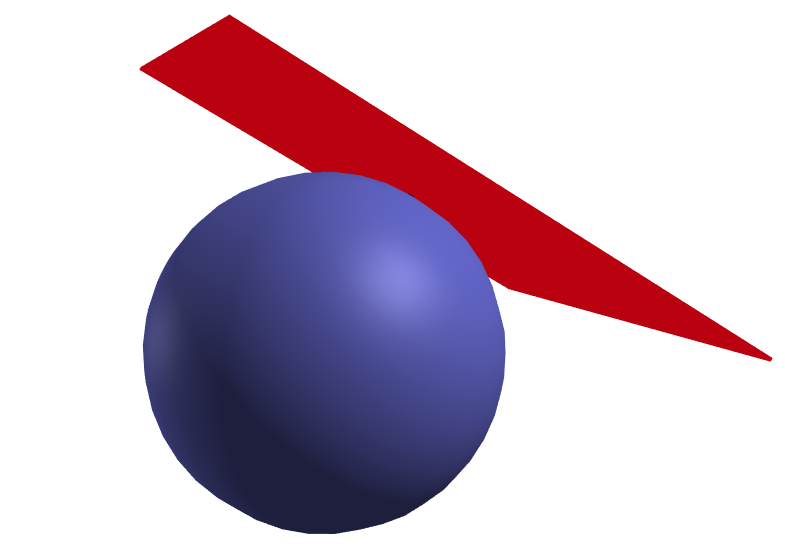
\includegraphics[height=5cm]{figures/tangent_plane.tikz}
        \caption{
            When linearizing about a point $q$ on an sphere $\mathbb{S}^{n-1}$ in 
            n-dimensional space, the tangent space $T$ is a plane living in $\R^{n-1}$, 
            illustrated here with $n=3$. Therefore, when linearizing about a unit 
            quaternion $q \in \Q$, the space of differential rotations lives in $\R^3$.
        }
        \label{fig:tangent_plane}
    \end{figure}
        
        Derivatives consider the effect an infinitesimal perturbation to the input has on
        an infinitesimal perturbation to the output. For vector spaces, the composition
        of the perturbation with the nominal value is simple addition and the
        infinitesimal perturbation lives in the same space as the original vector. For
        unit quaternions, however, neither of these are true; instead, they compose
        according to \eqref{eq:quat_mult}, and infinitesimal unit quaternions are (to
        first order) confined to a 3-dimensional plane tangent to $\Q$ (see Fig.
        \ref{fig:tangent_plane}).

        The fact that differential unit quaternions are three-dimensional should make
        intuitive sense: Rotations are inherently three-dimensional and differential
        rotations should live in the same space as angular velocity, i.e. $\R^3$.
        
        There are many possible three-parameter representations for small rotations in
        the literature. Many authors use the exponential map \cite{Baillieul1978,
        Zefran1998, Lee2008, Saccon2013, Sola2017, Fan2016, watterson2018trajectory},
        while others have used the Cayley map (also known as Rodrigues parameters)
        \cite{Kobilarov2011, Kobilarov2014}, Modified Rodrigues Parameters (MRPs)
        \cite{Terzakis2018}, or the vector part of the quaternion \cite{Fresk2013}.
        We choose Rodrigues parameters \cite{markley2014fundamentals} because they are
        computationally efficient and do not inherit the sign ambiguity associated with
        unit quaternions. The mapping between a vector of Rodrigues parameters $\phi \in
        \R^3$ and a unit quaternion $q$ is known as the Cayley map: \begin{equation}
        \label{eq:cayley}
            q = \varphi(\phi) = \frac{1}{\sqrt{1 + \norm{\phi}^2}} \begin{bmatrix} 1 \\ \phi \end{bmatrix}.
        \end{equation}
        We will also make use of the inverse Cayley map:
        \begin{equation}
            \phi = \varphi^{-1}(q) = \frac{q_v}{q_s}.
        \end{equation}

    \subsection{Jacobian of Vector-Valued Functions}
        When taking derivatives with respect to quaternions, we must take into account
        both the composition rule and the nonlinear mapping between the space of unit
        quaternions and our chosen three-parameter error representation.

        Let $\phi \in \R^3$ be a differential rotation applied to a function with
        quaternion inputs $y = h(q): \Q \to \R^p$, such that
        \begin{equation} \label{eq:vector_function}
            y + \delta y = h(L(q) \varphi(\phi)) \approx h(q) +  \nabla h(q) \phi.
        \end{equation}
        We can calculate the Jacobian $\nabla h(q) \in \R^{p \times 3}$ by
        differentiating \eqref{eq:vector_function} with respect to $\phi$, evaluated at
        $\phi = 0$:
        \begin{equation} \label{eq:quat_gradient}
            \nabla h(q) = \pdv{h}{q} L(q) H := \pdv{h}{q} G(q) 
                        = \pdv{h}{q} \begin{bmatrix} 
                            -q_v^T \\ 
                            sI_3 + \skewmat{q_v}
                        \end{bmatrix}
        \end{equation}
        where $G(q) \in \R^{4 \times 3}$ is the \textit{attitude Jacobian}, which
        essentially becomes a ``conversion factor'' allowing us to apply results from
        standard vector calculus to the space of unit quaternions. This form is
        particularly useful in practice since $\pdv*{h}{q} \in \R^{p \times 4}$ can be
        obtained using finite difference or automatic differentiation.
        As an aside, although we have used Rodrigues parameters, $G(q)$ is actually the
        same (up to a constant scaling factor) for any choice of three-parameter attitude
        representation.

    \subsection{Hessian of Scalar-Valued Functions}
	    If the output of $h$ is a scalar ($p = 1$), then we can find its Hessian by
	    taking the Jacobian of \eqref{eq:quat_gradient} with respect to $\phi$ using the
        product rule, again evaluated at $\phi = 0$:

	    \begin{equation} \label{eq:quat_hessian}
            \nabla^2 h(q) = G(q)^T \pdv[2]{h}{q} G(q) + I_3 \pdv{h}{q}q,
	    \end{equation}
	    where the second term comes from the second derivative of $\varphi(\phi)$.
	    Similar to $G(q)$, this ends up being the same (up to a scaling factor) for any
        choice of three-parameter attitude representation.
        
    \subsection{Jacobian of Quaternion-Valued Functions}
        We now consider the case of a function that maps unit quaternions to unit
        quaternions, $q' = f(q) : \Q \to \Q$. Here we must also consider the non-trivial
        effect of a differential value applied to the output, i.e.:
        \begin{equation} \label{eq:dqoutput}
            L(q') \varphi(\phi') = f(L(q)\varphi(\phi)) .
        \end{equation}
        Solving \eqref{eq:dqoutput} for $\phi'$ we find,
        \begin{equation} \label{eq:phiprime}
            \phi' = \varphi^{-1} \left( L(q')^T f(L(q)\varphi(\phi)) \right) \approx \nabla f(q) \, \phi.
        \end{equation}
        Finally, the desired Jacobian is obtained by taking the derivative of
        \eqref{eq:phiprime} with respect to $\phi$:
        \begin{equation} \label{eq:quat_jacobian}
            \nabla f(q) = H^T L(q')^T \pdv{f}{q} L(q) H = G(q')^T \pdv{f}{q} G(q).
        \end{equation}
        The leading $G(q')^T$ comes from the fact that as $\phi' \to 0$, $L(q') f(q) \to
        I_q$, where $I_q$ is the quaternion identity. Differentiating through the inverse
        map, evaluated at the quaternion identity, we find that $\pdv*{\varphi^{-1}}{q}
        \to H^T$ for any three-parameter attitude representation.


\section{Modifying Newton's Method} \label{sec:Wahbas}
    Newton's method uses derivative information about a function to iteratively approximate it's roots. For unconstrained systems, this method is highly effective, and can exhibit quadratic convergence.  For constrained systems, the updated parameter can be projected back onto the feasible set at each iteration, but without the same convergence guarantees. For the constraints on $SO(3)$, Newton's method struggles to converge past a certain threshold due to this projection. By leveraging the quaternion calculus introduced, Newton's method can be modified to implicitly account for these constraints. To demonstrate this, we will examine Wahba's Problem. In 1965, Grace Wahba proposed the criterion for a least squares estimate of a spacecraft's attitude from vector measurements \cite{markley2014fundamentals}. We will solve this problem using a standard nonlinear least squares method, as well as a method that exploits the true group structure of $SO(3)$ using the quaternion calculus presented here. 
    

    \subsection{Methodology}
    
    Given known vectors in some inertial frame, $N$, and measurements of these vectors in some body fixed frame, $B$, we can define Wahba's loss function as the following:
    \begin{equation}
        L = \sum_i w_i \| ^N v_i -  {}^N A(q){}^B\,\,  ^Bv_i \|_2^2.
    \end{equation}
    This is a nonlinear function of the attitude, which will be stored as a quaternion. For convenience, the following residual vector function will be defined:
    \begin{equation}
        r_i = \sqrt{w_i} (^N v_i -  {}^N A(q){}^B\,\,  ^Bv_i ),
    \end{equation}
    such that when these vectors are stacked in $r$, the loss function is a sum of squares. This problem now looks like a standard nonlinear least squares problem:
    \begin{mini*}
    {q}{ \|r(q)\|_2^2 }{}{}
    \addConstraint { q\in SO(3).}
    \end{mini*}
     There are two methods for keeping the solution in the $SO(3)$, group, a projected and a multiplicative method. In a projected Gauss-Newton method, the Newton step is applied additively, and the resulting estimate is projected back onto $SO(3)$ with a normalization. This algorithm can be seen in algorithm \ref{alg:pgn}. 
    \begin{algorithm} 
    	\begin{algorithmic}[1]
    		\caption{Projected Gauss-Newton Method}\label{alg:pgn}
    		\State $k = 0$
    		\While{significant progress}
    		    \State $J = \frac{\partial r(q_k)}{ \partial q}$ 
    		    \State $ q_{step} = -(J^TJ)^{-1}J^T r(q_k)$ 
    		  %  \State $q_{n+1} = \text{normalize}(q_n + q_{step})$ 
    		  \State $q_{k+1} = \Pi_{SO(3)}(q_k + q_{step})$ 
    		    \State $k = k + 1$
    		\EndWhile
    	\end{algorithmic}
    \end{algorithm}
    Where the $SO(3)$ projection operator is just a normalization. This method can successfully lower the loss function initially, but the normalization errors will prevent convergence. To get around this, the quaternion calculus presented in this paper can be used to generate a Newton step that is a three parameter rotation, one that can be applied multiplicatively. This method of applying the Newton step preserves the constraint satisfaction, and doesn't introduce any normalization errors.
    \begin{algorithm} 
    	\begin{algorithmic}[1]
    		\caption{Multiplicative Gauss-Newton Method}\label{alg:mgn}
    		\State $k = 0$
    		\While{significant progress}
    		    \State $J = [\frac{\partial r(q_k)}{ \partial q}]G(q_k)$ \Comment{quaternion adjusted Jacobian}
    		    \State $ \phi_{step} = -(J^TJ)^{-1}J^T r(q_k)$ 
    		    \State $q_{step} = \varphi(\phi_{step})$ 
    		    \State $q_{k+1} = q_n \otimes q_{step}$ \Comment{apply step multiplicatively}
    		    \State $k = k + 1$
    		\EndWhile
    	\end{algorithmic}
    \end{algorithm}


    \subsection{Results}
    % \begin{figure}
    %     \centering
    %     % This file was created by matlab2tikz.
%
%The latest updates can be retrieved from
%  http://www.mathworks.com/matlabcentral/fileexchange/22022-matlab2tikz-matlab2tikz
%where you can also make suggestions and rate matlab2tikz.
%
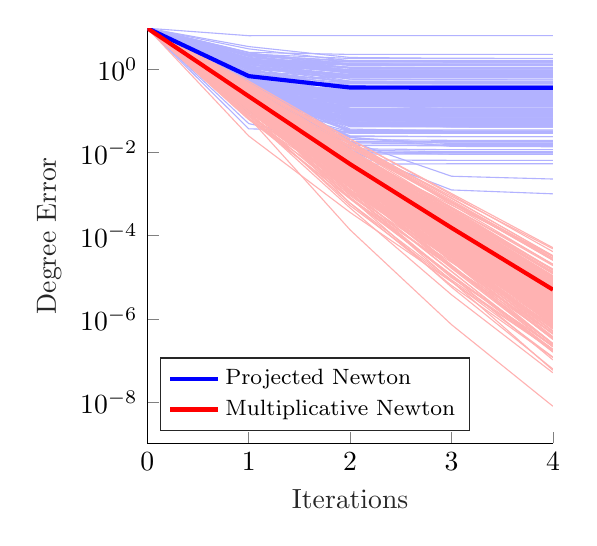
\begin{tikzpicture}

\begin{axis}[%
width=2.028in,
height=2.0754in,
at={(1.011in,0.642in)},
scale only axis,
unbounded coords=jump,
xmin=0,
xmax=4,
xlabel style={font=\color{white!15!black}},
xlabel={Iterations},
ymode=log,
ymin=1e-09,
ymax=10,
yminorticks=true,
ylabel style={font=\color{white!15!black}},
ylabel={Degree Error},
axis background/.style={fill=white},
title style={font=\bfseries},
% title={Solving Wahba's Problem with Newton's Method},
axis x line*=bottom,
axis y line*=left,
legend style={at={(0.03,0.03)}, anchor=south west, legend cell align=left, align=left, draw=white!15!black}
]
\addplot [color=white!70!blue, forget plot]
  table[row sep=crcr]{%
0	10\\
1	0.245349331902658\\
2	0.0333633371901889\\
3	0.0325688480496246\\
4	0.0325688480495408\\
5	nan\\
6	nan\\
7	nan\\
8	nan\\
9	nan\\
10	nan\\
11	nan\\
12	nan\\
13	nan\\
14	nan\\
15	nan\\
16	nan\\
17	nan\\
18	nan\\
19	nan\\
20	nan\\
};
\addplot [color=white!70!blue, forget plot]
  table[row sep=crcr]{%
0	10\\
1	0.256693089501186\\
2	0.116094795964189\\
3	0.114029965615891\\
4	0.113967665527987\\
5	nan\\
6	nan\\
7	nan\\
8	nan\\
9	nan\\
10	nan\\
11	nan\\
12	nan\\
13	nan\\
14	nan\\
15	nan\\
16	nan\\
17	nan\\
18	nan\\
19	nan\\
20	nan\\
};
\addplot [color=white!70!blue, forget plot]
  table[row sep=crcr]{%
0	10\\
1	0.501034993202954\\
2	0.144966088509281\\
3	0.144966088509281\\
4	0.144966088509281\\
5	nan\\
6	nan\\
7	nan\\
8	nan\\
9	nan\\
10	nan\\
11	nan\\
12	nan\\
13	nan\\
14	nan\\
15	nan\\
16	nan\\
17	nan\\
18	nan\\
19	nan\\
20	nan\\
};
\addplot [color=white!70!blue, forget plot]
  table[row sep=crcr]{%
0	10\\
1	1.2736554190532\\
2	0.097827905010807\\
3	0.0550766988621844\\
4	0.0531825745110992\\
5	nan\\
6	nan\\
7	nan\\
8	nan\\
9	nan\\
10	nan\\
11	nan\\
12	nan\\
13	nan\\
14	nan\\
15	nan\\
16	nan\\
17	nan\\
18	nan\\
19	nan\\
20	nan\\
};
\addplot [color=white!70!blue, forget plot]
  table[row sep=crcr]{%
0	10\\
1	1.55096899187761\\
2	0.991075271068435\\
3	0.990490526100744\\
4	0.990059336565758\\
5	nan\\
6	nan\\
7	nan\\
8	nan\\
9	nan\\
10	nan\\
11	nan\\
12	nan\\
13	nan\\
14	nan\\
15	nan\\
16	nan\\
17	nan\\
18	nan\\
19	nan\\
20	nan\\
};
\addplot [color=white!70!blue, forget plot]
  table[row sep=crcr]{%
0	10\\
1	0.321662295275667\\
2	0.198912905067804\\
3	0.197523008152883\\
4	0.197508865254868\\
5	nan\\
6	nan\\
7	nan\\
8	nan\\
9	nan\\
10	nan\\
11	nan\\
12	nan\\
13	nan\\
14	nan\\
15	nan\\
16	nan\\
17	nan\\
18	nan\\
19	nan\\
20	nan\\
};
\addplot [color=white!70!blue, forget plot]
  table[row sep=crcr]{%
0	10\\
1	0.489141458693822\\
2	0.0104334557249363\\
3	0.0102529071563397\\
4	0.0102529071014911\\
5	nan\\
6	nan\\
7	nan\\
8	nan\\
9	nan\\
10	nan\\
11	nan\\
12	nan\\
13	nan\\
14	nan\\
15	nan\\
16	nan\\
17	nan\\
18	nan\\
19	nan\\
20	nan\\
};
\addplot [color=white!70!blue, forget plot]
  table[row sep=crcr]{%
0	10\\
1	0.295763804059839\\
2	0.0651487706647099\\
3	0.0651487706649578\\
4	0.0651487706649578\\
5	nan\\
6	nan\\
7	nan\\
8	nan\\
9	nan\\
10	nan\\
11	nan\\
12	nan\\
13	nan\\
14	nan\\
15	nan\\
16	nan\\
17	nan\\
18	nan\\
19	nan\\
20	nan\\
};
\addplot [color=white!70!blue, forget plot]
  table[row sep=crcr]{%
0	9.99999999999999\\
1	3.18267528830554\\
2	1.64339591697523\\
3	1.53163679238799\\
4	1.52760015839945\\
5	nan\\
6	nan\\
7	nan\\
8	nan\\
9	nan\\
10	nan\\
11	nan\\
12	nan\\
13	nan\\
14	nan\\
15	nan\\
16	nan\\
17	nan\\
18	nan\\
19	nan\\
20	nan\\
};
\addplot [color=white!70!blue, forget plot]
  table[row sep=crcr]{%
0	10\\
1	1.70078531141711\\
2	1.14670244235688\\
3	1.13952405721556\\
4	1.13924468140824\\
5	nan\\
6	nan\\
7	nan\\
8	nan\\
9	nan\\
10	nan\\
11	nan\\
12	nan\\
13	nan\\
14	nan\\
15	nan\\
16	nan\\
17	nan\\
18	nan\\
19	nan\\
20	nan\\
};
\addplot [color=white!70!blue, forget plot]
  table[row sep=crcr]{%
0	9.99999999999999\\
1	1.05848945742852\\
2	0.30652503011972\\
3	0.301066066437304\\
4	0.300976995295993\\
5	nan\\
6	nan\\
7	nan\\
8	nan\\
9	nan\\
10	nan\\
11	nan\\
12	nan\\
13	nan\\
14	nan\\
15	nan\\
16	nan\\
17	nan\\
18	nan\\
19	nan\\
20	nan\\
};
\addplot [color=white!70!blue, forget plot]
  table[row sep=crcr]{%
0	9.99999999999999\\
1	3.61419288482415\\
2	1.97236599479523\\
3	1.88670262073814\\
4	1.88445234597056\\
5	nan\\
6	nan\\
7	nan\\
8	nan\\
9	nan\\
10	nan\\
11	nan\\
12	nan\\
13	nan\\
14	nan\\
15	nan\\
16	nan\\
17	nan\\
18	nan\\
19	nan\\
20	nan\\
};
\addplot [color=white!70!blue, forget plot]
  table[row sep=crcr]{%
0	10\\
1	0.256935248082493\\
2	0.0657146651782446\\
3	0.0663935882691914\\
4	0.0663935882696225\\
5	nan\\
6	nan\\
7	nan\\
8	nan\\
9	nan\\
10	nan\\
11	nan\\
12	nan\\
13	nan\\
14	nan\\
15	nan\\
16	nan\\
17	nan\\
18	nan\\
19	nan\\
20	nan\\
};
\addplot [color=white!70!blue, forget plot]
  table[row sep=crcr]{%
0	10\\
1	0.469824863188568\\
2	0.172164547023073\\
3	0.170973291574881\\
4	0.170951880184027\\
5	nan\\
6	nan\\
7	nan\\
8	nan\\
9	nan\\
10	nan\\
11	nan\\
12	nan\\
13	nan\\
14	nan\\
15	nan\\
16	nan\\
17	nan\\
18	nan\\
19	nan\\
20	nan\\
};
\addplot [color=white!70!blue, forget plot]
  table[row sep=crcr]{%
0	9.99999999999999\\
1	1.32785592600248\\
2	0.871588490840145\\
3	0.864115233201693\\
4	0.863867395536786\\
5	nan\\
6	nan\\
7	nan\\
8	nan\\
9	nan\\
10	nan\\
11	nan\\
12	nan\\
13	nan\\
14	nan\\
15	nan\\
16	nan\\
17	nan\\
18	nan\\
19	nan\\
20	nan\\
};
\addplot [color=white!70!blue, forget plot]
  table[row sep=crcr]{%
0	10\\
1	0.286194765961565\\
2	0.0180521175540148\\
3	0.0180222488608033\\
4	0.0180222488612391\\
5	nan\\
6	nan\\
7	nan\\
8	nan\\
9	nan\\
10	nan\\
11	nan\\
12	nan\\
13	nan\\
14	nan\\
15	nan\\
16	nan\\
17	nan\\
18	nan\\
19	nan\\
20	nan\\
};
\addplot [color=white!70!blue, forget plot]
  table[row sep=crcr]{%
0	10\\
1	1.69845382772434\\
2	1.58690411478842\\
3	1.58690411478842\\
4	1.58690411478842\\
5	nan\\
6	nan\\
7	nan\\
8	nan\\
9	nan\\
10	nan\\
11	nan\\
12	nan\\
13	nan\\
14	nan\\
15	nan\\
16	nan\\
17	nan\\
18	nan\\
19	nan\\
20	nan\\
};
\addplot [color=white!70!blue, forget plot]
  table[row sep=crcr]{%
0	10\\
1	0.346289884668588\\
2	0.0235549532597901\\
3	0.0142266638285708\\
4	0.0139624019738922\\
5	nan\\
6	nan\\
7	nan\\
8	nan\\
9	nan\\
10	nan\\
11	nan\\
12	nan\\
13	nan\\
14	nan\\
15	nan\\
16	nan\\
17	nan\\
18	nan\\
19	nan\\
20	nan\\
};
\addplot [color=white!70!blue, forget plot]
  table[row sep=crcr]{%
0	10\\
1	0.401340950064376\\
2	0.27566221584103\\
3	0.27566221584103\\
4	0.27566221584103\\
5	nan\\
6	nan\\
7	nan\\
8	nan\\
9	nan\\
10	nan\\
11	nan\\
12	nan\\
13	nan\\
14	nan\\
15	nan\\
16	nan\\
17	nan\\
18	nan\\
19	nan\\
20	nan\\
};
\addplot [color=white!70!blue, forget plot]
  table[row sep=crcr]{%
0	10\\
1	1.57871793724352\\
2	1.10016400760137\\
3	1.08482415905096\\
4	1.08426743295854\\
5	nan\\
6	nan\\
7	nan\\
8	nan\\
9	nan\\
10	nan\\
11	nan\\
12	nan\\
13	nan\\
14	nan\\
15	nan\\
16	nan\\
17	nan\\
18	nan\\
19	nan\\
20	nan\\
};
\addplot [color=white!70!blue, forget plot]
  table[row sep=crcr]{%
0	9.99999999999999\\
1	0.383913093336153\\
2	0.356839781269237\\
3	0.356839781269299\\
4	0.356839781269305\\
5	nan\\
6	nan\\
7	nan\\
8	nan\\
9	nan\\
10	nan\\
11	nan\\
12	nan\\
13	nan\\
14	nan\\
15	nan\\
16	nan\\
17	nan\\
18	nan\\
19	nan\\
20	nan\\
};
\addplot [color=white!70!blue, forget plot]
  table[row sep=crcr]{%
0	10\\
1	0.682009818252721\\
2	0.362191598154435\\
3	0.362323009276128\\
4	0.362323009276128\\
5	nan\\
6	nan\\
7	nan\\
8	nan\\
9	nan\\
10	nan\\
11	nan\\
12	nan\\
13	nan\\
14	nan\\
15	nan\\
16	nan\\
17	nan\\
18	nan\\
19	nan\\
20	nan\\
};
\addplot [color=white!70!blue, forget plot]
  table[row sep=crcr]{%
0	9.99999999999999\\
1	0.151416599377896\\
2	0.0316437952149763\\
3	0.0313764886459332\\
4	0.0313739379426789\\
5	nan\\
6	nan\\
7	nan\\
8	nan\\
9	nan\\
10	nan\\
11	nan\\
12	nan\\
13	nan\\
14	nan\\
15	nan\\
16	nan\\
17	nan\\
18	nan\\
19	nan\\
20	nan\\
};
\addplot [color=white!70!blue, forget plot]
  table[row sep=crcr]{%
0	10\\
1	0.59764676144237\\
2	0.382130656403886\\
3	0.379770313780982\\
4	0.379760444777267\\
5	nan\\
6	nan\\
7	nan\\
8	nan\\
9	nan\\
10	nan\\
11	nan\\
12	nan\\
13	nan\\
14	nan\\
15	nan\\
16	nan\\
17	nan\\
18	nan\\
19	nan\\
20	nan\\
};
\addplot [color=white!70!blue, forget plot]
  table[row sep=crcr]{%
0	9.99999999999999\\
1	0.329127697782025\\
2	0.0230958929308416\\
3	0.0166077667654762\\
4	0.0164565913687051\\
5	nan\\
6	nan\\
7	nan\\
8	nan\\
9	nan\\
10	nan\\
11	nan\\
12	nan\\
13	nan\\
14	nan\\
15	nan\\
16	nan\\
17	nan\\
18	nan\\
19	nan\\
20	nan\\
};
\addplot [color=white!70!blue, forget plot]
  table[row sep=crcr]{%
0	10\\
1	0.150768591238384\\
2	0.0889548935647755\\
3	0.0889548935647774\\
4	0.0889548935647774\\
5	nan\\
6	nan\\
7	nan\\
8	nan\\
9	nan\\
10	nan\\
11	nan\\
12	nan\\
13	nan\\
14	nan\\
15	nan\\
16	nan\\
17	nan\\
18	nan\\
19	nan\\
20	nan\\
};
\addplot [color=white!70!blue, forget plot]
  table[row sep=crcr]{%
0	10\\
1	0.355315151334663\\
2	0.256224232049653\\
3	0.256224232049653\\
4	0.256224232049653\\
5	nan\\
6	nan\\
7	nan\\
8	nan\\
9	nan\\
10	nan\\
11	nan\\
12	nan\\
13	nan\\
14	nan\\
15	nan\\
16	nan\\
17	nan\\
18	nan\\
19	nan\\
20	nan\\
};
\addplot [color=white!70!blue, forget plot]
  table[row sep=crcr]{%
0	9.99999999999999\\
1	0.915158689475732\\
2	0.648483498989128\\
3	0.64848349898913\\
4	0.648483498989134\\
5	nan\\
6	nan\\
7	nan\\
8	nan\\
9	nan\\
10	nan\\
11	nan\\
12	nan\\
13	nan\\
14	nan\\
15	nan\\
16	nan\\
17	nan\\
18	nan\\
19	nan\\
20	nan\\
};
\addplot [color=white!70!blue, forget plot]
  table[row sep=crcr]{%
0	9.99999999999999\\
1	0.497964939692414\\
2	0.221687111679754\\
3	0.221109764103814\\
4	0.221109764103814\\
5	nan\\
6	nan\\
7	nan\\
8	nan\\
9	nan\\
10	nan\\
11	nan\\
12	nan\\
13	nan\\
14	nan\\
15	nan\\
16	nan\\
17	nan\\
18	nan\\
19	nan\\
20	nan\\
};
\addplot [color=white!70!blue, forget plot]
  table[row sep=crcr]{%
0	10\\
1	0.290387838607823\\
2	0.062371892734605\\
3	0.062371892734605\\
4	0.062371892734605\\
5	nan\\
6	nan\\
7	nan\\
8	nan\\
9	nan\\
10	nan\\
11	nan\\
12	nan\\
13	nan\\
14	nan\\
15	nan\\
16	nan\\
17	nan\\
18	nan\\
19	nan\\
20	nan\\
};
\addplot [color=white!70!blue, forget plot]
  table[row sep=crcr]{%
0	9.99999999999999\\
1	0.28697575159076\\
2	0.0104433587968458\\
3	0.00920133333420638\\
4	0.00920133333421795\\
5	nan\\
6	nan\\
7	nan\\
8	nan\\
9	nan\\
10	nan\\
11	nan\\
12	nan\\
13	nan\\
14	nan\\
15	nan\\
16	nan\\
17	nan\\
18	nan\\
19	nan\\
20	nan\\
};
\addplot [color=white!70!blue, forget plot]
  table[row sep=crcr]{%
0	10\\
1	1.60872376052541\\
2	0.81562182024763\\
3	0.801292941126267\\
4	0.801175412053152\\
5	nan\\
6	nan\\
7	nan\\
8	nan\\
9	nan\\
10	nan\\
11	nan\\
12	nan\\
13	nan\\
14	nan\\
15	nan\\
16	nan\\
17	nan\\
18	nan\\
19	nan\\
20	nan\\
};
\addplot [color=white!70!blue, forget plot]
  table[row sep=crcr]{%
0	9.99999999999999\\
1	0.432375728078319\\
2	0.0853463702929169\\
3	0.0833034562697832\\
4	0.0832399513020398\\
5	nan\\
6	nan\\
7	nan\\
8	nan\\
9	nan\\
10	nan\\
11	nan\\
12	nan\\
13	nan\\
14	nan\\
15	nan\\
16	nan\\
17	nan\\
18	nan\\
19	nan\\
20	nan\\
};
\addplot [color=white!70!blue, forget plot]
  table[row sep=crcr]{%
0	10\\
1	0.303360256704549\\
2	0.243704430205994\\
3	0.24253334245811\\
4	0.242533342458155\\
5	nan\\
6	nan\\
7	nan\\
8	nan\\
9	nan\\
10	nan\\
11	nan\\
12	nan\\
13	nan\\
14	nan\\
15	nan\\
16	nan\\
17	nan\\
18	nan\\
19	nan\\
20	nan\\
};
\addplot [color=white!70!blue, forget plot]
  table[row sep=crcr]{%
0	9.99999999999999\\
1	0.214311633037256\\
2	0.0630947679712425\\
3	0.0618091878911565\\
4	0.0617816568512434\\
5	nan\\
6	nan\\
7	nan\\
8	nan\\
9	nan\\
10	nan\\
11	nan\\
12	nan\\
13	nan\\
14	nan\\
15	nan\\
16	nan\\
17	nan\\
18	nan\\
19	nan\\
20	nan\\
};
\addplot [color=white!70!blue, forget plot]
  table[row sep=crcr]{%
0	10\\
1	0.342837912247771\\
2	0.342837912247781\\
3	0.342837912247791\\
4	0.342837912247813\\
5	nan\\
6	nan\\
7	nan\\
8	nan\\
9	nan\\
10	nan\\
11	nan\\
12	nan\\
13	nan\\
14	nan\\
15	nan\\
16	nan\\
17	nan\\
18	nan\\
19	nan\\
20	nan\\
};
\addplot [color=white!70!blue, forget plot]
  table[row sep=crcr]{%
0	10\\
1	0.0503280676541876\\
2	0.015195942036944\\
3	0.015195942036944\\
4	0.015195942036944\\
5	nan\\
6	nan\\
7	nan\\
8	nan\\
9	nan\\
10	nan\\
11	nan\\
12	nan\\
13	nan\\
14	nan\\
15	nan\\
16	nan\\
17	nan\\
18	nan\\
19	nan\\
20	nan\\
};
\addplot [color=white!70!blue, forget plot]
  table[row sep=crcr]{%
0	10\\
1	0.340090081997174\\
2	0.199101320878426\\
3	0.198563231091935\\
4	0.198563231091946\\
5	nan\\
6	nan\\
7	nan\\
8	nan\\
9	nan\\
10	nan\\
11	nan\\
12	nan\\
13	nan\\
14	nan\\
15	nan\\
16	nan\\
17	nan\\
18	nan\\
19	nan\\
20	nan\\
};
\addplot [color=white!70!blue, forget plot]
  table[row sep=crcr]{%
0	9.99999999999999\\
1	0.413428328243305\\
2	0.0746489203279725\\
3	0.0678034655760613\\
4	0.0676019920980228\\
5	nan\\
6	nan\\
7	nan\\
8	nan\\
9	nan\\
10	nan\\
11	nan\\
12	nan\\
13	nan\\
14	nan\\
15	nan\\
16	nan\\
17	nan\\
18	nan\\
19	nan\\
20	nan\\
};
\addplot [color=white!70!blue, forget plot]
  table[row sep=crcr]{%
0	10\\
1	1.464527920238\\
2	1.46452792023801\\
3	1.46452792023801\\
4	1.46452792023801\\
5	nan\\
6	nan\\
7	nan\\
8	nan\\
9	nan\\
10	nan\\
11	nan\\
12	nan\\
13	nan\\
14	nan\\
15	nan\\
16	nan\\
17	nan\\
18	nan\\
19	nan\\
20	nan\\
};
\addplot [color=white!70!blue, forget plot]
  table[row sep=crcr]{%
0	10\\
1	0.179253915156114\\
2	0.0604214678016003\\
3	0.0604214678016003\\
4	0.0604214678016003\\
5	nan\\
6	nan\\
7	nan\\
8	nan\\
9	nan\\
10	nan\\
11	nan\\
12	nan\\
13	nan\\
14	nan\\
15	nan\\
16	nan\\
17	nan\\
18	nan\\
19	nan\\
20	nan\\
};
\addplot [color=white!70!blue, forget plot]
  table[row sep=crcr]{%
0	9.99999999999999\\
1	2.62565087582375\\
2	2.33789675976232\\
3	2.33789675976232\\
4	2.33789675976232\\
5	nan\\
6	nan\\
7	nan\\
8	nan\\
9	nan\\
10	nan\\
11	nan\\
12	nan\\
13	nan\\
14	nan\\
15	nan\\
16	nan\\
17	nan\\
18	nan\\
19	nan\\
20	nan\\
};
\addplot [color=white!70!blue, forget plot]
  table[row sep=crcr]{%
0	10\\
1	0.328830674317276\\
2	0.329874079047322\\
3	0.329874079047322\\
4	0.329874079047322\\
5	nan\\
6	nan\\
7	nan\\
8	nan\\
9	nan\\
10	nan\\
11	nan\\
12	nan\\
13	nan\\
14	nan\\
15	nan\\
16	nan\\
17	nan\\
18	nan\\
19	nan\\
20	nan\\
};
\addplot [color=white!70!blue, forget plot]
  table[row sep=crcr]{%
0	10\\
1	0.461281190697483\\
2	0.461281190697489\\
3	0.461281190697489\\
4	0.461281190697489\\
5	nan\\
6	nan\\
7	nan\\
8	nan\\
9	nan\\
10	nan\\
11	nan\\
12	nan\\
13	nan\\
14	nan\\
15	nan\\
16	nan\\
17	nan\\
18	nan\\
19	nan\\
20	nan\\
};
\addplot [color=white!70!blue, forget plot]
  table[row sep=crcr]{%
0	9.99999999999999\\
1	0.302536003661621\\
2	0.0185535785137764\\
3	0.0185535785138451\\
4	0.0185535785139132\\
5	nan\\
6	nan\\
7	nan\\
8	nan\\
9	nan\\
10	nan\\
11	nan\\
12	nan\\
13	nan\\
14	nan\\
15	nan\\
16	nan\\
17	nan\\
18	nan\\
19	nan\\
20	nan\\
};
\addplot [color=white!70!blue, forget plot]
  table[row sep=crcr]{%
0	10\\
1	0.212106814608706\\
2	0.0604846655963059\\
3	0.0587110592824785\\
4	0.0586708860451671\\
5	nan\\
6	nan\\
7	nan\\
8	nan\\
9	nan\\
10	nan\\
11	nan\\
12	nan\\
13	nan\\
14	nan\\
15	nan\\
16	nan\\
17	nan\\
18	nan\\
19	nan\\
20	nan\\
};
\addplot [color=white!70!blue, forget plot]
  table[row sep=crcr]{%
0	10\\
1	0.49098012952775\\
2	0.156530517281051\\
3	0.154708896844361\\
4	0.154672198121554\\
5	nan\\
6	nan\\
7	nan\\
8	nan\\
9	nan\\
10	nan\\
11	nan\\
12	nan\\
13	nan\\
14	nan\\
15	nan\\
16	nan\\
17	nan\\
18	nan\\
19	nan\\
20	nan\\
};
\addplot [color=white!70!blue, forget plot]
  table[row sep=crcr]{%
0	9.99999999999999\\
1	0.593326892523197\\
2	0.0524264491516143\\
3	0.0419392897571128\\
4	0.0414436424610525\\
5	nan\\
6	nan\\
7	nan\\
8	nan\\
9	nan\\
10	nan\\
11	nan\\
12	nan\\
13	nan\\
14	nan\\
15	nan\\
16	nan\\
17	nan\\
18	nan\\
19	nan\\
20	nan\\
};
\addplot [color=white!70!blue, forget plot]
  table[row sep=crcr]{%
0	10\\
1	0.24370221808798\\
2	0.0244159301525864\\
3	0.0244159301531297\\
4	0.0244159301531372\\
5	nan\\
6	nan\\
7	nan\\
8	nan\\
9	nan\\
10	nan\\
11	nan\\
12	nan\\
13	nan\\
14	nan\\
15	nan\\
16	nan\\
17	nan\\
18	nan\\
19	nan\\
20	nan\\
};
\addplot [color=white!70!blue, forget plot]
  table[row sep=crcr]{%
0	10\\
1	0.78624562245936\\
2	0.352033877039429\\
3	0.349806152257134\\
4	0.349746167777541\\
5	nan\\
6	nan\\
7	nan\\
8	nan\\
9	nan\\
10	nan\\
11	nan\\
12	nan\\
13	nan\\
14	nan\\
15	nan\\
16	nan\\
17	nan\\
18	nan\\
19	nan\\
20	nan\\
};
\addplot [color=white!70!blue, forget plot]
  table[row sep=crcr]{%
0	10\\
1	0.337420405288078\\
2	0.0617526490683332\\
3	0.0557964991086933\\
4	0.055584387050265\\
5	nan\\
6	nan\\
7	nan\\
8	nan\\
9	nan\\
10	nan\\
11	nan\\
12	nan\\
13	nan\\
14	nan\\
15	nan\\
16	nan\\
17	nan\\
18	nan\\
19	nan\\
20	nan\\
};
\addplot [color=white!70!blue, forget plot]
  table[row sep=crcr]{%
0	9.99999999999999\\
1	1.64176404486337\\
2	1.3669912421168\\
3	1.35790646475612\\
4	1.35790646475612\\
5	nan\\
6	nan\\
7	nan\\
8	nan\\
9	nan\\
10	nan\\
11	nan\\
12	nan\\
13	nan\\
14	nan\\
15	nan\\
16	nan\\
17	nan\\
18	nan\\
19	nan\\
20	nan\\
};
\addplot [color=white!70!blue, forget plot]
  table[row sep=crcr]{%
0	9.99999999999999\\
1	0.0377780283719721\\
2	0.0318404292489432\\
3	0.0318404292489529\\
4	0.0318404292489529\\
5	nan\\
6	nan\\
7	nan\\
8	nan\\
9	nan\\
10	nan\\
11	nan\\
12	nan\\
13	nan\\
14	nan\\
15	nan\\
16	nan\\
17	nan\\
18	nan\\
19	nan\\
20	nan\\
};
\addplot [color=white!70!blue, forget plot]
  table[row sep=crcr]{%
0	9.99999999999999\\
1	0.170080778750597\\
2	0.0724652859908885\\
3	0.0728393202828249\\
4	0.0728393202828777\\
5	nan\\
6	nan\\
7	nan\\
8	nan\\
9	nan\\
10	nan\\
11	nan\\
12	nan\\
13	nan\\
14	nan\\
15	nan\\
16	nan\\
17	nan\\
18	nan\\
19	nan\\
20	nan\\
};
\addplot [color=white!70!blue, forget plot]
  table[row sep=crcr]{%
0	10\\
1	1.87608384490381\\
2	0.981990082810094\\
3	0.967373527699061\\
4	0.967097101937814\\
5	nan\\
6	nan\\
7	nan\\
8	nan\\
9	nan\\
10	nan\\
11	nan\\
12	nan\\
13	nan\\
14	nan\\
15	nan\\
16	nan\\
17	nan\\
18	nan\\
19	nan\\
20	nan\\
};
\addplot [color=white!70!blue, forget plot]
  table[row sep=crcr]{%
0	10\\
1	0.287305203838467\\
2	0.112941539250752\\
3	0.110526890101806\\
4	0.110490458079942\\
5	nan\\
6	nan\\
7	nan\\
8	nan\\
9	nan\\
10	nan\\
11	nan\\
12	nan\\
13	nan\\
14	nan\\
15	nan\\
16	nan\\
17	nan\\
18	nan\\
19	nan\\
20	nan\\
};
\addplot [color=white!70!blue, forget plot]
  table[row sep=crcr]{%
0	10\\
1	0.317356812166891\\
2	0.0914942656083108\\
3	0.0914942656083108\\
4	0.0914942656083108\\
5	nan\\
6	nan\\
7	nan\\
8	nan\\
9	nan\\
10	nan\\
11	nan\\
12	nan\\
13	nan\\
14	nan\\
15	nan\\
16	nan\\
17	nan\\
18	nan\\
19	nan\\
20	nan\\
};
\addplot [color=white!70!blue, forget plot]
  table[row sep=crcr]{%
0	10\\
1	0.225900168285479\\
2	0.115846482253708\\
3	0.11584648225385\\
4	0.115846482253844\\
5	nan\\
6	nan\\
7	nan\\
8	nan\\
9	nan\\
10	nan\\
11	nan\\
12	nan\\
13	nan\\
14	nan\\
15	nan\\
16	nan\\
17	nan\\
18	nan\\
19	nan\\
20	nan\\
};
\addplot [color=white!70!blue, forget plot]
  table[row sep=crcr]{%
0	9.99999999999999\\
1	0.229941848021501\\
2	0.0818857262493336\\
3	0.0803733150914882\\
4	0.0803253277252016\\
5	nan\\
6	nan\\
7	nan\\
8	nan\\
9	nan\\
10	nan\\
11	nan\\
12	nan\\
13	nan\\
14	nan\\
15	nan\\
16	nan\\
17	nan\\
18	nan\\
19	nan\\
20	nan\\
};
\addplot [color=white!70!blue, forget plot]
  table[row sep=crcr]{%
0	10\\
1	0.562158782641134\\
2	0.200245380567929\\
3	0.200245380567929\\
4	0.200245380567929\\
5	nan\\
6	nan\\
7	nan\\
8	nan\\
9	nan\\
10	nan\\
11	nan\\
12	nan\\
13	nan\\
14	nan\\
15	nan\\
16	nan\\
17	nan\\
18	nan\\
19	nan\\
20	nan\\
};
\addplot [color=white!70!blue, forget plot]
  table[row sep=crcr]{%
0	10\\
1	0.432829989646104\\
2	0.186932941372157\\
3	0.178842203848733\\
4	0.178842203848747\\
5	nan\\
6	nan\\
7	nan\\
8	nan\\
9	nan\\
10	nan\\
11	nan\\
12	nan\\
13	nan\\
14	nan\\
15	nan\\
16	nan\\
17	nan\\
18	nan\\
19	nan\\
20	nan\\
};
\addplot [color=white!70!blue, forget plot]
  table[row sep=crcr]{%
0	10\\
1	0.318489106332649\\
2	0.101885944625254\\
3	0.101885944625288\\
4	0.101885944625288\\
5	nan\\
6	nan\\
7	nan\\
8	nan\\
9	nan\\
10	nan\\
11	nan\\
12	nan\\
13	nan\\
14	nan\\
15	nan\\
16	nan\\
17	nan\\
18	nan\\
19	nan\\
20	nan\\
};
\addplot [color=white!70!blue, forget plot]
  table[row sep=crcr]{%
0	10\\
1	0.838454660049197\\
2	0.0188052870160106\\
3	0.00271590068120344\\
4	0.00232901557533258\\
5	nan\\
6	nan\\
7	nan\\
8	nan\\
9	nan\\
10	nan\\
11	nan\\
12	nan\\
13	nan\\
14	nan\\
15	nan\\
16	nan\\
17	nan\\
18	nan\\
19	nan\\
20	nan\\
};
\addplot [color=white!70!blue, forget plot]
  table[row sep=crcr]{%
0	10\\
1	0.320557017932316\\
2	0.319077706447446\\
3	0.319077706447449\\
4	0.319077706447479\\
5	nan\\
6	nan\\
7	nan\\
8	nan\\
9	nan\\
10	nan\\
11	nan\\
12	nan\\
13	nan\\
14	nan\\
15	nan\\
16	nan\\
17	nan\\
18	nan\\
19	nan\\
20	nan\\
};
\addplot [color=white!70!blue, forget plot]
  table[row sep=crcr]{%
0	9.99999999999999\\
1	0.369926703046224\\
2	0.0316814625159715\\
3	0.0316814625160054\\
4	0.0316814625160054\\
5	nan\\
6	nan\\
7	nan\\
8	nan\\
9	nan\\
10	nan\\
11	nan\\
12	nan\\
13	nan\\
14	nan\\
15	nan\\
16	nan\\
17	nan\\
18	nan\\
19	nan\\
20	nan\\
};
\addplot [color=white!70!blue, forget plot]
  table[row sep=crcr]{%
0	10\\
1	0.270032528034605\\
2	0.0479771710045079\\
3	0.0479771710046175\\
4	0.0479771710046443\\
5	nan\\
6	nan\\
7	nan\\
8	nan\\
9	nan\\
10	nan\\
11	nan\\
12	nan\\
13	nan\\
14	nan\\
15	nan\\
16	nan\\
17	nan\\
18	nan\\
19	nan\\
20	nan\\
};
\addplot [color=white!70!blue, forget plot]
  table[row sep=crcr]{%
0	10\\
1	2.55196647852078\\
2	1.36904375348169\\
3	1.32831728065025\\
4	1.32711222494458\\
5	nan\\
6	nan\\
7	nan\\
8	nan\\
9	nan\\
10	nan\\
11	nan\\
12	nan\\
13	nan\\
14	nan\\
15	nan\\
16	nan\\
17	nan\\
18	nan\\
19	nan\\
20	nan\\
};
\addplot [color=white!70!blue, forget plot]
  table[row sep=crcr]{%
0	10\\
1	0.296797021963063\\
2	0.00528517480342902\\
3	0.00542487106371832\\
4	0.00542487106607597\\
5	nan\\
6	nan\\
7	nan\\
8	nan\\
9	nan\\
10	nan\\
11	nan\\
12	nan\\
13	nan\\
14	nan\\
15	nan\\
16	nan\\
17	nan\\
18	nan\\
19	nan\\
20	nan\\
};
\addplot [color=white!70!blue, forget plot]
  table[row sep=crcr]{%
0	10\\
1	0.0982531629902884\\
2	0.0460236521489956\\
3	0.0456956312650842\\
4	0.0456947083437279\\
5	nan\\
6	nan\\
7	nan\\
8	nan\\
9	nan\\
10	nan\\
11	nan\\
12	nan\\
13	nan\\
14	nan\\
15	nan\\
16	nan\\
17	nan\\
18	nan\\
19	nan\\
20	nan\\
};
\addplot [color=white!70!blue, forget plot]
  table[row sep=crcr]{%
0	10\\
1	0.451376725867608\\
2	0.208655059920608\\
3	0.208655059920608\\
4	0.208655059920608\\
5	nan\\
6	nan\\
7	nan\\
8	nan\\
9	nan\\
10	nan\\
11	nan\\
12	nan\\
13	nan\\
14	nan\\
15	nan\\
16	nan\\
17	nan\\
18	nan\\
19	nan\\
20	nan\\
};
\addplot [color=white!70!blue, forget plot]
  table[row sep=crcr]{%
0	10\\
1	0.821809577450768\\
2	0.531811905768021\\
3	0.52928116986549\\
4	0.529275263829724\\
5	nan\\
6	nan\\
7	nan\\
8	nan\\
9	nan\\
10	nan\\
11	nan\\
12	nan\\
13	nan\\
14	nan\\
15	nan\\
16	nan\\
17	nan\\
18	nan\\
19	nan\\
20	nan\\
};
\addplot [color=white!70!blue, forget plot]
  table[row sep=crcr]{%
0	10\\
1	0.518188705903385\\
2	0.0124449264164568\\
3	0.0118552561229174\\
4	0.0118552561230736\\
5	nan\\
6	nan\\
7	nan\\
8	nan\\
9	nan\\
10	nan\\
11	nan\\
12	nan\\
13	nan\\
14	nan\\
15	nan\\
16	nan\\
17	nan\\
18	nan\\
19	nan\\
20	nan\\
};
\addplot [color=white!70!blue, forget plot]
  table[row sep=crcr]{%
0	10\\
1	2.39473898459095\\
2	1.86732011445589\\
3	1.85641549453923\\
4	1.85621806769423\\
5	nan\\
6	nan\\
7	nan\\
8	nan\\
9	nan\\
10	nan\\
11	nan\\
12	nan\\
13	nan\\
14	nan\\
15	nan\\
16	nan\\
17	nan\\
18	nan\\
19	nan\\
20	nan\\
};
\addplot [color=white!70!blue, forget plot]
  table[row sep=crcr]{%
0	10\\
1	0.317783217997976\\
2	0.207703730260337\\
3	0.207043320240821\\
4	0.207027648909993\\
5	nan\\
6	nan\\
7	nan\\
8	nan\\
9	nan\\
10	nan\\
11	nan\\
12	nan\\
13	nan\\
14	nan\\
15	nan\\
16	nan\\
17	nan\\
18	nan\\
19	nan\\
20	nan\\
};
\addplot [color=white!70!blue, forget plot]
  table[row sep=crcr]{%
0	9.99999999999999\\
1	0.468967306931172\\
2	0.0338125883067714\\
3	0.0320088671455984\\
4	0.0319299124711627\\
5	nan\\
6	nan\\
7	nan\\
8	nan\\
9	nan\\
10	nan\\
11	nan\\
12	nan\\
13	nan\\
14	nan\\
15	nan\\
16	nan\\
17	nan\\
18	nan\\
19	nan\\
20	nan\\
};
\addplot [color=white!70!blue, forget plot]
  table[row sep=crcr]{%
0	10\\
1	0.55157946311789\\
2	0.381660400647596\\
3	0.381895428409426\\
4	0.381805810099611\\
5	nan\\
6	nan\\
7	nan\\
8	nan\\
9	nan\\
10	nan\\
11	nan\\
12	nan\\
13	nan\\
14	nan\\
15	nan\\
16	nan\\
17	nan\\
18	nan\\
19	nan\\
20	nan\\
};
\addplot [color=white!70!blue, forget plot]
  table[row sep=crcr]{%
0	10\\
1	0.217218330717393\\
2	0.140707464075733\\
3	0.14040726162073\\
4	0.140403744656891\\
5	nan\\
6	nan\\
7	nan\\
8	nan\\
9	nan\\
10	nan\\
11	nan\\
12	nan\\
13	nan\\
14	nan\\
15	nan\\
16	nan\\
17	nan\\
18	nan\\
19	nan\\
20	nan\\
};
\addplot [color=white!70!blue, forget plot]
  table[row sep=crcr]{%
0	10\\
1	0.37331349790987\\
2	0.188778061523722\\
3	0.18756018678558\\
4	0.18755095389693\\
5	nan\\
6	nan\\
7	nan\\
8	nan\\
9	nan\\
10	nan\\
11	nan\\
12	nan\\
13	nan\\
14	nan\\
15	nan\\
16	nan\\
17	nan\\
18	nan\\
19	nan\\
20	nan\\
};
\addplot [color=white!70!blue, forget plot]
  table[row sep=crcr]{%
0	9.99999999999999\\
1	0.442841239484383\\
2	0.252896276971108\\
3	0.251320948704309\\
4	0.251307291929675\\
5	nan\\
6	nan\\
7	nan\\
8	nan\\
9	nan\\
10	nan\\
11	nan\\
12	nan\\
13	nan\\
14	nan\\
15	nan\\
16	nan\\
17	nan\\
18	nan\\
19	nan\\
20	nan\\
};
\addplot [color=white!70!blue, forget plot]
  table[row sep=crcr]{%
0	10\\
1	0.205047548194675\\
2	0.0992799492079316\\
3	0.097092937324996\\
4	0.0970602507954084\\
5	nan\\
6	nan\\
7	nan\\
8	nan\\
9	nan\\
10	nan\\
11	nan\\
12	nan\\
13	nan\\
14	nan\\
15	nan\\
16	nan\\
17	nan\\
18	nan\\
19	nan\\
20	nan\\
};
\addplot [color=white!70!blue, forget plot]
  table[row sep=crcr]{%
0	10\\
1	1.44812359328658\\
2	0.914582984470312\\
3	0.908413408020046\\
4	0.908360745978017\\
5	nan\\
6	nan\\
7	nan\\
8	nan\\
9	nan\\
10	nan\\
11	nan\\
12	nan\\
13	nan\\
14	nan\\
15	nan\\
16	nan\\
17	nan\\
18	nan\\
19	nan\\
20	nan\\
};
\addplot [color=white!70!blue, forget plot]
  table[row sep=crcr]{%
0	10\\
1	0.456475992734193\\
2	0.456475992734193\\
3	0.456475992734193\\
4	0.456475992734193\\
5	nan\\
6	nan\\
7	nan\\
8	nan\\
9	nan\\
10	nan\\
11	nan\\
12	nan\\
13	nan\\
14	nan\\
15	nan\\
16	nan\\
17	nan\\
18	nan\\
19	nan\\
20	nan\\
};
\addplot [color=white!70!blue, forget plot]
  table[row sep=crcr]{%
0	9.99999999999999\\
1	0.079843893708151\\
2	0.0183980166349384\\
3	0.0183980166354054\\
4	0.0183980166355203\\
5	nan\\
6	nan\\
7	nan\\
8	nan\\
9	nan\\
10	nan\\
11	nan\\
12	nan\\
13	nan\\
14	nan\\
15	nan\\
16	nan\\
17	nan\\
18	nan\\
19	nan\\
20	nan\\
};
\addplot [color=white!70!blue, forget plot]
  table[row sep=crcr]{%
0	10\\
1	1.46967518832277\\
2	1.13795997082657\\
3	1.13444586735586\\
4	1.13434170759865\\
5	nan\\
6	nan\\
7	nan\\
8	nan\\
9	nan\\
10	nan\\
11	nan\\
12	nan\\
13	nan\\
14	nan\\
15	nan\\
16	nan\\
17	nan\\
18	nan\\
19	nan\\
20	nan\\
};
\addplot [color=white!70!blue, forget plot]
  table[row sep=crcr]{%
0	10\\
1	0.109338584882608\\
2	0.0298722938943785\\
3	0.0297818047073472\\
4	0.0297794928300447\\
5	nan\\
6	nan\\
7	nan\\
8	nan\\
9	nan\\
10	nan\\
11	nan\\
12	nan\\
13	nan\\
14	nan\\
15	nan\\
16	nan\\
17	nan\\
18	nan\\
19	nan\\
20	nan\\
};
\addplot [color=white!70!blue, forget plot]
  table[row sep=crcr]{%
0	10\\
1	0.456576492194189\\
2	0.148561892585165\\
3	0.148561892585222\\
4	0.148561892585222\\
5	nan\\
6	nan\\
7	nan\\
8	nan\\
9	nan\\
10	nan\\
11	nan\\
12	nan\\
13	nan\\
14	nan\\
15	nan\\
16	nan\\
17	nan\\
18	nan\\
19	nan\\
20	nan\\
};
\addplot [color=white!70!blue, forget plot]
  table[row sep=crcr]{%
0	10\\
1	0.645324552754031\\
2	0.64532455275407\\
3	0.64532455275407\\
4	0.64532455275407\\
5	nan\\
6	nan\\
7	nan\\
8	nan\\
9	nan\\
10	nan\\
11	nan\\
12	nan\\
13	nan\\
14	nan\\
15	nan\\
16	nan\\
17	nan\\
18	nan\\
19	nan\\
20	nan\\
};
\addplot [color=white!70!blue, forget plot]
  table[row sep=crcr]{%
0	10\\
1	1.70974755078581\\
2	0.592126446025287\\
3	0.572232956678594\\
4	0.5720241706731\\
5	nan\\
6	nan\\
7	nan\\
8	nan\\
9	nan\\
10	nan\\
11	nan\\
12	nan\\
13	nan\\
14	nan\\
15	nan\\
16	nan\\
17	nan\\
18	nan\\
19	nan\\
20	nan\\
};
\addplot [color=white!70!blue, forget plot]
  table[row sep=crcr]{%
0	9.99999999999999\\
1	1.57069916785651\\
2	0.912517590734369\\
3	0.899486532481122\\
4	0.898928316942748\\
5	nan\\
6	nan\\
7	nan\\
8	nan\\
9	nan\\
10	nan\\
11	nan\\
12	nan\\
13	nan\\
14	nan\\
15	nan\\
16	nan\\
17	nan\\
18	nan\\
19	nan\\
20	nan\\
};
\addplot [color=white!70!blue, forget plot]
  table[row sep=crcr]{%
0	10\\
1	0.349613946833549\\
2	0.0801410233159564\\
3	0.0780851446076588\\
4	0.0780449028380173\\
5	nan\\
6	nan\\
7	nan\\
8	nan\\
9	nan\\
10	nan\\
11	nan\\
12	nan\\
13	nan\\
14	nan\\
15	nan\\
16	nan\\
17	nan\\
18	nan\\
19	nan\\
20	nan\\
};
\addplot [color=white!70!blue, forget plot]
  table[row sep=crcr]{%
0	10\\
1	0.978667726336497\\
2	0.500118345695854\\
3	0.500118345695854\\
4	0.500118345695854\\
5	nan\\
6	nan\\
7	nan\\
8	nan\\
9	nan\\
10	nan\\
11	nan\\
12	nan\\
13	nan\\
14	nan\\
15	nan\\
16	nan\\
17	nan\\
18	nan\\
19	nan\\
20	nan\\
};
\addplot [color=white!70!blue, forget plot]
  table[row sep=crcr]{%
0	10\\
1	0.240938563786147\\
2	0.0498468484186426\\
3	0.0487105210825143\\
4	0.0486937089251129\\
5	nan\\
6	nan\\
7	nan\\
8	nan\\
9	nan\\
10	nan\\
11	nan\\
12	nan\\
13	nan\\
14	nan\\
15	nan\\
16	nan\\
17	nan\\
18	nan\\
19	nan\\
20	nan\\
};
\addplot [color=white!70!blue, forget plot]
  table[row sep=crcr]{%
0	10\\
1	1.73858826954317\\
2	0.982968759958811\\
3	0.965024789431935\\
4	0.964220917276102\\
5	nan\\
6	nan\\
7	nan\\
8	nan\\
9	nan\\
10	nan\\
11	nan\\
12	nan\\
13	nan\\
14	nan\\
15	nan\\
16	nan\\
17	nan\\
18	nan\\
19	nan\\
20	nan\\
};
\addplot [color=white!70!blue, forget plot]
  table[row sep=crcr]{%
0	10\\
1	0.284575168968891\\
2	0.0833551841128525\\
3	0.0821377538796764\\
4	0.0820137719095461\\
5	nan\\
6	nan\\
7	nan\\
8	nan\\
9	nan\\
10	nan\\
11	nan\\
12	nan\\
13	nan\\
14	nan\\
15	nan\\
16	nan\\
17	nan\\
18	nan\\
19	nan\\
20	nan\\
};
\addplot [color=white!70!blue, forget plot]
  table[row sep=crcr]{%
0	10\\
1	0.426964066129165\\
2	0.169009349100507\\
3	0.167693045344594\\
4	0.167688448247873\\
5	nan\\
6	nan\\
7	nan\\
8	nan\\
9	nan\\
10	nan\\
11	nan\\
12	nan\\
13	nan\\
14	nan\\
15	nan\\
16	nan\\
17	nan\\
18	nan\\
19	nan\\
20	nan\\
};
\addplot [color=white!70!blue, forget plot]
  table[row sep=crcr]{%
0	9.99999999999999\\
1	0.205752716147263\\
2	0.189527261909048\\
3	0.188181965161356\\
4	0.188170196200996\\
5	nan\\
6	nan\\
7	nan\\
8	nan\\
9	nan\\
10	nan\\
11	nan\\
12	nan\\
13	nan\\
14	nan\\
15	nan\\
16	nan\\
17	nan\\
18	nan\\
19	nan\\
20	nan\\
};
\addplot [color=white!70!blue, forget plot]
  table[row sep=crcr]{%
0	10\\
1	0.452828082671654\\
2	0.187912265636855\\
3	0.185630720272646\\
4	0.185545211700175\\
5	nan\\
6	nan\\
7	nan\\
8	nan\\
9	nan\\
10	nan\\
11	nan\\
12	nan\\
13	nan\\
14	nan\\
15	nan\\
16	nan\\
17	nan\\
18	nan\\
19	nan\\
20	nan\\
};
\addplot [color=white!70!blue, forget plot]
  table[row sep=crcr]{%
0	9.99999999999999\\
1	0.129964355763463\\
2	0.00933877506369616\\
3	0.00933877506386091\\
4	0.00933877506386091\\
5	nan\\
6	nan\\
7	nan\\
8	nan\\
9	nan\\
10	nan\\
11	nan\\
12	nan\\
13	nan\\
14	nan\\
15	nan\\
16	nan\\
17	nan\\
18	nan\\
19	nan\\
20	nan\\
};
\addplot [color=white!70!blue, forget plot]
  table[row sep=crcr]{%
0	10\\
1	1.25624017575782\\
2	0.472734031221359\\
3	0.458204137626249\\
4	0.45762381169688\\
5	nan\\
6	nan\\
7	nan\\
8	nan\\
9	nan\\
10	nan\\
11	nan\\
12	nan\\
13	nan\\
14	nan\\
15	nan\\
16	nan\\
17	nan\\
18	nan\\
19	nan\\
20	nan\\
};
\addplot [color=white!70!blue, forget plot]
  table[row sep=crcr]{%
0	9.99999999999999\\
1	0.215190219155874\\
2	0.0736594664707602\\
3	0.0730929907312399\\
4	0.0730604774633351\\
5	nan\\
6	nan\\
7	nan\\
8	nan\\
9	nan\\
10	nan\\
11	nan\\
12	nan\\
13	nan\\
14	nan\\
15	nan\\
16	nan\\
17	nan\\
18	nan\\
19	nan\\
20	nan\\
};
\addplot [color=white!70!blue, forget plot]
  table[row sep=crcr]{%
0	9.99999999999999\\
1	2.24387150870158\\
2	1.32991860292586\\
3	1.31154822083167\\
4	1.3113451238228\\
5	nan\\
6	nan\\
7	nan\\
8	nan\\
9	nan\\
10	nan\\
11	nan\\
12	nan\\
13	nan\\
14	nan\\
15	nan\\
16	nan\\
17	nan\\
18	nan\\
19	nan\\
20	nan\\
};
\addplot [color=white!70!blue, forget plot]
  table[row sep=crcr]{%
0	10\\
1	0.418105410648149\\
2	0.0623755699268748\\
3	0.0552218018558989\\
4	0.0550882277248678\\
5	nan\\
6	nan\\
7	nan\\
8	nan\\
9	nan\\
10	nan\\
11	nan\\
12	nan\\
13	nan\\
14	nan\\
15	nan\\
16	nan\\
17	nan\\
18	nan\\
19	nan\\
20	nan\\
};
\addplot [color=white!70!blue, forget plot]
  table[row sep=crcr]{%
0	10\\
1	0.354186182909136\\
2	0.256543561259013\\
3	0.256543561259056\\
4	0.256543561259056\\
5	nan\\
6	nan\\
7	nan\\
8	nan\\
9	nan\\
10	nan\\
11	nan\\
12	nan\\
13	nan\\
14	nan\\
15	nan\\
16	nan\\
17	nan\\
18	nan\\
19	nan\\
20	nan\\
};
\addplot [color=white!70!blue, forget plot]
  table[row sep=crcr]{%
0	10\\
1	0.496223747854946\\
2	0.290338578154471\\
3	0.290338578154468\\
4	0.290338578154468\\
5	nan\\
6	nan\\
7	nan\\
8	nan\\
9	nan\\
10	nan\\
11	nan\\
12	nan\\
13	nan\\
14	nan\\
15	nan\\
16	nan\\
17	nan\\
18	nan\\
19	nan\\
20	nan\\
};
\addplot [color=white!70!blue, forget plot]
  table[row sep=crcr]{%
0	10\\
1	2.21396750380819\\
2	1.65651394149811\\
3	1.65224041152688\\
4	1.65224041152688\\
5	nan\\
6	nan\\
7	nan\\
8	nan\\
9	nan\\
10	nan\\
11	nan\\
12	nan\\
13	nan\\
14	nan\\
15	nan\\
16	nan\\
17	nan\\
18	nan\\
19	nan\\
20	nan\\
};
\addplot [color=white!70!blue, forget plot]
  table[row sep=crcr]{%
0	9.99999999999999\\
1	0.266647577631065\\
2	0.0814010636273005\\
3	0.0779209709788202\\
4	0.0778538135697031\\
5	nan\\
6	nan\\
7	nan\\
8	nan\\
9	nan\\
10	nan\\
11	nan\\
12	nan\\
13	nan\\
14	nan\\
15	nan\\
16	nan\\
17	nan\\
18	nan\\
19	nan\\
20	nan\\
};
\addplot [color=white!70!blue, forget plot]
  table[row sep=crcr]{%
0	10\\
1	0.678001785670283\\
2	0.361763602001595\\
3	0.361763602001595\\
4	0.361763602001595\\
5	nan\\
6	nan\\
7	nan\\
8	nan\\
9	nan\\
10	nan\\
11	nan\\
12	nan\\
13	nan\\
14	nan\\
15	nan\\
16	nan\\
17	nan\\
18	nan\\
19	nan\\
20	nan\\
};
\addplot [color=white!70!blue, forget plot]
  table[row sep=crcr]{%
0	9.99999999999999\\
1	0.776413732055697\\
2	0.407286892207129\\
3	0.407286892207145\\
4	0.407286892207145\\
5	nan\\
6	nan\\
7	nan\\
8	nan\\
9	nan\\
10	nan\\
11	nan\\
12	nan\\
13	nan\\
14	nan\\
15	nan\\
16	nan\\
17	nan\\
18	nan\\
19	nan\\
20	nan\\
};
\addplot [color=white!70!blue, forget plot]
  table[row sep=crcr]{%
0	10\\
1	0.419445690721336\\
2	0.236676704193968\\
3	0.236793320563619\\
4	0.236807602230635\\
5	nan\\
6	nan\\
7	nan\\
8	nan\\
9	nan\\
10	nan\\
11	nan\\
12	nan\\
13	nan\\
14	nan\\
15	nan\\
16	nan\\
17	nan\\
18	nan\\
19	nan\\
20	nan\\
};
\addplot [color=white!70!blue, forget plot]
  table[row sep=crcr]{%
0	9.99999999999999\\
1	0.557173025446477\\
2	0.264349872493948\\
3	0.264349872493947\\
4	0.264349872493947\\
5	nan\\
6	nan\\
7	nan\\
8	nan\\
9	nan\\
10	nan\\
11	nan\\
12	nan\\
13	nan\\
14	nan\\
15	nan\\
16	nan\\
17	nan\\
18	nan\\
19	nan\\
20	nan\\
};
\addplot [color=white!70!blue, forget plot]
  table[row sep=crcr]{%
0	10\\
1	6.6075704352489\\
2	6.63125626359709\\
3	6.63125626359708\\
4	6.63125626359708\\
5	nan\\
6	nan\\
7	nan\\
8	nan\\
9	nan\\
10	nan\\
11	nan\\
12	nan\\
13	nan\\
14	nan\\
15	nan\\
16	nan\\
17	nan\\
18	nan\\
19	nan\\
20	nan\\
};
\addplot [color=white!70!blue, forget plot]
  table[row sep=crcr]{%
0	9.99999999999999\\
1	0.521299292851945\\
2	0.0585766917782264\\
3	0.0585766917786061\\
4	0.0585766917786061\\
5	nan\\
6	nan\\
7	nan\\
8	nan\\
9	nan\\
10	nan\\
11	nan\\
12	nan\\
13	nan\\
14	nan\\
15	nan\\
16	nan\\
17	nan\\
18	nan\\
19	nan\\
20	nan\\
};
\addplot [color=white!70!blue, forget plot]
  table[row sep=crcr]{%
0	10\\
1	0.62978629296451\\
2	0.138591696304196\\
3	0.136234172016788\\
4	0.136144806683546\\
5	nan\\
6	nan\\
7	nan\\
8	nan\\
9	nan\\
10	nan\\
11	nan\\
12	nan\\
13	nan\\
14	nan\\
15	nan\\
16	nan\\
17	nan\\
18	nan\\
19	nan\\
20	nan\\
};
\addplot [color=white!70!blue, forget plot]
  table[row sep=crcr]{%
0	10\\
1	0.227740461301681\\
2	0.0649574601153391\\
3	0.0642452977190919\\
4	0.0642452977190984\\
5	nan\\
6	nan\\
7	nan\\
8	nan\\
9	nan\\
10	nan\\
11	nan\\
12	nan\\
13	nan\\
14	nan\\
15	nan\\
16	nan\\
17	nan\\
18	nan\\
19	nan\\
20	nan\\
};
\addplot [color=white!70!blue, forget plot]
  table[row sep=crcr]{%
0	9.99999999999999\\
1	0.482194727333955\\
2	0.47913822372758\\
3	0.479138223727536\\
4	0.479138223727495\\
5	nan\\
6	nan\\
7	nan\\
8	nan\\
9	nan\\
10	nan\\
11	nan\\
12	nan\\
13	nan\\
14	nan\\
15	nan\\
16	nan\\
17	nan\\
18	nan\\
19	nan\\
20	nan\\
};
\addplot [color=white!70!blue, forget plot]
  table[row sep=crcr]{%
0	10\\
1	0.14892249594059\\
2	0.0172812909435711\\
3	0.0159638705483145\\
4	0.01594636272347\\
5	nan\\
6	nan\\
7	nan\\
8	nan\\
9	nan\\
10	nan\\
11	nan\\
12	nan\\
13	nan\\
14	nan\\
15	nan\\
16	nan\\
17	nan\\
18	nan\\
19	nan\\
20	nan\\
};
\addplot [color=white!70!blue, forget plot]
  table[row sep=crcr]{%
0	9.99999999999999\\
1	0.325965309345188\\
2	0.211538294054147\\
3	0.211002034932005\\
4	0.210998994960016\\
5	nan\\
6	nan\\
7	nan\\
8	nan\\
9	nan\\
10	nan\\
11	nan\\
12	nan\\
13	nan\\
14	nan\\
15	nan\\
16	nan\\
17	nan\\
18	nan\\
19	nan\\
20	nan\\
};
\addplot [color=white!70!blue, forget plot]
  table[row sep=crcr]{%
0	10\\
1	1.76384138263589\\
2	0.951562733701402\\
3	0.93688791426841\\
4	0.936712166906236\\
5	nan\\
6	nan\\
7	nan\\
8	nan\\
9	nan\\
10	nan\\
11	nan\\
12	nan\\
13	nan\\
14	nan\\
15	nan\\
16	nan\\
17	nan\\
18	nan\\
19	nan\\
20	nan\\
};
\addplot [color=white!70!blue, forget plot]
  table[row sep=crcr]{%
0	10\\
1	1.21482575639339\\
2	0.669782907571275\\
3	0.665761297799874\\
4	0.665670569024002\\
5	nan\\
6	nan\\
7	nan\\
8	nan\\
9	nan\\
10	nan\\
11	nan\\
12	nan\\
13	nan\\
14	nan\\
15	nan\\
16	nan\\
17	nan\\
18	nan\\
19	nan\\
20	nan\\
};
\addplot [color=white!70!blue, forget plot]
  table[row sep=crcr]{%
0	9.99999999999999\\
1	0.819308070850932\\
2	0.253106523582821\\
3	0.246774838664966\\
4	0.246624905522486\\
5	nan\\
6	nan\\
7	nan\\
8	nan\\
9	nan\\
10	nan\\
11	nan\\
12	nan\\
13	nan\\
14	nan\\
15	nan\\
16	nan\\
17	nan\\
18	nan\\
19	nan\\
20	nan\\
};
\addplot [color=white!70!blue, forget plot]
  table[row sep=crcr]{%
0	10\\
1	0.471093605004565\\
2	0.23090862522054\\
3	0.226818402414987\\
4	0.226750526296688\\
5	nan\\
6	nan\\
7	nan\\
8	nan\\
9	nan\\
10	nan\\
11	nan\\
12	nan\\
13	nan\\
14	nan\\
15	nan\\
16	nan\\
17	nan\\
18	nan\\
19	nan\\
20	nan\\
};
\addplot [color=white!70!blue, forget plot]
  table[row sep=crcr]{%
0	9.99999999999999\\
1	0.423077335049665\\
2	0.21607807255704\\
3	0.214415552775641\\
4	0.214358008920784\\
5	nan\\
6	nan\\
7	nan\\
8	nan\\
9	nan\\
10	nan\\
11	nan\\
12	nan\\
13	nan\\
14	nan\\
15	nan\\
16	nan\\
17	nan\\
18	nan\\
19	nan\\
20	nan\\
};
\addplot [color=white!70!blue, forget plot]
  table[row sep=crcr]{%
0	10\\
1	0.609765612024752\\
2	0.103189148512245\\
3	0.101787442720961\\
4	0.10177802953094\\
5	nan\\
6	nan\\
7	nan\\
8	nan\\
9	nan\\
10	nan\\
11	nan\\
12	nan\\
13	nan\\
14	nan\\
15	nan\\
16	nan\\
17	nan\\
18	nan\\
19	nan\\
20	nan\\
};
\addplot [color=white!70!blue, forget plot]
  table[row sep=crcr]{%
0	10\\
1	1.54777382421523\\
2	0.843771634891933\\
3	0.832972722037126\\
4	0.832862892592167\\
5	nan\\
6	nan\\
7	nan\\
8	nan\\
9	nan\\
10	nan\\
11	nan\\
12	nan\\
13	nan\\
14	nan\\
15	nan\\
16	nan\\
17	nan\\
18	nan\\
19	nan\\
20	nan\\
};
\addplot [color=white!70!blue, forget plot]
  table[row sep=crcr]{%
0	10\\
1	1.18160017181325\\
2	0.763757067122482\\
3	0.759314284534428\\
4	0.759291551581534\\
5	nan\\
6	nan\\
7	nan\\
8	nan\\
9	nan\\
10	nan\\
11	nan\\
12	nan\\
13	nan\\
14	nan\\
15	nan\\
16	nan\\
17	nan\\
18	nan\\
19	nan\\
20	nan\\
};
\addplot [color=white!70!blue, forget plot]
  table[row sep=crcr]{%
0	10\\
1	0.2591238355438\\
2	0.158815198076065\\
3	0.158815198076063\\
4	0.158815198076063\\
5	nan\\
6	nan\\
7	nan\\
8	nan\\
9	nan\\
10	nan\\
11	nan\\
12	nan\\
13	nan\\
14	nan\\
15	nan\\
16	nan\\
17	nan\\
18	nan\\
19	nan\\
20	nan\\
};
\addplot [color=white!70!blue, forget plot]
  table[row sep=crcr]{%
0	10\\
1	0.101222199272921\\
2	0.00668980727119336\\
3	0.00657306691687768\\
4	0.00657306691687768\\
5	nan\\
6	nan\\
7	nan\\
8	nan\\
9	nan\\
10	nan\\
11	nan\\
12	nan\\
13	nan\\
14	nan\\
15	nan\\
16	nan\\
17	nan\\
18	nan\\
19	nan\\
20	nan\\
};
\addplot [color=white!70!blue, forget plot]
  table[row sep=crcr]{%
0	10\\
1	1.03588365034518\\
2	0.730870618584428\\
3	0.730870618584428\\
4	0.730870618584428\\
5	nan\\
6	nan\\
7	nan\\
8	nan\\
9	nan\\
10	nan\\
11	nan\\
12	nan\\
13	nan\\
14	nan\\
15	nan\\
16	nan\\
17	nan\\
18	nan\\
19	nan\\
20	nan\\
};
\addplot [color=white!70!blue, forget plot]
  table[row sep=crcr]{%
0	9.99999999999999\\
1	0.74816266437879\\
2	0.191066052889158\\
3	0.191066052889158\\
4	0.191066052889158\\
5	nan\\
6	nan\\
7	nan\\
8	nan\\
9	nan\\
10	nan\\
11	nan\\
12	nan\\
13	nan\\
14	nan\\
15	nan\\
16	nan\\
17	nan\\
18	nan\\
19	nan\\
20	nan\\
};
\addplot [color=white!70!blue, forget plot]
  table[row sep=crcr]{%
0	10\\
1	1.93425804990536\\
2	1.35964310317868\\
3	1.35137423631866\\
4	1.35110360668116\\
5	nan\\
6	nan\\
7	nan\\
8	nan\\
9	nan\\
10	nan\\
11	nan\\
12	nan\\
13	nan\\
14	nan\\
15	nan\\
16	nan\\
17	nan\\
18	nan\\
19	nan\\
20	nan\\
};
\addplot [color=white!70!blue, forget plot]
  table[row sep=crcr]{%
0	9.99999999999999\\
1	0.877814417339311\\
2	0.355665620171634\\
3	0.355665620171648\\
4	0.355665620171648\\
5	nan\\
6	nan\\
7	nan\\
8	nan\\
9	nan\\
10	nan\\
11	nan\\
12	nan\\
13	nan\\
14	nan\\
15	nan\\
16	nan\\
17	nan\\
18	nan\\
19	nan\\
20	nan\\
};
\addplot [color=white!70!blue, forget plot]
  table[row sep=crcr]{%
0	9.99999999999999\\
1	0.451564917820801\\
2	0.301538738235898\\
3	0.300871172857008\\
4	0.300844392216665\\
5	nan\\
6	nan\\
7	nan\\
8	nan\\
9	nan\\
10	nan\\
11	nan\\
12	nan\\
13	nan\\
14	nan\\
15	nan\\
16	nan\\
17	nan\\
18	nan\\
19	nan\\
20	nan\\
};
\addplot [color=white!70!blue, forget plot]
  table[row sep=crcr]{%
0	10\\
1	1.74706775234538\\
2	1.34479997373306\\
3	1.33785877961864\\
4	1.33772237897124\\
5	nan\\
6	nan\\
7	nan\\
8	nan\\
9	nan\\
10	nan\\
11	nan\\
12	nan\\
13	nan\\
14	nan\\
15	nan\\
16	nan\\
17	nan\\
18	nan\\
19	nan\\
20	nan\\
};
\addplot [color=white!70!blue, forget plot]
  table[row sep=crcr]{%
0	9.99999999999999\\
1	0.226970912085515\\
2	0.0434383084093484\\
3	0.0424342570531249\\
4	0.0424234805883922\\
5	nan\\
6	nan\\
7	nan\\
8	nan\\
9	nan\\
10	nan\\
11	nan\\
12	nan\\
13	nan\\
14	nan\\
15	nan\\
16	nan\\
17	nan\\
18	nan\\
19	nan\\
20	nan\\
};
\addplot [color=white!70!blue, forget plot]
  table[row sep=crcr]{%
0	10\\
1	0.335448287100974\\
2	0.139019677745055\\
3	0.13807824818083\\
4	0.138074119369842\\
5	nan\\
6	nan\\
7	nan\\
8	nan\\
9	nan\\
10	nan\\
11	nan\\
12	nan\\
13	nan\\
14	nan\\
15	nan\\
16	nan\\
17	nan\\
18	nan\\
19	nan\\
20	nan\\
};
\addplot [color=white!70!blue, forget plot]
  table[row sep=crcr]{%
0	9.99999999999999\\
1	0.144422088156782\\
2	0.0824271618594041\\
3	0.0823032411884111\\
4	0.0823032411884106\\
5	nan\\
6	nan\\
7	nan\\
8	nan\\
9	nan\\
10	nan\\
11	nan\\
12	nan\\
13	nan\\
14	nan\\
15	nan\\
16	nan\\
17	nan\\
18	nan\\
19	nan\\
20	nan\\
};
\addplot [color=white!70!blue, forget plot]
  table[row sep=crcr]{%
0	10\\
1	0.210065943840525\\
2	0.0101477139592569\\
3	0.0101322892392356\\
4	0.0101322892256548\\
5	nan\\
6	nan\\
7	nan\\
8	nan\\
9	nan\\
10	nan\\
11	nan\\
12	nan\\
13	nan\\
14	nan\\
15	nan\\
16	nan\\
17	nan\\
18	nan\\
19	nan\\
20	nan\\
};
\addplot [color=white!70!blue, forget plot]
  table[row sep=crcr]{%
0	10\\
1	0.802674657195002\\
2	0.328935275788131\\
3	0.324697083855344\\
4	0.32463856370526\\
5	nan\\
6	nan\\
7	nan\\
8	nan\\
9	nan\\
10	nan\\
11	nan\\
12	nan\\
13	nan\\
14	nan\\
15	nan\\
16	nan\\
17	nan\\
18	nan\\
19	nan\\
20	nan\\
};
\addplot [color=white!70!blue, forget plot]
  table[row sep=crcr]{%
0	9.99999999999999\\
1	1.4602919676132\\
2	0.914969120821059\\
3	0.908368800498602\\
4	0.908282436228202\\
5	nan\\
6	nan\\
7	nan\\
8	nan\\
9	nan\\
10	nan\\
11	nan\\
12	nan\\
13	nan\\
14	nan\\
15	nan\\
16	nan\\
17	nan\\
18	nan\\
19	nan\\
20	nan\\
};
\addplot [color=white!70!blue, forget plot]
  table[row sep=crcr]{%
0	10\\
1	0.266701146734075\\
2	0.0527734895508066\\
3	0.0511387781051988\\
4	0.0511029878616992\\
5	nan\\
6	nan\\
7	nan\\
8	nan\\
9	nan\\
10	nan\\
11	nan\\
12	nan\\
13	nan\\
14	nan\\
15	nan\\
16	nan\\
17	nan\\
18	nan\\
19	nan\\
20	nan\\
};
\addplot [color=white!70!blue, forget plot]
  table[row sep=crcr]{%
0	10\\
1	0.310355042703043\\
2	0.172810173117077\\
3	0.172810173117162\\
4	0.172810173117159\\
5	nan\\
6	nan\\
7	nan\\
8	nan\\
9	nan\\
10	nan\\
11	nan\\
12	nan\\
13	nan\\
14	nan\\
15	nan\\
16	nan\\
17	nan\\
18	nan\\
19	nan\\
20	nan\\
};
\addplot [color=white!70!blue, forget plot]
  table[row sep=crcr]{%
0	10\\
1	0.409245247652145\\
2	0.264283044432991\\
3	0.264283044432994\\
4	0.264283044432994\\
5	nan\\
6	nan\\
7	nan\\
8	nan\\
9	nan\\
10	nan\\
11	nan\\
12	nan\\
13	nan\\
14	nan\\
15	nan\\
16	nan\\
17	nan\\
18	nan\\
19	nan\\
20	nan\\
};
\addplot [color=white!70!blue, forget plot]
  table[row sep=crcr]{%
0	10\\
1	1.14788516933705\\
2	0.741914237567016\\
3	0.739123671927689\\
4	0.739058235297488\\
5	nan\\
6	nan\\
7	nan\\
8	nan\\
9	nan\\
10	nan\\
11	nan\\
12	nan\\
13	nan\\
14	nan\\
15	nan\\
16	nan\\
17	nan\\
18	nan\\
19	nan\\
20	nan\\
};
\addplot [color=white!70!blue, forget plot]
  table[row sep=crcr]{%
0	10\\
1	1.70582160802111\\
2	1.27347168519503\\
3	1.25977310817082\\
4	1.25929987282402\\
5	nan\\
6	nan\\
7	nan\\
8	nan\\
9	nan\\
10	nan\\
11	nan\\
12	nan\\
13	nan\\
14	nan\\
15	nan\\
16	nan\\
17	nan\\
18	nan\\
19	nan\\
20	nan\\
};
\addplot [color=white!70!blue, forget plot]
  table[row sep=crcr]{%
0	9.99999999999999\\
1	0.0779144774317574\\
2	0.0292930941562283\\
3	0.0292930941562298\\
4	0.0292930941562298\\
5	nan\\
6	nan\\
7	nan\\
8	nan\\
9	nan\\
10	nan\\
11	nan\\
12	nan\\
13	nan\\
14	nan\\
15	nan\\
16	nan\\
17	nan\\
18	nan\\
19	nan\\
20	nan\\
};
\addplot [color=white!70!blue, forget plot]
  table[row sep=crcr]{%
0	10\\
1	2.10391590550772\\
2	0.217397583467549\\
3	0.160440353904776\\
4	0.160289023464757\\
5	nan\\
6	nan\\
7	nan\\
8	nan\\
9	nan\\
10	nan\\
11	nan\\
12	nan\\
13	nan\\
14	nan\\
15	nan\\
16	nan\\
17	nan\\
18	nan\\
19	nan\\
20	nan\\
};
\addplot [color=white!70!blue, forget plot]
  table[row sep=crcr]{%
0	9.99999999999999\\
1	0.307457702568796\\
2	0.0354476194712295\\
3	0.0354476194712333\\
4	0.0354476194712399\\
5	nan\\
6	nan\\
7	nan\\
8	nan\\
9	nan\\
10	nan\\
11	nan\\
12	nan\\
13	nan\\
14	nan\\
15	nan\\
16	nan\\
17	nan\\
18	nan\\
19	nan\\
20	nan\\
};
\addplot [color=white!70!blue, forget plot]
  table[row sep=crcr]{%
0	10\\
1	0.23099388012574\\
2	0.23099388012574\\
3	0.23099388012574\\
4	0.23099388012574\\
5	nan\\
6	nan\\
7	nan\\
8	nan\\
9	nan\\
10	nan\\
11	nan\\
12	nan\\
13	nan\\
14	nan\\
15	nan\\
16	nan\\
17	nan\\
18	nan\\
19	nan\\
20	nan\\
};
\addplot [color=white!70!blue, forget plot]
  table[row sep=crcr]{%
0	10\\
1	0.181003726509559\\
2	0.129729399772765\\
3	0.128252096631274\\
4	0.128230918507233\\
5	nan\\
6	nan\\
7	nan\\
8	nan\\
9	nan\\
10	nan\\
11	nan\\
12	nan\\
13	nan\\
14	nan\\
15	nan\\
16	nan\\
17	nan\\
18	nan\\
19	nan\\
20	nan\\
};
\addplot [color=white!70!blue, forget plot]
  table[row sep=crcr]{%
0	10\\
1	0.19787312169079\\
2	0.162556331199283\\
3	0.162556331199296\\
4	0.162556331199296\\
5	nan\\
6	nan\\
7	nan\\
8	nan\\
9	nan\\
10	nan\\
11	nan\\
12	nan\\
13	nan\\
14	nan\\
15	nan\\
16	nan\\
17	nan\\
18	nan\\
19	nan\\
20	nan\\
};
\addplot [color=white!70!blue, forget plot]
  table[row sep=crcr]{%
0	10\\
1	0.230655077489955\\
2	0.0950143974782205\\
3	0.0950143974783007\\
4	0.0950143974783409\\
5	nan\\
6	nan\\
7	nan\\
8	nan\\
9	nan\\
10	nan\\
11	nan\\
12	nan\\
13	nan\\
14	nan\\
15	nan\\
16	nan\\
17	nan\\
18	nan\\
19	nan\\
20	nan\\
};
\addplot [color=white!70!blue, forget plot]
  table[row sep=crcr]{%
0	10\\
1	0.373153984683471\\
2	0.0765653294447842\\
3	0.0765653294447854\\
4	0.0765653294447854\\
5	nan\\
6	nan\\
7	nan\\
8	nan\\
9	nan\\
10	nan\\
11	nan\\
12	nan\\
13	nan\\
14	nan\\
15	nan\\
16	nan\\
17	nan\\
18	nan\\
19	nan\\
20	nan\\
};
\addplot [color=white!70!blue, forget plot]
  table[row sep=crcr]{%
0	10\\
1	0.446606342598737\\
2	0.117528146542844\\
3	0.117144284786679\\
4	0.117104813914719\\
5	nan\\
6	nan\\
7	nan\\
8	nan\\
9	nan\\
10	nan\\
11	nan\\
12	nan\\
13	nan\\
14	nan\\
15	nan\\
16	nan\\
17	nan\\
18	nan\\
19	nan\\
20	nan\\
};
\addplot [color=white!70!blue, forget plot]
  table[row sep=crcr]{%
0	9.99999999999999\\
1	0.59527074189858\\
2	0.185989484271444\\
3	0.185989484271444\\
4	0.185989484271444\\
5	nan\\
6	nan\\
7	nan\\
8	nan\\
9	nan\\
10	nan\\
11	nan\\
12	nan\\
13	nan\\
14	nan\\
15	nan\\
16	nan\\
17	nan\\
18	nan\\
19	nan\\
20	nan\\
};
\addplot [color=white!70!blue, forget plot]
  table[row sep=crcr]{%
0	9.99999999999999\\
1	1.72751832369324\\
2	1.10325487272749\\
3	1.09507447739053\\
4	1.09467946650105\\
5	nan\\
6	nan\\
7	nan\\
8	nan\\
9	nan\\
10	nan\\
11	nan\\
12	nan\\
13	nan\\
14	nan\\
15	nan\\
16	nan\\
17	nan\\
18	nan\\
19	nan\\
20	nan\\
};
\addplot [color=white!70!blue, forget plot]
  table[row sep=crcr]{%
0	10\\
1	2.28018036122466\\
2	1.3786362229065\\
3	1.35774650053022\\
4	1.35744338102926\\
5	nan\\
6	nan\\
7	nan\\
8	nan\\
9	nan\\
10	nan\\
11	nan\\
12	nan\\
13	nan\\
14	nan\\
15	nan\\
16	nan\\
17	nan\\
18	nan\\
19	nan\\
20	nan\\
};
\addplot [color=white!70!blue, forget plot]
  table[row sep=crcr]{%
0	10\\
1	0.633391774620543\\
2	0.420666538707784\\
3	0.420666538707784\\
4	0.420666538707784\\
5	nan\\
6	nan\\
7	nan\\
8	nan\\
9	nan\\
10	nan\\
11	nan\\
12	nan\\
13	nan\\
14	nan\\
15	nan\\
16	nan\\
17	nan\\
18	nan\\
19	nan\\
20	nan\\
};
\addplot [color=white!70!blue, forget plot]
  table[row sep=crcr]{%
0	9.99999999999999\\
1	0.452174677659309\\
2	0.247772728536902\\
3	0.247033213106029\\
4	0.247007550448797\\
5	nan\\
6	nan\\
7	nan\\
8	nan\\
9	nan\\
10	nan\\
11	nan\\
12	nan\\
13	nan\\
14	nan\\
15	nan\\
16	nan\\
17	nan\\
18	nan\\
19	nan\\
20	nan\\
};
\addplot [color=white!70!blue, forget plot]
  table[row sep=crcr]{%
0	10\\
1	0.332282574639734\\
2	0.332919300929798\\
3	0.332919300929983\\
4	0.332919300929983\\
5	nan\\
6	nan\\
7	nan\\
8	nan\\
9	nan\\
10	nan\\
11	nan\\
12	nan\\
13	nan\\
14	nan\\
15	nan\\
16	nan\\
17	nan\\
18	nan\\
19	nan\\
20	nan\\
};
\addplot [color=white!70!blue, forget plot]
  table[row sep=crcr]{%
0	10\\
1	0.55327296836591\\
2	0.137684757487968\\
3	0.127851367374472\\
4	0.127571987942613\\
5	nan\\
6	nan\\
7	nan\\
8	nan\\
9	nan\\
10	nan\\
11	nan\\
12	nan\\
13	nan\\
14	nan\\
15	nan\\
16	nan\\
17	nan\\
18	nan\\
19	nan\\
20	nan\\
};
\addplot [color=white!70!blue, forget plot]
  table[row sep=crcr]{%
0	10\\
1	0.232440084004321\\
2	0.0676533705322089\\
3	0.0676533705322089\\
4	0.0676533705322089\\
5	nan\\
6	nan\\
7	nan\\
8	nan\\
9	nan\\
10	nan\\
11	nan\\
12	nan\\
13	nan\\
14	nan\\
15	nan\\
16	nan\\
17	nan\\
18	nan\\
19	nan\\
20	nan\\
};
\addplot [color=white!70!blue, forget plot]
  table[row sep=crcr]{%
0	10\\
1	0.478926298183895\\
2	0.103846211132123\\
3	0.103037319421252\\
4	0.103022584942013\\
5	nan\\
6	nan\\
7	nan\\
8	nan\\
9	nan\\
10	nan\\
11	nan\\
12	nan\\
13	nan\\
14	nan\\
15	nan\\
16	nan\\
17	nan\\
18	nan\\
19	nan\\
20	nan\\
};
\addplot [color=white!70!blue, forget plot]
  table[row sep=crcr]{%
0	9.99999999999999\\
1	0.150988048518821\\
2	0.0116184667017153\\
3	0.0105710716653646\\
4	0.010557919369667\\
5	nan\\
6	nan\\
7	nan\\
8	nan\\
9	nan\\
10	nan\\
11	nan\\
12	nan\\
13	nan\\
14	nan\\
15	nan\\
16	nan\\
17	nan\\
18	nan\\
19	nan\\
20	nan\\
};
\addplot [color=white!70!blue, forget plot]
  table[row sep=crcr]{%
0	10\\
1	0.90102656801472\\
2	0.513919258404668\\
3	0.513919258404673\\
4	0.513919258404711\\
5	nan\\
6	nan\\
7	nan\\
8	nan\\
9	nan\\
10	nan\\
11	nan\\
12	nan\\
13	nan\\
14	nan\\
15	nan\\
16	nan\\
17	nan\\
18	nan\\
19	nan\\
20	nan\\
};
\addplot [color=white!70!blue, forget plot]
  table[row sep=crcr]{%
0	9.99999999999999\\
1	0.185182882734399\\
2	0.141350532283601\\
3	0.141350532283615\\
4	0.141350532283615\\
5	nan\\
6	nan\\
7	nan\\
8	nan\\
9	nan\\
10	nan\\
11	nan\\
12	nan\\
13	nan\\
14	nan\\
15	nan\\
16	nan\\
17	nan\\
18	nan\\
19	nan\\
20	nan\\
};
\addplot [color=white!70!blue, forget plot]
  table[row sep=crcr]{%
0	10\\
1	2.34002853241293\\
2	1.55508361527201\\
3	1.53921337807276\\
4	1.53844022711104\\
5	nan\\
6	nan\\
7	nan\\
8	nan\\
9	nan\\
10	nan\\
11	nan\\
12	nan\\
13	nan\\
14	nan\\
15	nan\\
16	nan\\
17	nan\\
18	nan\\
19	nan\\
20	nan\\
};
\addplot [color=white!70!blue, forget plot]
  table[row sep=crcr]{%
0	10\\
1	0.481514910344072\\
2	0.216943568390772\\
3	0.216943568390774\\
4	0.216943568390774\\
5	nan\\
6	nan\\
7	nan\\
8	nan\\
9	nan\\
10	nan\\
11	nan\\
12	nan\\
13	nan\\
14	nan\\
15	nan\\
16	nan\\
17	nan\\
18	nan\\
19	nan\\
20	nan\\
};
\addplot [color=white!70!blue, forget plot]
  table[row sep=crcr]{%
0	10\\
1	0.415357717336949\\
2	0.415357717336946\\
3	0.415357717336946\\
4	0.415357717336946\\
5	nan\\
6	nan\\
7	nan\\
8	nan\\
9	nan\\
10	nan\\
11	nan\\
12	nan\\
13	nan\\
14	nan\\
15	nan\\
16	nan\\
17	nan\\
18	nan\\
19	nan\\
20	nan\\
};
\addplot [color=white!70!blue, forget plot]
  table[row sep=crcr]{%
0	10\\
1	1.12824687805387\\
2	0.594175774442553\\
3	0.592423202192912\\
4	0.592403530454603\\
5	nan\\
6	nan\\
7	nan\\
8	nan\\
9	nan\\
10	nan\\
11	nan\\
12	nan\\
13	nan\\
14	nan\\
15	nan\\
16	nan\\
17	nan\\
18	nan\\
19	nan\\
20	nan\\
};
\addplot [color=white!70!blue, forget plot]
  table[row sep=crcr]{%
0	9.99999999999999\\
1	0.334604298747894\\
2	0.0948479357890513\\
3	0.0912672657003998\\
4	0.0911925571054247\\
5	nan\\
6	nan\\
7	nan\\
8	nan\\
9	nan\\
10	nan\\
11	nan\\
12	nan\\
13	nan\\
14	nan\\
15	nan\\
16	nan\\
17	nan\\
18	nan\\
19	nan\\
20	nan\\
};
\addplot [color=white!70!blue, forget plot]
  table[row sep=crcr]{%
0	10\\
1	0.193421469140937\\
2	0.184408797469669\\
3	0.184408797469669\\
4	0.184408797469669\\
5	nan\\
6	nan\\
7	nan\\
8	nan\\
9	nan\\
10	nan\\
11	nan\\
12	nan\\
13	nan\\
14	nan\\
15	nan\\
16	nan\\
17	nan\\
18	nan\\
19	nan\\
20	nan\\
};
\addplot [color=white!70!blue, forget plot]
  table[row sep=crcr]{%
0	10\\
1	0.582187812915012\\
2	0.0609866194407512\\
3	0.0468602906152018\\
4	0.0463547583724055\\
5	nan\\
6	nan\\
7	nan\\
8	nan\\
9	nan\\
10	nan\\
11	nan\\
12	nan\\
13	nan\\
14	nan\\
15	nan\\
16	nan\\
17	nan\\
18	nan\\
19	nan\\
20	nan\\
};
\addplot [color=white!70!blue, forget plot]
  table[row sep=crcr]{%
0	10\\
1	0.61054286048732\\
2	0.0800437987479384\\
3	0.0800437987480045\\
4	0.0800437987480045\\
5	nan\\
6	nan\\
7	nan\\
8	nan\\
9	nan\\
10	nan\\
11	nan\\
12	nan\\
13	nan\\
14	nan\\
15	nan\\
16	nan\\
17	nan\\
18	nan\\
19	nan\\
20	nan\\
};
\addplot [color=white!70!blue, forget plot]
  table[row sep=crcr]{%
0	10\\
1	0.087440058763371\\
2	0.0738978363552923\\
3	0.0738978363554674\\
4	0.0738978363555088\\
5	nan\\
6	nan\\
7	nan\\
8	nan\\
9	nan\\
10	nan\\
11	nan\\
12	nan\\
13	nan\\
14	nan\\
15	nan\\
16	nan\\
17	nan\\
18	nan\\
19	nan\\
20	nan\\
};
\addplot [color=white!70!blue, forget plot]
  table[row sep=crcr]{%
0	10\\
1	0.40381435651067\\
2	0.0615289659372431\\
3	0.0599532249136956\\
4	0.0598887712249965\\
5	nan\\
6	nan\\
7	nan\\
8	nan\\
9	nan\\
10	nan\\
11	nan\\
12	nan\\
13	nan\\
14	nan\\
15	nan\\
16	nan\\
17	nan\\
18	nan\\
19	nan\\
20	nan\\
};
\addplot [color=white!70!blue, forget plot]
  table[row sep=crcr]{%
0	9.99999999999999\\
1	0.219707826732083\\
2	0.0149243158923352\\
3	0.0147247521051965\\
4	0.0147206434299505\\
5	nan\\
6	nan\\
7	nan\\
8	nan\\
9	nan\\
10	nan\\
11	nan\\
12	nan\\
13	nan\\
14	nan\\
15	nan\\
16	nan\\
17	nan\\
18	nan\\
19	nan\\
20	nan\\
};
\addplot [color=white!70!blue, forget plot]
  table[row sep=crcr]{%
0	10\\
1	0.270157276888105\\
2	0.0859998384901959\\
3	0.0832933269841569\\
4	0.0832933269841836\\
5	nan\\
6	nan\\
7	nan\\
8	nan\\
9	nan\\
10	nan\\
11	nan\\
12	nan\\
13	nan\\
14	nan\\
15	nan\\
16	nan\\
17	nan\\
18	nan\\
19	nan\\
20	nan\\
};
\addplot [color=white!70!blue, forget plot]
  table[row sep=crcr]{%
0	9.99999999999999\\
1	1.3496398245249\\
2	0.528805187901794\\
3	0.52219806608847\\
4	0.52203304205729\\
5	nan\\
6	nan\\
7	nan\\
8	nan\\
9	nan\\
10	nan\\
11	nan\\
12	nan\\
13	nan\\
14	nan\\
15	nan\\
16	nan\\
17	nan\\
18	nan\\
19	nan\\
20	nan\\
};
\addplot [color=white!70!blue, forget plot]
  table[row sep=crcr]{%
0	10\\
1	0.495090130780324\\
2	0.0372217928385795\\
3	0.0334820540339375\\
4	0.0334524778888503\\
5	nan\\
6	nan\\
7	nan\\
8	nan\\
9	nan\\
10	nan\\
11	nan\\
12	nan\\
13	nan\\
14	nan\\
15	nan\\
16	nan\\
17	nan\\
18	nan\\
19	nan\\
20	nan\\
};
\addplot [color=white!70!blue, forget plot]
  table[row sep=crcr]{%
0	9.99999999999999\\
1	0.283637380330999\\
2	0.103150736999295\\
3	0.0981953338373582\\
4	0.098195333838249\\
5	nan\\
6	nan\\
7	nan\\
8	nan\\
9	nan\\
10	nan\\
11	nan\\
12	nan\\
13	nan\\
14	nan\\
15	nan\\
16	nan\\
17	nan\\
18	nan\\
19	nan\\
20	nan\\
};
\addplot [color=white!70!blue, forget plot]
  table[row sep=crcr]{%
0	10\\
1	0.386591184736884\\
2	0.253842875976793\\
3	0.253842875976793\\
4	0.253842875976793\\
5	nan\\
6	nan\\
7	nan\\
8	nan\\
9	nan\\
10	nan\\
11	nan\\
12	nan\\
13	nan\\
14	nan\\
15	nan\\
16	nan\\
17	nan\\
18	nan\\
19	nan\\
20	nan\\
};
\addplot [color=white!70!blue, forget plot]
  table[row sep=crcr]{%
0	10\\
1	0.499519947946804\\
2	0.181168241891346\\
3	0.18116824189143\\
4	0.18116824189144\\
5	nan\\
6	nan\\
7	nan\\
8	nan\\
9	nan\\
10	nan\\
11	nan\\
12	nan\\
13	nan\\
14	nan\\
15	nan\\
16	nan\\
17	nan\\
18	nan\\
19	nan\\
20	nan\\
};
\addplot [color=white!70!blue, forget plot]
  table[row sep=crcr]{%
0	9.99999999999999\\
1	1.32021723639922\\
2	0.768530392331507\\
3	0.761562444562319\\
4	0.761497596100039\\
5	nan\\
6	nan\\
7	nan\\
8	nan\\
9	nan\\
10	nan\\
11	nan\\
12	nan\\
13	nan\\
14	nan\\
15	nan\\
16	nan\\
17	nan\\
18	nan\\
19	nan\\
20	nan\\
};
\addplot [color=white!70!blue, forget plot]
  table[row sep=crcr]{%
0	9.99999999999999\\
1	1.77988805243037\\
2	1.13592688222941\\
3	1.12461193128099\\
4	1.12411854365455\\
5	nan\\
6	nan\\
7	nan\\
8	nan\\
9	nan\\
10	nan\\
11	nan\\
12	nan\\
13	nan\\
14	nan\\
15	nan\\
16	nan\\
17	nan\\
18	nan\\
19	nan\\
20	nan\\
};
\addplot [color=white!70!blue, forget plot]
  table[row sep=crcr]{%
0	10\\
1	0.633614887841335\\
2	0.0700188204314086\\
3	0.0669425772730305\\
4	0.0667041870447254\\
5	nan\\
6	nan\\
7	nan\\
8	nan\\
9	nan\\
10	nan\\
11	nan\\
12	nan\\
13	nan\\
14	nan\\
15	nan\\
16	nan\\
17	nan\\
18	nan\\
19	nan\\
20	nan\\
};
\addplot [color=white!70!blue, forget plot]
  table[row sep=crcr]{%
0	10\\
1	0.451986412876431\\
2	0.244346588204194\\
3	0.244346588204196\\
4	0.244346588204196\\
5	nan\\
6	nan\\
7	nan\\
8	nan\\
9	nan\\
10	nan\\
11	nan\\
12	nan\\
13	nan\\
14	nan\\
15	nan\\
16	nan\\
17	nan\\
18	nan\\
19	nan\\
20	nan\\
};
\addplot [color=white!70!blue, forget plot]
  table[row sep=crcr]{%
0	10\\
1	1.17077870400643\\
2	0.143051251487739\\
3	0.114069567572859\\
4	0.11361478894457\\
5	nan\\
6	nan\\
7	nan\\
8	nan\\
9	nan\\
10	nan\\
11	nan\\
12	nan\\
13	nan\\
14	nan\\
15	nan\\
16	nan\\
17	nan\\
18	nan\\
19	nan\\
20	nan\\
};
\addplot [color=white!70!blue, forget plot]
  table[row sep=crcr]{%
0	10\\
1	0.390696934505133\\
2	0.111306850146783\\
3	0.111177819310193\\
4	0.11117336659746\\
5	nan\\
6	nan\\
7	nan\\
8	nan\\
9	nan\\
10	nan\\
11	nan\\
12	nan\\
13	nan\\
14	nan\\
15	nan\\
16	nan\\
17	nan\\
18	nan\\
19	nan\\
20	nan\\
};
\addplot [color=white!70!blue, forget plot]
  table[row sep=crcr]{%
0	10\\
1	0.420168751668076\\
2	0.180361084670309\\
3	0.179097496273123\\
4	0.179074339441742\\
5	nan\\
6	nan\\
7	nan\\
8	nan\\
9	nan\\
10	nan\\
11	nan\\
12	nan\\
13	nan\\
14	nan\\
15	nan\\
16	nan\\
17	nan\\
18	nan\\
19	nan\\
20	nan\\
};
\addplot [color=white!70!blue, forget plot]
  table[row sep=crcr]{%
0	9.99999999999999\\
1	0.309504577815383\\
2	0.307541750742669\\
3	0.307541750742557\\
4	0.307541750742552\\
5	nan\\
6	nan\\
7	nan\\
8	nan\\
9	nan\\
10	nan\\
11	nan\\
12	nan\\
13	nan\\
14	nan\\
15	nan\\
16	nan\\
17	nan\\
18	nan\\
19	nan\\
20	nan\\
};
\addplot [color=white!70!blue, forget plot]
  table[row sep=crcr]{%
0	10\\
1	0.19801259016367\\
2	0.19801259016367\\
3	0.19801259016367\\
4	0.19801259016367\\
5	nan\\
6	nan\\
7	nan\\
8	nan\\
9	nan\\
10	nan\\
11	nan\\
12	nan\\
13	nan\\
14	nan\\
15	nan\\
16	nan\\
17	nan\\
18	nan\\
19	nan\\
20	nan\\
};
\addplot [color=white!70!blue, forget plot]
  table[row sep=crcr]{%
0	10\\
1	0.270048333908174\\
2	0.112039852486499\\
3	0.112039852486555\\
4	0.11203985248656\\
5	nan\\
6	nan\\
7	nan\\
8	nan\\
9	nan\\
10	nan\\
11	nan\\
12	nan\\
13	nan\\
14	nan\\
15	nan\\
16	nan\\
17	nan\\
18	nan\\
19	nan\\
20	nan\\
};
\addplot [color=white!70!blue, forget plot]
  table[row sep=crcr]{%
0	10\\
1	1.5158192931744\\
2	0.899212308140517\\
3	0.887916387127849\\
4	0.887546867531257\\
5	nan\\
6	nan\\
7	nan\\
8	nan\\
9	nan\\
10	nan\\
11	nan\\
12	nan\\
13	nan\\
14	nan\\
15	nan\\
16	nan\\
17	nan\\
18	nan\\
19	nan\\
20	nan\\
};
\addplot [color=white!70!blue, forget plot]
  table[row sep=crcr]{%
0	10\\
1	0.464311908417228\\
2	0.157885710117192\\
3	0.157885710117177\\
4	0.157885710117177\\
5	nan\\
6	nan\\
7	nan\\
8	nan\\
9	nan\\
10	nan\\
11	nan\\
12	nan\\
13	nan\\
14	nan\\
15	nan\\
16	nan\\
17	nan\\
18	nan\\
19	nan\\
20	nan\\
};
\addplot [color=white!70!blue, forget plot]
  table[row sep=crcr]{%
0	10\\
1	0.569417325229642\\
2	0.2890383935367\\
3	0.285486385981158\\
4	0.285429432047461\\
5	nan\\
6	nan\\
7	nan\\
8	nan\\
9	nan\\
10	nan\\
11	nan\\
12	nan\\
13	nan\\
14	nan\\
15	nan\\
16	nan\\
17	nan\\
18	nan\\
19	nan\\
20	nan\\
};
\addplot [color=white!70!blue, forget plot]
  table[row sep=crcr]{%
0	10\\
1	0.425142763008457\\
2	0.15138141201324\\
3	0.151381412013314\\
4	0.151381412013314\\
5	nan\\
6	nan\\
7	nan\\
8	nan\\
9	nan\\
10	nan\\
11	nan\\
12	nan\\
13	nan\\
14	nan\\
15	nan\\
16	nan\\
17	nan\\
18	nan\\
19	nan\\
20	nan\\
};
\addplot [color=white!70!blue, forget plot]
  table[row sep=crcr]{%
0	10\\
1	0.390030144527334\\
2	0.174800476274434\\
3	0.171050175348862\\
4	0.170989877048846\\
5	nan\\
6	nan\\
7	nan\\
8	nan\\
9	nan\\
10	nan\\
11	nan\\
12	nan\\
13	nan\\
14	nan\\
15	nan\\
16	nan\\
17	nan\\
18	nan\\
19	nan\\
20	nan\\
};
\addplot [color=white!70!blue, forget plot]
  table[row sep=crcr]{%
0	9.99999999999999\\
1	0.146520433452035\\
2	0.0679888627193071\\
3	0.0669193216115354\\
4	0.0668925251335037\\
5	nan\\
6	nan\\
7	nan\\
8	nan\\
9	nan\\
10	nan\\
11	nan\\
12	nan\\
13	nan\\
14	nan\\
15	nan\\
16	nan\\
17	nan\\
18	nan\\
19	nan\\
20	nan\\
};
\addplot [color=white!70!blue, forget plot]
  table[row sep=crcr]{%
0	10\\
1	2.09650068716644\\
2	1.09793508343678\\
3	1.06092251980455\\
4	1.05989045037094\\
5	nan\\
6	nan\\
7	nan\\
8	nan\\
9	nan\\
10	nan\\
11	nan\\
12	nan\\
13	nan\\
14	nan\\
15	nan\\
16	nan\\
17	nan\\
18	nan\\
19	nan\\
20	nan\\
};
\addplot [color=white!70!blue, forget plot]
  table[row sep=crcr]{%
0	9.99999999999999\\
1	0.308404875582589\\
2	0.0111057433491227\\
3	0.00126925054293429\\
4	0.00102480368662473\\
5	nan\\
6	nan\\
7	nan\\
8	nan\\
9	nan\\
10	nan\\
11	nan\\
12	nan\\
13	nan\\
14	nan\\
15	nan\\
16	nan\\
17	nan\\
18	nan\\
19	nan\\
20	nan\\
};
\addplot [color=white!70!blue, forget plot]
  table[row sep=crcr]{%
0	10\\
1	0.268703259307368\\
2	0.0462925810936323\\
3	0.0462925810936394\\
4	0.0462925810936318\\
5	nan\\
6	nan\\
7	nan\\
8	nan\\
9	nan\\
10	nan\\
11	nan\\
12	nan\\
13	nan\\
14	nan\\
15	nan\\
16	nan\\
17	nan\\
18	nan\\
19	nan\\
20	nan\\
};
\addplot [color=white!70!blue, forget plot]
  table[row sep=crcr]{%
0	10\\
1	0.269743823067362\\
2	0.0559368313418561\\
3	0.052663374464204\\
4	0.0526518209509124\\
5	nan\\
6	nan\\
7	nan\\
8	nan\\
9	nan\\
10	nan\\
11	nan\\
12	nan\\
13	nan\\
14	nan\\
15	nan\\
16	nan\\
17	nan\\
18	nan\\
19	nan\\
20	nan\\
};
\addplot [color=white!70!blue, forget plot]
  table[row sep=crcr]{%
0	10\\
1	0.308705183380913\\
2	0.0347390813566627\\
3	0.0331527252073022\\
4	0.033144111089995\\
5	nan\\
6	nan\\
7	nan\\
8	nan\\
9	nan\\
10	nan\\
11	nan\\
12	nan\\
13	nan\\
14	nan\\
15	nan\\
16	nan\\
17	nan\\
18	nan\\
19	nan\\
20	nan\\
};
\addplot [color=white!70!blue, forget plot]
  table[row sep=crcr]{%
0	9.99999999999999\\
1	1.00740336944315\\
2	0.403658628509388\\
3	0.398743706619078\\
4	0.398520226912491\\
5	nan\\
6	nan\\
7	nan\\
8	nan\\
9	nan\\
10	nan\\
11	nan\\
12	nan\\
13	nan\\
14	nan\\
15	nan\\
16	nan\\
17	nan\\
18	nan\\
19	nan\\
20	nan\\
};
\addplot [color=white!70!blue, forget plot]
  table[row sep=crcr]{%
0	10\\
1	0.140106213743721\\
2	0.140106213743721\\
3	0.140106213743721\\
4	0.140106213743721\\
5	nan\\
6	nan\\
7	nan\\
8	nan\\
9	nan\\
10	nan\\
11	nan\\
12	nan\\
13	nan\\
14	nan\\
15	nan\\
16	nan\\
17	nan\\
18	nan\\
19	nan\\
20	nan\\
};
\addplot [color=white!70!blue, forget plot]
  table[row sep=crcr]{%
0	10\\
1	0.514655126175707\\
2	0.251554948161766\\
3	0.248250196664028\\
4	0.248200815257701\\
5	nan\\
6	nan\\
7	nan\\
8	nan\\
9	nan\\
10	nan\\
11	nan\\
12	nan\\
13	nan\\
14	nan\\
15	nan\\
16	nan\\
17	nan\\
18	nan\\
19	nan\\
20	nan\\
};
\addplot [color=white!70!blue, forget plot]
  table[row sep=crcr]{%
0	10\\
1	0.616220568094792\\
2	0.0537194638271586\\
3	0.0513203218611239\\
4	0.0512265097148599\\
5	nan\\
6	nan\\
7	nan\\
8	nan\\
9	nan\\
10	nan\\
11	nan\\
12	nan\\
13	nan\\
14	nan\\
15	nan\\
16	nan\\
17	nan\\
18	nan\\
19	nan\\
20	nan\\
};
\addplot [color=white!70!blue, forget plot]
  table[row sep=crcr]{%
0	10\\
1	0.117740318056599\\
2	0.0206768065017153\\
3	0.0199200136184206\\
4	0.0199200136150442\\
5	nan\\
6	nan\\
7	nan\\
8	nan\\
9	nan\\
10	nan\\
11	nan\\
12	nan\\
13	nan\\
14	nan\\
15	nan\\
16	nan\\
17	nan\\
18	nan\\
19	nan\\
20	nan\\
};
\addplot [color=white!70!blue, forget plot]
  table[row sep=crcr]{%
0	9.99999999999999\\
1	1.07962245649354\\
2	0.651588652855614\\
3	0.65053607933527\\
4	0.65036521988198\\
5	nan\\
6	nan\\
7	nan\\
8	nan\\
9	nan\\
10	nan\\
11	nan\\
12	nan\\
13	nan\\
14	nan\\
15	nan\\
16	nan\\
17	nan\\
18	nan\\
19	nan\\
20	nan\\
};
\addplot [color=white!70!blue, forget plot]
  table[row sep=crcr]{%
0	10\\
1	1.08564432478303\\
2	0.748471184012797\\
3	0.74438058375107\\
4	0.744380583751076\\
5	nan\\
6	nan\\
7	nan\\
8	nan\\
9	nan\\
10	nan\\
11	nan\\
12	nan\\
13	nan\\
14	nan\\
15	nan\\
16	nan\\
17	nan\\
18	nan\\
19	nan\\
20	nan\\
};
\addplot [color=white!70!blue, forget plot]
  table[row sep=crcr]{%
0	10\\
1	0.254068693106347\\
2	0.150218133652692\\
3	0.150218133652692\\
4	0.150218133652692\\
5	nan\\
6	nan\\
7	nan\\
8	nan\\
9	nan\\
10	nan\\
11	nan\\
12	nan\\
13	nan\\
14	nan\\
15	nan\\
16	nan\\
17	nan\\
18	nan\\
19	nan\\
20	nan\\
};
\addplot [color=white!70!blue, forget plot]
  table[row sep=crcr]{%
0	10\\
1	0.301739798854062\\
2	0.0457029846484293\\
3	0.0421476000571643\\
4	0.0420833458142291\\
5	nan\\
6	nan\\
7	nan\\
8	nan\\
9	nan\\
10	nan\\
11	nan\\
12	nan\\
13	nan\\
14	nan\\
15	nan\\
16	nan\\
17	nan\\
18	nan\\
19	nan\\
20	nan\\
};
\addplot [color=white!70!blue, forget plot]
  table[row sep=crcr]{%
0	10\\
1	0.691233589075978\\
2	0.149002335544706\\
3	0.144420781043925\\
4	0.1443859717182\\
5	nan\\
6	nan\\
7	nan\\
8	nan\\
9	nan\\
10	nan\\
11	nan\\
12	nan\\
13	nan\\
14	nan\\
15	nan\\
16	nan\\
17	nan\\
18	nan\\
19	nan\\
20	nan\\
};
\addplot [color=white!70!blue, forget plot]
  table[row sep=crcr]{%
0	10\\
1	0.327567084956475\\
2	0.0492189802773633\\
3	0.0475422412703541\\
4	0.047512919848463\\
5	nan\\
6	nan\\
7	nan\\
8	nan\\
9	nan\\
10	nan\\
11	nan\\
12	nan\\
13	nan\\
14	nan\\
15	nan\\
16	nan\\
17	nan\\
18	nan\\
19	nan\\
20	nan\\
};
\addplot [color=white!70!blue, forget plot]
  table[row sep=crcr]{%
0	10\\
1	0.158308225019321\\
2	0.138843069056199\\
3	0.138711543492774\\
4	0.138711543492778\\
5	nan\\
6	nan\\
7	nan\\
8	nan\\
9	nan\\
10	nan\\
11	nan\\
12	nan\\
13	nan\\
14	nan\\
15	nan\\
16	nan\\
17	nan\\
18	nan\\
19	nan\\
20	nan\\
};
\addplot [color=white!70!blue, forget plot]
  table[row sep=crcr]{%
0	10\\
1	0.247595171906902\\
2	0.0474921394171698\\
3	0.0434770002975677\\
4	0.0433896091524366\\
5	nan\\
6	nan\\
7	nan\\
8	nan\\
9	nan\\
10	nan\\
11	nan\\
12	nan\\
13	nan\\
14	nan\\
15	nan\\
16	nan\\
17	nan\\
18	nan\\
19	nan\\
20	nan\\
};
\addplot [color=white!70!blue, forget plot]
  table[row sep=crcr]{%
0	10\\
1	1.64743391230608\\
2	0.985671659773007\\
3	0.974878287472987\\
4	0.974734479270548\\
5	nan\\
6	nan\\
7	nan\\
8	nan\\
9	nan\\
10	nan\\
11	nan\\
12	nan\\
13	nan\\
14	nan\\
15	nan\\
16	nan\\
17	nan\\
18	nan\\
19	nan\\
20	nan\\
};
\addplot [color=white!70!blue, forget plot]
  table[row sep=crcr]{%
0	9.99999999999999\\
1	0.178134423150633\\
2	0.103830166088614\\
3	0.101861609280979\\
4	0.101778391839379\\
5	nan\\
6	nan\\
7	nan\\
8	nan\\
9	nan\\
10	nan\\
11	nan\\
12	nan\\
13	nan\\
14	nan\\
15	nan\\
16	nan\\
17	nan\\
18	nan\\
19	nan\\
20	nan\\
};
\addplot [color=white!70!blue, forget plot]
  table[row sep=crcr]{%
0	10\\
1	0.378940306554264\\
2	0.157975278552517\\
3	0.157975278552517\\
4	0.157975278552517\\
5	nan\\
6	nan\\
7	nan\\
8	nan\\
9	nan\\
10	nan\\
11	nan\\
12	nan\\
13	nan\\
14	nan\\
15	nan\\
16	nan\\
17	nan\\
18	nan\\
19	nan\\
20	nan\\
};
\addplot [color=white!70!blue, forget plot]
  table[row sep=crcr]{%
0	10\\
1	0.286215891015751\\
2	0.117985686734208\\
3	0.117985686734208\\
4	0.117985686734208\\
5	nan\\
6	nan\\
7	nan\\
8	nan\\
9	nan\\
10	nan\\
11	nan\\
12	nan\\
13	nan\\
14	nan\\
15	nan\\
16	nan\\
17	nan\\
18	nan\\
19	nan\\
20	nan\\
};
\addplot [color=white!70!blue, forget plot]
  table[row sep=crcr]{%
0	10\\
1	0.28583821751864\\
2	0.0998861156943716\\
3	0.0998861156944492\\
4	0.099886115694471\\
5	nan\\
6	nan\\
7	nan\\
8	nan\\
9	nan\\
10	nan\\
11	nan\\
12	nan\\
13	nan\\
14	nan\\
15	nan\\
16	nan\\
17	nan\\
18	nan\\
19	nan\\
20	nan\\
};
\addplot [color=white!70!blue, forget plot]
  table[row sep=crcr]{%
0	9.99999999999999\\
1	0.383766362686694\\
2	0.0579828283235933\\
3	0.0579828283235919\\
4	0.0579828283235919\\
5	nan\\
6	nan\\
7	nan\\
8	nan\\
9	nan\\
10	nan\\
11	nan\\
12	nan\\
13	nan\\
14	nan\\
15	nan\\
16	nan\\
17	nan\\
18	nan\\
19	nan\\
20	nan\\
};
\addplot [color=white!70!blue, forget plot]
  table[row sep=crcr]{%
0	9.99999999999999\\
1	1.22101900570479\\
2	0.307151358091686\\
3	0.293839640468852\\
4	0.293777452307562\\
5	nan\\
6	nan\\
7	nan\\
8	nan\\
9	nan\\
10	nan\\
11	nan\\
12	nan\\
13	nan\\
14	nan\\
15	nan\\
16	nan\\
17	nan\\
18	nan\\
19	nan\\
20	nan\\
};
\addplot [color=white!70!blue, forget plot]
  table[row sep=crcr]{%
0	10\\
1	1.37896524487694\\
2	0.866702412623294\\
3	0.861908451192007\\
4	0.861776431260887\\
5	nan\\
6	nan\\
7	nan\\
8	nan\\
9	nan\\
10	nan\\
11	nan\\
12	nan\\
13	nan\\
14	nan\\
15	nan\\
16	nan\\
17	nan\\
18	nan\\
19	nan\\
20	nan\\
};
\addplot [color=white!70!blue, forget plot]
  table[row sep=crcr]{%
0	10\\
1	0.26537225280727\\
2	0.025515953372743\\
3	0.0244551069179399\\
4	0.0244485223165123\\
5	nan\\
6	nan\\
7	nan\\
8	nan\\
9	nan\\
10	nan\\
11	nan\\
12	nan\\
13	nan\\
14	nan\\
15	nan\\
16	nan\\
17	nan\\
18	nan\\
19	nan\\
20	nan\\
};
\addplot [color=white!70!blue, forget plot]
  table[row sep=crcr]{%
0	10\\
1	1.34202969547003\\
2	0.695208472497903\\
3	0.685828092328824\\
4	0.685674352760898\\
5	nan\\
6	nan\\
7	nan\\
8	nan\\
9	nan\\
10	nan\\
11	nan\\
12	nan\\
13	nan\\
14	nan\\
15	nan\\
16	nan\\
17	nan\\
18	nan\\
19	nan\\
20	nan\\
};
\addplot [color=white!70!blue, forget plot]
  table[row sep=crcr]{%
0	10\\
1	0.339178971052267\\
2	0.0644089478326854\\
3	0.064408947832892\\
4	0.0644089478329954\\
5	nan\\
6	nan\\
7	nan\\
8	nan\\
9	nan\\
10	nan\\
11	nan\\
12	nan\\
13	nan\\
14	nan\\
15	nan\\
16	nan\\
17	nan\\
18	nan\\
19	nan\\
20	nan\\
};
\addplot [color=white!70!blue, forget plot]
  table[row sep=crcr]{%
0	10\\
1	0.143085470784062\\
2	0.0511497528825581\\
3	0.0507611138617051\\
4	0.0507521389135825\\
5	nan\\
6	nan\\
7	nan\\
8	nan\\
9	nan\\
10	nan\\
11	nan\\
12	nan\\
13	nan\\
14	nan\\
15	nan\\
16	nan\\
17	nan\\
18	nan\\
19	nan\\
20	nan\\
};
\addplot [color=white!70!blue, forget plot]
  table[row sep=crcr]{%
0	10\\
1	1.93143692917975\\
2	1.30410730846366\\
3	1.30166851822658\\
4	1.29970323492398\\
5	nan\\
6	nan\\
7	nan\\
8	nan\\
9	nan\\
10	nan\\
11	nan\\
12	nan\\
13	nan\\
14	nan\\
15	nan\\
16	nan\\
17	nan\\
18	nan\\
19	nan\\
20	nan\\
};
\addplot [color=white!70!blue, forget plot]
  table[row sep=crcr]{%
0	10\\
1	0.348056255222755\\
2	0.314564684574414\\
3	0.314564684574414\\
4	0.314564684574414\\
5	nan\\
6	nan\\
7	nan\\
8	nan\\
9	nan\\
10	nan\\
11	nan\\
12	nan\\
13	nan\\
14	nan\\
15	nan\\
16	nan\\
17	nan\\
18	nan\\
19	nan\\
20	nan\\
};
\addplot [color=white!70!blue, forget plot]
  table[row sep=crcr]{%
0	10\\
1	2.19430152050723\\
2	1.09749182361572\\
3	1.04646322358694\\
4	1.04502275620421\\
5	nan\\
6	nan\\
7	nan\\
8	nan\\
9	nan\\
10	nan\\
11	nan\\
12	nan\\
13	nan\\
14	nan\\
15	nan\\
16	nan\\
17	nan\\
18	nan\\
19	nan\\
20	nan\\
};
\addplot [color=white!70!blue, forget plot]
  table[row sep=crcr]{%
0	10\\
1	0.227954081507898\\
2	0.214549559236708\\
3	0.214549559236832\\
4	0.214549559236837\\
5	nan\\
6	nan\\
7	nan\\
8	nan\\
9	nan\\
10	nan\\
11	nan\\
12	nan\\
13	nan\\
14	nan\\
15	nan\\
16	nan\\
17	nan\\
18	nan\\
19	nan\\
20	nan\\
};
\addplot [color=white!70!blue, forget plot]
  table[row sep=crcr]{%
0	10\\
1	0.376512631399935\\
2	0.195602289552844\\
3	0.194794385120578\\
4	0.194790956447923\\
5	nan\\
6	nan\\
7	nan\\
8	nan\\
9	nan\\
10	nan\\
11	nan\\
12	nan\\
13	nan\\
14	nan\\
15	nan\\
16	nan\\
17	nan\\
18	nan\\
19	nan\\
20	nan\\
};
\addplot [color=white!70!blue, forget plot]
  table[row sep=crcr]{%
0	10\\
1	0.2649715273686\\
2	0.0421527824202813\\
3	0.0421527824203585\\
4	0.0421527824203585\\
5	nan\\
6	nan\\
7	nan\\
8	nan\\
9	nan\\
10	nan\\
11	nan\\
12	nan\\
13	nan\\
14	nan\\
15	nan\\
16	nan\\
17	nan\\
18	nan\\
19	nan\\
20	nan\\
};
\addplot [color=white!70!blue, forget plot]
  table[row sep=crcr]{%
0	9.99999999999999\\
1	0.507330767812106\\
2	0.277754764824471\\
3	0.277754764824471\\
4	0.277754764824471\\
5	nan\\
6	nan\\
7	nan\\
8	nan\\
9	nan\\
10	nan\\
11	nan\\
12	nan\\
13	nan\\
14	nan\\
15	nan\\
16	nan\\
17	nan\\
18	nan\\
19	nan\\
20	nan\\
};
\addplot [color=white!70!blue, forget plot]
  table[row sep=crcr]{%
0	9.99999999999999\\
1	0.793893139586898\\
2	0.474791007235916\\
3	0.474791007235916\\
4	0.474791007235916\\
5	nan\\
6	nan\\
7	nan\\
8	nan\\
9	nan\\
10	nan\\
11	nan\\
12	nan\\
13	nan\\
14	nan\\
15	nan\\
16	nan\\
17	nan\\
18	nan\\
19	nan\\
20	nan\\
};
\addplot [color=white!70!blue, forget plot]
  table[row sep=crcr]{%
0	10\\
1	0.591008574747511\\
2	0.293585139758441\\
3	0.292695454965203\\
4	0.292689056460954\\
5	nan\\
6	nan\\
7	nan\\
8	nan\\
9	nan\\
10	nan\\
11	nan\\
12	nan\\
13	nan\\
14	nan\\
15	nan\\
16	nan\\
17	nan\\
18	nan\\
19	nan\\
20	nan\\
};
\addplot [color=white!70!blue, forget plot]
  table[row sep=crcr]{%
0	10\\
1	0.143113333155192\\
2	0.054043971980486\\
3	0.0540439719804993\\
4	0.0540439719805896\\
5	nan\\
6	nan\\
7	nan\\
8	nan\\
9	nan\\
10	nan\\
11	nan\\
12	nan\\
13	nan\\
14	nan\\
15	nan\\
16	nan\\
17	nan\\
18	nan\\
19	nan\\
20	nan\\
};
\addplot [color=white!70!blue, forget plot]
  table[row sep=crcr]{%
0	10\\
1	0.480477026186492\\
2	0.321808947120201\\
3	0.321494441368853\\
4	0.321485287561311\\
5	nan\\
6	nan\\
7	nan\\
8	nan\\
9	nan\\
10	nan\\
11	nan\\
12	nan\\
13	nan\\
14	nan\\
15	nan\\
16	nan\\
17	nan\\
18	nan\\
19	nan\\
20	nan\\
};
\addplot [color=white!70!blue, forget plot]
  table[row sep=crcr]{%
0	9.99999999999999\\
1	0.154373735345333\\
2	0.11012410650012\\
3	0.109338314847016\\
4	0.109328065100717\\
5	nan\\
6	nan\\
7	nan\\
8	nan\\
9	nan\\
10	nan\\
11	nan\\
12	nan\\
13	nan\\
14	nan\\
15	nan\\
16	nan\\
17	nan\\
18	nan\\
19	nan\\
20	nan\\
};
\addplot [color=white!70!blue, forget plot]
  table[row sep=crcr]{%
0	10\\
1	0.258892617432359\\
2	0.102845360423894\\
3	0.102845360423894\\
4	0.102845360423894\\
5	nan\\
6	nan\\
7	nan\\
8	nan\\
9	nan\\
10	nan\\
11	nan\\
12	nan\\
13	nan\\
14	nan\\
15	nan\\
16	nan\\
17	nan\\
18	nan\\
19	nan\\
20	nan\\
};
\addplot [color=white!70!blue, forget plot]
  table[row sep=crcr]{%
0	10\\
1	0.163330648558819\\
2	0.132069667502659\\
3	0.132069667502659\\
4	0.132069667502659\\
5	nan\\
6	nan\\
7	nan\\
8	nan\\
9	nan\\
10	nan\\
11	nan\\
12	nan\\
13	nan\\
14	nan\\
15	nan\\
16	nan\\
17	nan\\
18	nan\\
19	nan\\
20	nan\\
};
\addplot [color=white!70!blue, forget plot]
  table[row sep=crcr]{%
0	10\\
1	1.56835146053549\\
2	1.338831993784\\
3	1.33703144866949\\
4	1.33699897432218\\
5	nan\\
6	nan\\
7	nan\\
8	nan\\
9	nan\\
10	nan\\
11	nan\\
12	nan\\
13	nan\\
14	nan\\
15	nan\\
16	nan\\
17	nan\\
18	nan\\
19	nan\\
20	nan\\
};
\addplot [color=white!70!blue, forget plot]
  table[row sep=crcr]{%
0	10\\
1	0.884112333235731\\
2	0.332049262057532\\
3	0.329823944984914\\
4	0.329812205319563\\
5	nan\\
6	nan\\
7	nan\\
8	nan\\
9	nan\\
10	nan\\
11	nan\\
12	nan\\
13	nan\\
14	nan\\
15	nan\\
16	nan\\
17	nan\\
18	nan\\
19	nan\\
20	nan\\
};
\addplot [color=white!70!blue, forget plot]
  table[row sep=crcr]{%
0	10\\
1	0.204231207048207\\
2	0.217401910245135\\
3	0.217401910245169\\
4	0.217401910245172\\
5	nan\\
6	nan\\
7	nan\\
8	nan\\
9	nan\\
10	nan\\
11	nan\\
12	nan\\
13	nan\\
14	nan\\
15	nan\\
16	nan\\
17	nan\\
18	nan\\
19	nan\\
20	nan\\
};
\addplot [color=white!70!blue, forget plot]
  table[row sep=crcr]{%
0	10\\
1	2.59394527437586\\
2	0.415416397799671\\
3	0.332575079435947\\
4	0.331144567091687\\
5	nan\\
6	nan\\
7	nan\\
8	nan\\
9	nan\\
10	nan\\
11	nan\\
12	nan\\
13	nan\\
14	nan\\
15	nan\\
16	nan\\
17	nan\\
18	nan\\
19	nan\\
20	nan\\
};
\addplot [color=white!70!blue, forget plot]
  table[row sep=crcr]{%
0	9.99999999999999\\
1	0.657427822618204\\
2	0.191156605484738\\
3	0.188241221895305\\
4	0.18811304020073\\
5	nan\\
6	nan\\
7	nan\\
8	nan\\
9	nan\\
10	nan\\
11	nan\\
12	nan\\
13	nan\\
14	nan\\
15	nan\\
16	nan\\
17	nan\\
18	nan\\
19	nan\\
20	nan\\
};
\addplot [color=white!70!blue, forget plot]
  table[row sep=crcr]{%
0	10\\
1	0.603397587178808\\
2	0.260306646573786\\
3	0.259638024910176\\
4	0.259637072883585\\
5	nan\\
6	nan\\
7	nan\\
8	nan\\
9	nan\\
10	nan\\
11	nan\\
12	nan\\
13	nan\\
14	nan\\
15	nan\\
16	nan\\
17	nan\\
18	nan\\
19	nan\\
20	nan\\
};
\addplot [color=white!70!blue, forget plot]
  table[row sep=crcr]{%
0	10\\
1	0.569979504846415\\
2	0.178557390818158\\
3	0.177160531307438\\
4	0.177144408795367\\
5	nan\\
6	nan\\
7	nan\\
8	nan\\
9	nan\\
10	nan\\
11	nan\\
12	nan\\
13	nan\\
14	nan\\
15	nan\\
16	nan\\
17	nan\\
18	nan\\
19	nan\\
20	nan\\
};
\addplot [color=white!70!blue, forget plot]
  table[row sep=crcr]{%
0	10\\
1	0.328733530689394\\
2	0.0102009746364686\\
3	0.0101517594107237\\
4	0.0101517594106943\\
5	nan\\
6	nan\\
7	nan\\
8	nan\\
9	nan\\
10	nan\\
11	nan\\
12	nan\\
13	nan\\
14	nan\\
15	nan\\
16	nan\\
17	nan\\
18	nan\\
19	nan\\
20	nan\\
};
\addplot [color=white!70!red, forget plot]
  table[row sep=crcr]{%
0	10\\
1	0.117078553199413\\
2	0.0011926878539337\\
3	1.36907103838317e-05\\
4	1.76398841178139e-07\\
5	nan\\
6	nan\\
7	nan\\
8	nan\\
9	nan\\
10	nan\\
11	nan\\
12	nan\\
13	nan\\
14	nan\\
15	nan\\
16	nan\\
17	nan\\
18	nan\\
19	nan\\
20	nan\\
};
\addplot [color=white!70!red, forget plot]
  table[row sep=crcr]{%
0	10\\
1	0.165096520311084\\
2	0.00358306396877333\\
3	9.08346669588733e-05\\
4	2.31134286717322e-06\\
5	nan\\
6	nan\\
7	nan\\
8	nan\\
9	nan\\
10	nan\\
11	nan\\
12	nan\\
13	nan\\
14	nan\\
15	nan\\
16	nan\\
17	nan\\
18	nan\\
19	nan\\
20	nan\\
};
\addplot [color=white!70!red, forget plot]
  table[row sep=crcr]{%
0	10\\
1	0.197808466329238\\
2	0.00342227300673089\\
3	5.98077586895525e-05\\
4	1.07088936976414e-06\\
5	nan\\
6	nan\\
7	nan\\
8	nan\\
9	nan\\
10	nan\\
11	nan\\
12	nan\\
13	nan\\
14	nan\\
15	nan\\
16	nan\\
17	nan\\
18	nan\\
19	nan\\
20	nan\\
};
\addplot [color=white!70!red, forget plot]
  table[row sep=crcr]{%
0	9.99999999999999\\
1	0.307226176241011\\
2	0.00607547540911627\\
3	0.000121390909016006\\
4	2.45988603407022e-06\\
5	nan\\
6	nan\\
7	nan\\
8	nan\\
9	nan\\
10	nan\\
11	nan\\
12	nan\\
13	nan\\
14	nan\\
15	nan\\
16	nan\\
17	nan\\
18	nan\\
19	nan\\
20	nan\\
};
\addplot [color=white!70!red, forget plot]
  table[row sep=crcr]{%
0	10\\
1	0.0849510252170791\\
2	0.00143781656417587\\
3	3.24986410329373e-05\\
4	6.65169539550481e-07\\
5	nan\\
6	nan\\
7	nan\\
8	nan\\
9	nan\\
10	nan\\
11	nan\\
12	nan\\
13	nan\\
14	nan\\
15	nan\\
16	nan\\
17	nan\\
18	nan\\
19	nan\\
20	nan\\
};
\addplot [color=white!70!red, forget plot]
  table[row sep=crcr]{%
0	10\\
1	0.209055856940887\\
2	0.00259421699830531\\
3	4.3349015097132e-05\\
4	1.25592290492148e-06\\
5	nan\\
6	nan\\
7	nan\\
8	nan\\
9	nan\\
10	nan\\
11	nan\\
12	nan\\
13	nan\\
14	nan\\
15	nan\\
16	nan\\
17	nan\\
18	nan\\
19	nan\\
20	nan\\
};
\addplot [color=white!70!red, forget plot]
  table[row sep=crcr]{%
0	9.99999999999999\\
1	0.246334698990468\\
2	0.00514561130703333\\
3	0.000107719353098789\\
4	2.25588877658509e-06\\
5	nan\\
6	nan\\
7	nan\\
8	nan\\
9	nan\\
10	nan\\
11	nan\\
12	nan\\
13	nan\\
14	nan\\
15	nan\\
16	nan\\
17	nan\\
18	nan\\
19	nan\\
20	nan\\
};
\addplot [color=white!70!red, forget plot]
  table[row sep=crcr]{%
0	10\\
1	0.380842046750221\\
2	0.0121298838251269\\
3	0.00043705743485408\\
4	1.49042780656077e-05\\
5	nan\\
6	nan\\
7	nan\\
8	nan\\
9	nan\\
10	nan\\
11	nan\\
12	nan\\
13	nan\\
14	nan\\
15	nan\\
16	nan\\
17	nan\\
18	nan\\
19	nan\\
20	nan\\
};
\addplot [color=white!70!red, forget plot]
  table[row sep=crcr]{%
0	10\\
1	0.201312460613937\\
2	0.00261430981912674\\
3	6.17653443774337e-05\\
4	1.80859685331246e-06\\
5	nan\\
6	nan\\
7	nan\\
8	nan\\
9	nan\\
10	nan\\
11	nan\\
12	nan\\
13	nan\\
14	nan\\
15	nan\\
16	nan\\
17	nan\\
18	nan\\
19	nan\\
20	nan\\
};
\addplot [color=white!70!red, forget plot]
  table[row sep=crcr]{%
0	10\\
1	0.170842489950491\\
2	0.00260353080225369\\
3	4.56875115427757e-05\\
4	9.04424636738034e-07\\
5	nan\\
6	nan\\
7	nan\\
8	nan\\
9	nan\\
10	nan\\
11	nan\\
12	nan\\
13	nan\\
14	nan\\
15	nan\\
16	nan\\
17	nan\\
18	nan\\
19	nan\\
20	nan\\
};
\addplot [color=white!70!red, forget plot]
  table[row sep=crcr]{%
0	10\\
1	0.0942905710548871\\
2	0.00189518179637048\\
3	5.81425517345426e-05\\
4	1.71628194685283e-06\\
5	nan\\
6	nan\\
7	nan\\
8	nan\\
9	nan\\
10	nan\\
11	nan\\
12	nan\\
13	nan\\
14	nan\\
15	nan\\
16	nan\\
17	nan\\
18	nan\\
19	nan\\
20	nan\\
};
\addplot [color=white!70!red, forget plot]
  table[row sep=crcr]{%
0	9.99999999999999\\
1	0.302114888343575\\
2	0.0164480154573147\\
3	0.000892573450042276\\
4	4.84708893298162e-05\\
5	nan\\
6	nan\\
7	nan\\
8	nan\\
9	nan\\
10	nan\\
11	nan\\
12	nan\\
13	nan\\
14	nan\\
15	nan\\
16	nan\\
17	nan\\
18	nan\\
19	nan\\
20	nan\\
};
\addplot [color=white!70!red, forget plot]
  table[row sep=crcr]{%
0	10\\
1	0.34754016946864\\
2	0.014738733876087\\
3	0.000625013147484458\\
4	2.64970355523313e-05\\
5	nan\\
6	nan\\
7	nan\\
8	nan\\
9	nan\\
10	nan\\
11	nan\\
12	nan\\
13	nan\\
14	nan\\
15	nan\\
16	nan\\
17	nan\\
18	nan\\
19	nan\\
20	nan\\
};
\addplot [color=white!70!red, forget plot]
  table[row sep=crcr]{%
0	10\\
1	0.296311217137945\\
2	0.00846817413716959\\
3	0.00024368302815555\\
4	7.52881117355444e-06\\
5	nan\\
6	nan\\
7	nan\\
8	nan\\
9	nan\\
10	nan\\
11	nan\\
12	nan\\
13	nan\\
14	nan\\
15	nan\\
16	nan\\
17	nan\\
18	nan\\
19	nan\\
20	nan\\
};
\addplot [color=white!70!red, forget plot]
  table[row sep=crcr]{%
0	10\\
1	0.30072030679234\\
2	0.00829767590425309\\
3	0.000241628614627455\\
4	6.99567343393644e-06\\
5	nan\\
6	nan\\
7	nan\\
8	nan\\
9	nan\\
10	nan\\
11	nan\\
12	nan\\
13	nan\\
14	nan\\
15	nan\\
16	nan\\
17	nan\\
18	nan\\
19	nan\\
20	nan\\
};
\addplot [color=white!70!red, forget plot]
  table[row sep=crcr]{%
0	10\\
1	0.220147576070031\\
2	0.0053655410114445\\
3	0.000141923373398755\\
4	3.78316461747292e-06\\
5	nan\\
6	nan\\
7	nan\\
8	nan\\
9	nan\\
10	nan\\
11	nan\\
12	nan\\
13	nan\\
14	nan\\
15	nan\\
16	nan\\
17	nan\\
18	nan\\
19	nan\\
20	nan\\
};
\addplot [color=white!70!red, forget plot]
  table[row sep=crcr]{%
0	10\\
1	0.215112873906342\\
2	0.00298090457079789\\
3	4.11015166359653e-05\\
4	5.67475308325451e-07\\
5	nan\\
6	nan\\
7	nan\\
8	nan\\
9	nan\\
10	nan\\
11	nan\\
12	nan\\
13	nan\\
14	nan\\
15	nan\\
16	nan\\
17	nan\\
18	nan\\
19	nan\\
20	nan\\
};
\addplot [color=white!70!red, forget plot]
  table[row sep=crcr]{%
0	9.99999999999999\\
1	0.19342159817978\\
2	0.00341826688640661\\
3	6.22508308137923e-05\\
4	1.10293566848839e-06\\
5	nan\\
6	nan\\
7	nan\\
8	nan\\
9	nan\\
10	nan\\
11	nan\\
12	nan\\
13	nan\\
14	nan\\
15	nan\\
16	nan\\
17	nan\\
18	nan\\
19	nan\\
20	nan\\
};
\addplot [color=white!70!red, forget plot]
  table[row sep=crcr]{%
0	10\\
1	0.17355407859211\\
2	0.00362921057648011\\
3	8.43267490542637e-05\\
4	1.96329907441273e-06\\
5	nan\\
6	nan\\
7	nan\\
8	nan\\
9	nan\\
10	nan\\
11	nan\\
12	nan\\
13	nan\\
14	nan\\
15	nan\\
16	nan\\
17	nan\\
18	nan\\
19	nan\\
20	nan\\
};
\addplot [color=white!70!red, forget plot]
  table[row sep=crcr]{%
0	10\\
1	0.190094533408872\\
2	0.00217399378242853\\
3	2.64551307166754e-05\\
4	3.24462603725326e-07\\
5	nan\\
6	nan\\
7	nan\\
8	nan\\
9	nan\\
10	nan\\
11	nan\\
12	nan\\
13	nan\\
14	nan\\
15	nan\\
16	nan\\
17	nan\\
18	nan\\
19	nan\\
20	nan\\
};
\addplot [color=white!70!red, forget plot]
  table[row sep=crcr]{%
0	9.99999999999999\\
1	0.0775109874914365\\
2	0.000467039226726931\\
3	3.78828976485502e-06\\
4	4.99833944594515e-08\\
5	nan\\
6	nan\\
7	nan\\
8	nan\\
9	nan\\
10	nan\\
11	nan\\
12	nan\\
13	nan\\
14	nan\\
15	nan\\
16	nan\\
17	nan\\
18	nan\\
19	nan\\
20	nan\\
};
\addplot [color=white!70!red, forget plot]
  table[row sep=crcr]{%
0	10\\
1	0.197854378058769\\
2	0.00294286815232375\\
3	5.02315652554e-05\\
4	8.95554685074736e-07\\
5	nan\\
6	nan\\
7	nan\\
8	nan\\
9	nan\\
10	nan\\
11	nan\\
12	nan\\
13	nan\\
14	nan\\
15	nan\\
16	nan\\
17	nan\\
18	nan\\
19	nan\\
20	nan\\
};
\addplot [color=white!70!red, forget plot]
  table[row sep=crcr]{%
0	10\\
1	0.243674430479375\\
2	0.00472619537276591\\
3	9.24341320519194e-05\\
4	1.81694078682686e-06\\
5	nan\\
6	nan\\
7	nan\\
8	nan\\
9	nan\\
10	nan\\
11	nan\\
12	nan\\
13	nan\\
14	nan\\
15	nan\\
16	nan\\
17	nan\\
18	nan\\
19	nan\\
20	nan\\
};
\addplot [color=white!70!red, forget plot]
  table[row sep=crcr]{%
0	10\\
1	0.0785692545174409\\
2	0.00176037913187703\\
3	3.76036726240553e-05\\
4	8.46279712055669e-07\\
5	nan\\
6	nan\\
7	nan\\
8	nan\\
9	nan\\
10	nan\\
11	nan\\
12	nan\\
13	nan\\
14	nan\\
15	nan\\
16	nan\\
17	nan\\
18	nan\\
19	nan\\
20	nan\\
};
\addplot [color=white!70!red, forget plot]
  table[row sep=crcr]{%
0	10\\
1	0.241210706853525\\
2	0.00797135969033788\\
3	0.000273940238060271\\
4	1.00261650903567e-05\\
5	nan\\
6	nan\\
7	nan\\
8	nan\\
9	nan\\
10	nan\\
11	nan\\
12	nan\\
13	nan\\
14	nan\\
15	nan\\
16	nan\\
17	nan\\
18	nan\\
19	nan\\
20	nan\\
};
\addplot [color=white!70!red, forget plot]
  table[row sep=crcr]{%
0	10\\
1	0.191802221803455\\
2	0.00247944335389243\\
3	3.29256566913222e-05\\
4	4.40759395658274e-07\\
5	nan\\
6	nan\\
7	nan\\
8	nan\\
9	nan\\
10	nan\\
11	nan\\
12	nan\\
13	nan\\
14	nan\\
15	nan\\
16	nan\\
17	nan\\
18	nan\\
19	nan\\
20	nan\\
};
\addplot [color=white!70!red, forget plot]
  table[row sep=crcr]{%
0	9.99999999999999\\
1	0.285376325061523\\
2	0.00358380624497882\\
3	6.05867254844991e-05\\
4	1.06987967847741e-06\\
5	nan\\
6	nan\\
7	nan\\
8	nan\\
9	nan\\
10	nan\\
11	nan\\
12	nan\\
13	nan\\
14	nan\\
15	nan\\
16	nan\\
17	nan\\
18	nan\\
19	nan\\
20	nan\\
};
\addplot [color=white!70!red, forget plot]
  table[row sep=crcr]{%
0	9.99999999999999\\
1	0.151708771589297\\
2	0.00260811771086996\\
3	5.56998515960195e-05\\
4	1.24422788761451e-06\\
5	nan\\
6	nan\\
7	nan\\
8	nan\\
9	nan\\
10	nan\\
11	nan\\
12	nan\\
13	nan\\
14	nan\\
15	nan\\
16	nan\\
17	nan\\
18	nan\\
19	nan\\
20	nan\\
};
\addplot [color=white!70!red, forget plot]
  table[row sep=crcr]{%
0	9.99999999999999\\
1	0.269409726337012\\
2	0.00376244757038397\\
3	7.02455435879922e-05\\
4	1.31729663886114e-06\\
5	nan\\
6	nan\\
7	nan\\
8	nan\\
9	nan\\
10	nan\\
11	nan\\
12	nan\\
13	nan\\
14	nan\\
15	nan\\
16	nan\\
17	nan\\
18	nan\\
19	nan\\
20	nan\\
};
\addplot [color=white!70!red, forget plot]
  table[row sep=crcr]{%
0	10\\
1	0.293584275811035\\
2	0.00627016500524692\\
3	0.000136335047723048\\
4	2.94652602599117e-06\\
5	nan\\
6	nan\\
7	nan\\
8	nan\\
9	nan\\
10	nan\\
11	nan\\
12	nan\\
13	nan\\
14	nan\\
15	nan\\
16	nan\\
17	nan\\
18	nan\\
19	nan\\
20	nan\\
};
\addplot [color=white!70!red, forget plot]
  table[row sep=crcr]{%
0	9.99999999999999\\
1	0.312103920871587\\
2	0.00751154268151135\\
3	0.000175520192121846\\
4	4.24449886355981e-06\\
5	nan\\
6	nan\\
7	nan\\
8	nan\\
9	nan\\
10	nan\\
11	nan\\
12	nan\\
13	nan\\
14	nan\\
15	nan\\
16	nan\\
17	nan\\
18	nan\\
19	nan\\
20	nan\\
};
\addplot [color=white!70!red, forget plot]
  table[row sep=crcr]{%
0	10\\
1	0.0863877974810788\\
2	0.000843012246050996\\
3	1.1370410852519e-05\\
4	1.59681030769417e-07\\
5	nan\\
6	nan\\
7	nan\\
8	nan\\
9	nan\\
10	nan\\
11	nan\\
12	nan\\
13	nan\\
14	nan\\
15	nan\\
16	nan\\
17	nan\\
18	nan\\
19	nan\\
20	nan\\
};
\addplot [color=white!70!red, forget plot]
  table[row sep=crcr]{%
0	10\\
1	0.337125431306469\\
2	0.00902776159794538\\
3	0.000238684186456024\\
4	6.51498929625463e-06\\
5	nan\\
6	nan\\
7	nan\\
8	nan\\
9	nan\\
10	nan\\
11	nan\\
12	nan\\
13	nan\\
14	nan\\
15	nan\\
16	nan\\
17	nan\\
18	nan\\
19	nan\\
20	nan\\
};
\addplot [color=white!70!red, forget plot]
  table[row sep=crcr]{%
0	10\\
1	0.352698017545755\\
2	0.0116008179848817\\
3	0.000381840055182337\\
4	1.25757059063441e-05\\
5	nan\\
6	nan\\
7	nan\\
8	nan\\
9	nan\\
10	nan\\
11	nan\\
12	nan\\
13	nan\\
14	nan\\
15	nan\\
16	nan\\
17	nan\\
18	nan\\
19	nan\\
20	nan\\
};
\addplot [color=white!70!red, forget plot]
  table[row sep=crcr]{%
0	10\\
1	0.212842881324065\\
2	0.00200190245964705\\
3	1.97192521920012e-05\\
4	2.51442111967174e-07\\
5	nan\\
6	nan\\
7	nan\\
8	nan\\
9	nan\\
10	nan\\
11	nan\\
12	nan\\
13	nan\\
14	nan\\
15	nan\\
16	nan\\
17	nan\\
18	nan\\
19	nan\\
20	nan\\
};
\addplot [color=white!70!red, forget plot]
  table[row sep=crcr]{%
0	10\\
1	0.165798423986956\\
2	0.00200759005211022\\
3	2.46348915187473e-05\\
4	3.19560618959089e-07\\
5	nan\\
6	nan\\
7	nan\\
8	nan\\
9	nan\\
10	nan\\
11	nan\\
12	nan\\
13	nan\\
14	nan\\
15	nan\\
16	nan\\
17	nan\\
18	nan\\
19	nan\\
20	nan\\
};
\addplot [color=white!70!red, forget plot]
  table[row sep=crcr]{%
0	10\\
1	0.314210452637735\\
2	0.0081846585753877\\
3	0.00021365800508928\\
4	5.62967541676359e-06\\
5	nan\\
6	nan\\
7	nan\\
8	nan\\
9	nan\\
10	nan\\
11	nan\\
12	nan\\
13	nan\\
14	nan\\
15	nan\\
16	nan\\
17	nan\\
18	nan\\
19	nan\\
20	nan\\
};
\addplot [color=white!70!red, forget plot]
  table[row sep=crcr]{%
0	10\\
1	0.390409221894629\\
2	0.011082973770822\\
3	0.000342093528132171\\
4	1.0372804088004e-05\\
5	nan\\
6	nan\\
7	nan\\
8	nan\\
9	nan\\
10	nan\\
11	nan\\
12	nan\\
13	nan\\
14	nan\\
15	nan\\
16	nan\\
17	nan\\
18	nan\\
19	nan\\
20	nan\\
};
\addplot [color=white!70!red, forget plot]
  table[row sep=crcr]{%
0	10\\
1	0.240966327618008\\
2	0.00425816596419141\\
3	0.00010076689137182\\
4	2.39877701720162e-06\\
5	nan\\
6	nan\\
7	nan\\
8	nan\\
9	nan\\
10	nan\\
11	nan\\
12	nan\\
13	nan\\
14	nan\\
15	nan\\
16	nan\\
17	nan\\
18	nan\\
19	nan\\
20	nan\\
};
\addplot [color=white!70!red, forget plot]
  table[row sep=crcr]{%
0	10\\
1	0.0833269615743213\\
2	0.00154708947737193\\
3	3.54811539303628e-05\\
4	8.11727041689461e-07\\
5	nan\\
6	nan\\
7	nan\\
8	nan\\
9	nan\\
10	nan\\
11	nan\\
12	nan\\
13	nan\\
14	nan\\
15	nan\\
16	nan\\
17	nan\\
18	nan\\
19	nan\\
20	nan\\
};
\addplot [color=white!70!red, forget plot]
  table[row sep=crcr]{%
0	10\\
1	0.163208427898436\\
2	0.0011300017288223\\
3	8.05778958060955e-06\\
4	5.74686417113874e-08\\
5	nan\\
6	nan\\
7	nan\\
8	nan\\
9	nan\\
10	nan\\
11	nan\\
12	nan\\
13	nan\\
14	nan\\
15	nan\\
16	nan\\
17	nan\\
18	nan\\
19	nan\\
20	nan\\
};
\addplot [color=white!70!red, forget plot]
  table[row sep=crcr]{%
0	10\\
1	0.17795583246164\\
2	0.00326865489713661\\
3	5.47384347449633e-05\\
4	1.00424789877233e-06\\
5	nan\\
6	nan\\
7	nan\\
8	nan\\
9	nan\\
10	nan\\
11	nan\\
12	nan\\
13	nan\\
14	nan\\
15	nan\\
16	nan\\
17	nan\\
18	nan\\
19	nan\\
20	nan\\
};
\addplot [color=white!70!red, forget plot]
  table[row sep=crcr]{%
0	10\\
1	0.222784583184407\\
2	0.00331824648424056\\
3	5.02010618490958e-05\\
4	7.56886263962627e-07\\
5	nan\\
6	nan\\
7	nan\\
8	nan\\
9	nan\\
10	nan\\
11	nan\\
12	nan\\
13	nan\\
14	nan\\
15	nan\\
16	nan\\
17	nan\\
18	nan\\
19	nan\\
20	nan\\
};
\addplot [color=white!70!red, forget plot]
  table[row sep=crcr]{%
0	10\\
1	0.288550865751612\\
2	0.00381640386801828\\
3	6.52237286820382e-05\\
4	8.91636549007262e-07\\
5	nan\\
6	nan\\
7	nan\\
8	nan\\
9	nan\\
10	nan\\
11	nan\\
12	nan\\
13	nan\\
14	nan\\
15	nan\\
16	nan\\
17	nan\\
18	nan\\
19	nan\\
20	nan\\
};
\addplot [color=white!70!red, forget plot]
  table[row sep=crcr]{%
0	9.99999999999999\\
1	0.289537244619405\\
2	0.00669286274259418\\
3	0.000155130089993458\\
4	3.59930445460092e-06\\
5	nan\\
6	nan\\
7	nan\\
8	nan\\
9	nan\\
10	nan\\
11	nan\\
12	nan\\
13	nan\\
14	nan\\
15	nan\\
16	nan\\
17	nan\\
18	nan\\
19	nan\\
20	nan\\
};
\addplot [color=white!70!red, forget plot]
  table[row sep=crcr]{%
0	10\\
1	0.320570435729415\\
2	0.00865668460241895\\
3	0.000235067754255123\\
4	6.40074718246809e-06\\
5	nan\\
6	nan\\
7	nan\\
8	nan\\
9	nan\\
10	nan\\
11	nan\\
12	nan\\
13	nan\\
14	nan\\
15	nan\\
16	nan\\
17	nan\\
18	nan\\
19	nan\\
20	nan\\
};
\addplot [color=white!70!red, forget plot]
  table[row sep=crcr]{%
0	9.99999999999999\\
1	0.201572704083766\\
2	0.00546613491360877\\
3	0.000151695090754882\\
4	4.19564553561159e-06\\
5	nan\\
6	nan\\
7	nan\\
8	nan\\
9	nan\\
10	nan\\
11	nan\\
12	nan\\
13	nan\\
14	nan\\
15	nan\\
16	nan\\
17	nan\\
18	nan\\
19	nan\\
20	nan\\
};
\addplot [color=white!70!red, forget plot]
  table[row sep=crcr]{%
0	10\\
1	0.362390867677983\\
2	0.0101112325935028\\
3	0.000260015886196036\\
4	7.87656401819385e-06\\
5	nan\\
6	nan\\
7	nan\\
8	nan\\
9	nan\\
10	nan\\
11	nan\\
12	nan\\
13	nan\\
14	nan\\
15	nan\\
16	nan\\
17	nan\\
18	nan\\
19	nan\\
20	nan\\
};
\addplot [color=white!70!red, forget plot]
  table[row sep=crcr]{%
0	10\\
1	0.295280256008121\\
2	0.0061080055676487\\
3	0.00016376590558825\\
4	4.1792730238061e-06\\
5	nan\\
6	nan\\
7	nan\\
8	nan\\
9	nan\\
10	nan\\
11	nan\\
12	nan\\
13	nan\\
14	nan\\
15	nan\\
16	nan\\
17	nan\\
18	nan\\
19	nan\\
20	nan\\
};
\addplot [color=white!70!red, forget plot]
  table[row sep=crcr]{%
0	10\\
1	0.256303252345849\\
2	0.00533258662935144\\
3	0.000113160578457256\\
4	2.38489840968604e-06\\
5	nan\\
6	nan\\
7	nan\\
8	nan\\
9	nan\\
10	nan\\
11	nan\\
12	nan\\
13	nan\\
14	nan\\
15	nan\\
16	nan\\
17	nan\\
18	nan\\
19	nan\\
20	nan\\
};
\addplot [color=white!70!red, forget plot]
  table[row sep=crcr]{%
0	10\\
1	0.284291580662467\\
2	0.00361222160757649\\
3	6.34247750783214e-05\\
4	1.13373131637423e-06\\
5	nan\\
6	nan\\
7	nan\\
8	nan\\
9	nan\\
10	nan\\
11	nan\\
12	nan\\
13	nan\\
14	nan\\
15	nan\\
16	nan\\
17	nan\\
18	nan\\
19	nan\\
20	nan\\
};
\addplot [color=white!70!red, forget plot]
  table[row sep=crcr]{%
0	10\\
1	0.161185279332376\\
2	0.00202097742626355\\
3	3.38649744375419e-05\\
4	6.28073781636229e-07\\
5	nan\\
6	nan\\
7	nan\\
8	nan\\
9	nan\\
10	nan\\
11	nan\\
12	nan\\
13	nan\\
14	nan\\
15	nan\\
16	nan\\
17	nan\\
18	nan\\
19	nan\\
20	nan\\
};
\addplot [color=white!70!red, forget plot]
  table[row sep=crcr]{%
0	10\\
1	0.24712178995466\\
2	0.00334301020526563\\
3	4.78437373693641e-05\\
4	6.91226071737256e-07\\
5	nan\\
6	nan\\
7	nan\\
8	nan\\
9	nan\\
10	nan\\
11	nan\\
12	nan\\
13	nan\\
14	nan\\
15	nan\\
16	nan\\
17	nan\\
18	nan\\
19	nan\\
20	nan\\
};
\addplot [color=white!70!red, forget plot]
  table[row sep=crcr]{%
0	10\\
1	0.118236235053121\\
2	0.00260368664387506\\
3	5.67607808043638e-05\\
4	1.24717711814703e-06\\
5	nan\\
6	nan\\
7	nan\\
8	nan\\
9	nan\\
10	nan\\
11	nan\\
12	nan\\
13	nan\\
14	nan\\
15	nan\\
16	nan\\
17	nan\\
18	nan\\
19	nan\\
20	nan\\
};
\addplot [color=white!70!red, forget plot]
  table[row sep=crcr]{%
0	10\\
1	0.219603736978182\\
2	0.00532664273751768\\
3	0.00016108478106351\\
4	4.63790190633029e-06\\
5	nan\\
6	nan\\
7	nan\\
8	nan\\
9	nan\\
10	nan\\
11	nan\\
12	nan\\
13	nan\\
14	nan\\
15	nan\\
16	nan\\
17	nan\\
18	nan\\
19	nan\\
20	nan\\
};
\addplot [color=white!70!red, forget plot]
  table[row sep=crcr]{%
0	10\\
1	0.201967145856739\\
2	0.00346115641456741\\
3	7.2409252067075e-05\\
4	1.55239134454698e-06\\
5	nan\\
6	nan\\
7	nan\\
8	nan\\
9	nan\\
10	nan\\
11	nan\\
12	nan\\
13	nan\\
14	nan\\
15	nan\\
16	nan\\
17	nan\\
18	nan\\
19	nan\\
20	nan\\
};
\addplot [color=white!70!red, forget plot]
  table[row sep=crcr]{%
0	10\\
1	0.280201612786428\\
2	0.00870448345542979\\
3	0.000291749187672373\\
4	9.84075671472121e-06\\
5	nan\\
6	nan\\
7	nan\\
8	nan\\
9	nan\\
10	nan\\
11	nan\\
12	nan\\
13	nan\\
14	nan\\
15	nan\\
16	nan\\
17	nan\\
18	nan\\
19	nan\\
20	nan\\
};
\addplot [color=white!70!red, forget plot]
  table[row sep=crcr]{%
0	10\\
1	0.134622608124778\\
2	0.00108694271501617\\
3	1.05568719892459e-05\\
4	1.02308375561746e-07\\
5	nan\\
6	nan\\
7	nan\\
8	nan\\
9	nan\\
10	nan\\
11	nan\\
12	nan\\
13	nan\\
14	nan\\
15	nan\\
16	nan\\
17	nan\\
18	nan\\
19	nan\\
20	nan\\
};
\addplot [color=white!70!red, forget plot]
  table[row sep=crcr]{%
0	10\\
1	0.128294158095376\\
2	0.00329625014566127\\
3	8.79817076766778e-05\\
4	2.46866762392295e-06\\
5	nan\\
6	nan\\
7	nan\\
8	nan\\
9	nan\\
10	nan\\
11	nan\\
12	nan\\
13	nan\\
14	nan\\
15	nan\\
16	nan\\
17	nan\\
18	nan\\
19	nan\\
20	nan\\
};
\addplot [color=white!70!red, forget plot]
  table[row sep=crcr]{%
0	9.99999999999999\\
1	0.136218316192103\\
2	0.00362799323720096\\
3	9.85503010526302e-05\\
4	2.67080568245831e-06\\
5	nan\\
6	nan\\
7	nan\\
8	nan\\
9	nan\\
10	nan\\
11	nan\\
12	nan\\
13	nan\\
14	nan\\
15	nan\\
16	nan\\
17	nan\\
18	nan\\
19	nan\\
20	nan\\
};
\addplot [color=white!70!red, forget plot]
  table[row sep=crcr]{%
0	10\\
1	0.136825891490112\\
2	0.003898818179982\\
3	0.000111558580683375\\
4	3.79532205250015e-06\\
5	nan\\
6	nan\\
7	nan\\
8	nan\\
9	nan\\
10	nan\\
11	nan\\
12	nan\\
13	nan\\
14	nan\\
15	nan\\
16	nan\\
17	nan\\
18	nan\\
19	nan\\
20	nan\\
};
\addplot [color=white!70!red, forget plot]
  table[row sep=crcr]{%
0	10\\
1	0.28931608394212\\
2	0.00721904040819397\\
3	0.000183677452161159\\
4	4.67535326597283e-06\\
5	nan\\
6	nan\\
7	nan\\
8	nan\\
9	nan\\
10	nan\\
11	nan\\
12	nan\\
13	nan\\
14	nan\\
15	nan\\
16	nan\\
17	nan\\
18	nan\\
19	nan\\
20	nan\\
};
\addplot [color=white!70!red, forget plot]
  table[row sep=crcr]{%
0	10\\
1	0.222953930740126\\
2	0.00382751478993117\\
3	7.52022144630449e-05\\
4	1.45037909569384e-06\\
5	nan\\
6	nan\\
7	nan\\
8	nan\\
9	nan\\
10	nan\\
11	nan\\
12	nan\\
13	nan\\
14	nan\\
15	nan\\
16	nan\\
17	nan\\
18	nan\\
19	nan\\
20	nan\\
};
\addplot [color=white!70!red, forget plot]
  table[row sep=crcr]{%
0	10\\
1	0.419677133976441\\
2	0.0161875158066061\\
3	0.000648497669849128\\
4	2.59792526805983e-05\\
5	nan\\
6	nan\\
7	nan\\
8	nan\\
9	nan\\
10	nan\\
11	nan\\
12	nan\\
13	nan\\
14	nan\\
15	nan\\
16	nan\\
17	nan\\
18	nan\\
19	nan\\
20	nan\\
};
\addplot [color=white!70!red, forget plot]
  table[row sep=crcr]{%
0	9.99999999999999\\
1	0.151074061164796\\
2	0.00393526367260215\\
3	0.000108728884261554\\
4	2.92253827194992e-06\\
5	nan\\
6	nan\\
7	nan\\
8	nan\\
9	nan\\
10	nan\\
11	nan\\
12	nan\\
13	nan\\
14	nan\\
15	nan\\
16	nan\\
17	nan\\
18	nan\\
19	nan\\
20	nan\\
};
\addplot [color=white!70!red, forget plot]
  table[row sep=crcr]{%
0	9.99999999999999\\
1	0.220797441356035\\
2	0.00270928744827177\\
3	5.37332373619406e-05\\
4	1.03291844637141e-06\\
5	nan\\
6	nan\\
7	nan\\
8	nan\\
9	nan\\
10	nan\\
11	nan\\
12	nan\\
13	nan\\
14	nan\\
15	nan\\
16	nan\\
17	nan\\
18	nan\\
19	nan\\
20	nan\\
};
\addplot [color=white!70!red, forget plot]
  table[row sep=crcr]{%
0	10\\
1	0.248774618683136\\
2	0.00654663291899392\\
3	0.000171873852742927\\
4	4.51529063132737e-06\\
5	nan\\
6	nan\\
7	nan\\
8	nan\\
9	nan\\
10	nan\\
11	nan\\
12	nan\\
13	nan\\
14	nan\\
15	nan\\
16	nan\\
17	nan\\
18	nan\\
19	nan\\
20	nan\\
};
\addplot [color=white!70!red, forget plot]
  table[row sep=crcr]{%
0	10\\
1	0.109382944704403\\
2	0.00149793518535058\\
3	3.98412710315426e-05\\
4	1.09515960197307e-06\\
5	nan\\
6	nan\\
7	nan\\
8	nan\\
9	nan\\
10	nan\\
11	nan\\
12	nan\\
13	nan\\
14	nan\\
15	nan\\
16	nan\\
17	nan\\
18	nan\\
19	nan\\
20	nan\\
};
\addplot [color=white!70!red, forget plot]
  table[row sep=crcr]{%
0	10\\
1	0.246944939906066\\
2	0.00551107027105046\\
3	0.000156301715339668\\
4	4.74773230029089e-06\\
5	nan\\
6	nan\\
7	nan\\
8	nan\\
9	nan\\
10	nan\\
11	nan\\
12	nan\\
13	nan\\
14	nan\\
15	nan\\
16	nan\\
17	nan\\
18	nan\\
19	nan\\
20	nan\\
};
\addplot [color=white!70!red, forget plot]
  table[row sep=crcr]{%
0	9.99999999999999\\
1	0.163317494972372\\
2	0.00261500285084764\\
3	5.53448592315156e-05\\
4	1.61892407267982e-06\\
5	nan\\
6	nan\\
7	nan\\
8	nan\\
9	nan\\
10	nan\\
11	nan\\
12	nan\\
13	nan\\
14	nan\\
15	nan\\
16	nan\\
17	nan\\
18	nan\\
19	nan\\
20	nan\\
};
\addplot [color=white!70!red, forget plot]
  table[row sep=crcr]{%
0	10\\
1	0.19710083982652\\
2	0.00298891641303906\\
3	5.48190641381792e-05\\
4	1.00866970383816e-06\\
5	nan\\
6	nan\\
7	nan\\
8	nan\\
9	nan\\
10	nan\\
11	nan\\
12	nan\\
13	nan\\
14	nan\\
15	nan\\
16	nan\\
17	nan\\
18	nan\\
19	nan\\
20	nan\\
};
\addplot [color=white!70!red, forget plot]
  table[row sep=crcr]{%
0	10\\
1	0.228349343176728\\
2	0.00266272666161717\\
3	3.54934620647704e-05\\
4	4.90626652000399e-07\\
5	nan\\
6	nan\\
7	nan\\
8	nan\\
9	nan\\
10	nan\\
11	nan\\
12	nan\\
13	nan\\
14	nan\\
15	nan\\
16	nan\\
17	nan\\
18	nan\\
19	nan\\
20	nan\\
};
\addplot [color=white!70!red, forget plot]
  table[row sep=crcr]{%
0	9.99999999999999\\
1	0.231363814449503\\
2	0.00245451664863153\\
3	5.07592587330023e-05\\
4	9.78394982460497e-07\\
5	nan\\
6	nan\\
7	nan\\
8	nan\\
9	nan\\
10	nan\\
11	nan\\
12	nan\\
13	nan\\
14	nan\\
15	nan\\
16	nan\\
17	nan\\
18	nan\\
19	nan\\
20	nan\\
};
\addplot [color=white!70!red, forget plot]
  table[row sep=crcr]{%
0	10\\
1	0.263917418885189\\
2	0.0043584806913272\\
3	9.92799588630183e-05\\
4	2.32527523390803e-06\\
5	nan\\
6	nan\\
7	nan\\
8	nan\\
9	nan\\
10	nan\\
11	nan\\
12	nan\\
13	nan\\
14	nan\\
15	nan\\
16	nan\\
17	nan\\
18	nan\\
19	nan\\
20	nan\\
};
\addplot [color=white!70!red, forget plot]
  table[row sep=crcr]{%
0	10\\
1	0.177004317217861\\
2	0.00162253905252353\\
3	1.73510116107357e-05\\
4	2.41726509144653e-07\\
5	nan\\
6	nan\\
7	nan\\
8	nan\\
9	nan\\
10	nan\\
11	nan\\
12	nan\\
13	nan\\
14	nan\\
15	nan\\
16	nan\\
17	nan\\
18	nan\\
19	nan\\
20	nan\\
};
\addplot [color=white!70!red, forget plot]
  table[row sep=crcr]{%
0	10\\
1	0.329418966235982\\
2	0.0110581693955203\\
3	0.0004761977174529\\
4	1.90918887288283e-05\\
5	nan\\
6	nan\\
7	nan\\
8	nan\\
9	nan\\
10	nan\\
11	nan\\
12	nan\\
13	nan\\
14	nan\\
15	nan\\
16	nan\\
17	nan\\
18	nan\\
19	nan\\
20	nan\\
};
\addplot [color=white!70!red, forget plot]
  table[row sep=crcr]{%
0	9.99999999999999\\
1	0.249269042154324\\
2	0.00644528010855113\\
3	0.00018466884069853\\
4	5.19377964850364e-06\\
5	nan\\
6	nan\\
7	nan\\
8	nan\\
9	nan\\
10	nan\\
11	nan\\
12	nan\\
13	nan\\
14	nan\\
15	nan\\
16	nan\\
17	nan\\
18	nan\\
19	nan\\
20	nan\\
};
\addplot [color=white!70!red, forget plot]
  table[row sep=crcr]{%
0	10\\
1	0.283404692051162\\
2	0.00639617857127652\\
3	0.000173381101923176\\
4	6.29273610791923e-06\\
5	nan\\
6	nan\\
7	nan\\
8	nan\\
9	nan\\
10	nan\\
11	nan\\
12	nan\\
13	nan\\
14	nan\\
15	nan\\
16	nan\\
17	nan\\
18	nan\\
19	nan\\
20	nan\\
};
\addplot [color=white!70!red, forget plot]
  table[row sep=crcr]{%
0	9.99999999999999\\
1	0.189379273888828\\
2	0.0035805150369755\\
3	6.69209123412785e-05\\
4	1.30690473948168e-06\\
5	nan\\
6	nan\\
7	nan\\
8	nan\\
9	nan\\
10	nan\\
11	nan\\
12	nan\\
13	nan\\
14	nan\\
15	nan\\
16	nan\\
17	nan\\
18	nan\\
19	nan\\
20	nan\\
};
\addplot [color=white!70!red, forget plot]
  table[row sep=crcr]{%
0	10\\
1	0.239909760487948\\
2	0.0042870887700615\\
3	8.15393352436694e-05\\
4	1.55047083233087e-06\\
5	nan\\
6	nan\\
7	nan\\
8	nan\\
9	nan\\
10	nan\\
11	nan\\
12	nan\\
13	nan\\
14	nan\\
15	nan\\
16	nan\\
17	nan\\
18	nan\\
19	nan\\
20	nan\\
};
\addplot [color=white!70!red, forget plot]
  table[row sep=crcr]{%
0	10\\
1	0.18252848860721\\
2	0.00254701697162528\\
3	3.55428766849041e-05\\
4	4.95519090616007e-07\\
5	nan\\
6	nan\\
7	nan\\
8	nan\\
9	nan\\
10	nan\\
11	nan\\
12	nan\\
13	nan\\
14	nan\\
15	nan\\
16	nan\\
17	nan\\
18	nan\\
19	nan\\
20	nan\\
};
\addplot [color=white!70!red, forget plot]
  table[row sep=crcr]{%
0	10\\
1	0.261460085262\\
2	0.00712232544284501\\
3	0.000192279927142459\\
4	5.30319293573628e-06\\
5	nan\\
6	nan\\
7	nan\\
8	nan\\
9	nan\\
10	nan\\
11	nan\\
12	nan\\
13	nan\\
14	nan\\
15	nan\\
16	nan\\
17	nan\\
18	nan\\
19	nan\\
20	nan\\
};
\addplot [color=white!70!red, forget plot]
  table[row sep=crcr]{%
0	10\\
1	0.241090657034108\\
2	0.00415500490561635\\
3	7.23740316113414e-05\\
4	1.25105844252167e-06\\
5	nan\\
6	nan\\
7	nan\\
8	nan\\
9	nan\\
10	nan\\
11	nan\\
12	nan\\
13	nan\\
14	nan\\
15	nan\\
16	nan\\
17	nan\\
18	nan\\
19	nan\\
20	nan\\
};
\addplot [color=white!70!red, forget plot]
  table[row sep=crcr]{%
0	9.99999999999999\\
1	0.265635919813542\\
2	0.00953992068692099\\
3	0.000359391888619769\\
4	1.35410921114584e-05\\
5	nan\\
6	nan\\
7	nan\\
8	nan\\
9	nan\\
10	nan\\
11	nan\\
12	nan\\
13	nan\\
14	nan\\
15	nan\\
16	nan\\
17	nan\\
18	nan\\
19	nan\\
20	nan\\
};
\addplot [color=white!70!red, forget plot]
  table[row sep=crcr]{%
0	10\\
1	0.230720368052282\\
2	0.00652631073656742\\
3	0.000213657734237436\\
4	6.96547481743122e-06\\
5	nan\\
6	nan\\
7	nan\\
8	nan\\
9	nan\\
10	nan\\
11	nan\\
12	nan\\
13	nan\\
14	nan\\
15	nan\\
16	nan\\
17	nan\\
18	nan\\
19	nan\\
20	nan\\
};
\addplot [color=white!70!red, forget plot]
  table[row sep=crcr]{%
0	9.99999999999999\\
1	0.280841542336547\\
2	0.00536276666921438\\
3	0.000106485059060948\\
4	2.0731066066937e-06\\
5	nan\\
6	nan\\
7	nan\\
8	nan\\
9	nan\\
10	nan\\
11	nan\\
12	nan\\
13	nan\\
14	nan\\
15	nan\\
16	nan\\
17	nan\\
18	nan\\
19	nan\\
20	nan\\
};
\addplot [color=white!70!red, forget plot]
  table[row sep=crcr]{%
0	10\\
1	0.41175870348854\\
2	0.0139170037087211\\
3	0.000458268181991509\\
4	1.52877814727202e-05\\
5	nan\\
6	nan\\
7	nan\\
8	nan\\
9	nan\\
10	nan\\
11	nan\\
12	nan\\
13	nan\\
14	nan\\
15	nan\\
16	nan\\
17	nan\\
18	nan\\
19	nan\\
20	nan\\
};
\addplot [color=white!70!red, forget plot]
  table[row sep=crcr]{%
0	10\\
1	0.121883349826196\\
2	0.000928421991416049\\
3	1.74662217447306e-05\\
4	3.60009909332245e-07\\
5	nan\\
6	nan\\
7	nan\\
8	nan\\
9	nan\\
10	nan\\
11	nan\\
12	nan\\
13	nan\\
14	nan\\
15	nan\\
16	nan\\
17	nan\\
18	nan\\
19	nan\\
20	nan\\
};
\addplot [color=white!70!red, forget plot]
  table[row sep=crcr]{%
0	10\\
1	0.255423962738905\\
2	0.00460403223735256\\
3	8.37373981156893e-05\\
4	1.52442250604748e-06\\
5	nan\\
6	nan\\
7	nan\\
8	nan\\
9	nan\\
10	nan\\
11	nan\\
12	nan\\
13	nan\\
14	nan\\
15	nan\\
16	nan\\
17	nan\\
18	nan\\
19	nan\\
20	nan\\
};
\addplot [color=white!70!red, forget plot]
  table[row sep=crcr]{%
0	10\\
1	0.171343045694682\\
2	0.00497092214003383\\
3	0.000141994896768354\\
4	4.132785180793e-06\\
5	nan\\
6	nan\\
7	nan\\
8	nan\\
9	nan\\
10	nan\\
11	nan\\
12	nan\\
13	nan\\
14	nan\\
15	nan\\
16	nan\\
17	nan\\
18	nan\\
19	nan\\
20	nan\\
};
\addplot [color=white!70!red, forget plot]
  table[row sep=crcr]{%
0	10\\
1	0.119799733492211\\
2	0.00279717816611765\\
3	7.05301945409338e-05\\
4	1.7801713339272e-06\\
5	nan\\
6	nan\\
7	nan\\
8	nan\\
9	nan\\
10	nan\\
11	nan\\
12	nan\\
13	nan\\
14	nan\\
15	nan\\
16	nan\\
17	nan\\
18	nan\\
19	nan\\
20	nan\\
};
\addplot [color=white!70!red, forget plot]
  table[row sep=crcr]{%
0	10\\
1	0.178985840245418\\
2	0.0037412693559427\\
3	0.000101339283407345\\
4	2.64309903659609e-06\\
5	nan\\
6	nan\\
7	nan\\
8	nan\\
9	nan\\
10	nan\\
11	nan\\
12	nan\\
13	nan\\
14	nan\\
15	nan\\
16	nan\\
17	nan\\
18	nan\\
19	nan\\
20	nan\\
};
\addplot [color=white!70!red, forget plot]
  table[row sep=crcr]{%
0	10\\
1	0.0983415839345483\\
2	0.00193566766559457\\
3	5.7842440696348e-05\\
4	1.8113011245841e-06\\
5	nan\\
6	nan\\
7	nan\\
8	nan\\
9	nan\\
10	nan\\
11	nan\\
12	nan\\
13	nan\\
14	nan\\
15	nan\\
16	nan\\
17	nan\\
18	nan\\
19	nan\\
20	nan\\
};
\addplot [color=white!70!red, forget plot]
  table[row sep=crcr]{%
0	10\\
1	0.265934816562826\\
2	0.00392130529282508\\
3	6.23498780223544e-05\\
4	9.76861149523891e-07\\
5	nan\\
6	nan\\
7	nan\\
8	nan\\
9	nan\\
10	nan\\
11	nan\\
12	nan\\
13	nan\\
14	nan\\
15	nan\\
16	nan\\
17	nan\\
18	nan\\
19	nan\\
20	nan\\
};
\addplot [color=white!70!red, forget plot]
  table[row sep=crcr]{%
0	10\\
1	0.202520680766772\\
2	0.00294892906187254\\
3	4.54636455507494e-05\\
4	7.26557591441255e-07\\
5	nan\\
6	nan\\
7	nan\\
8	nan\\
9	nan\\
10	nan\\
11	nan\\
12	nan\\
13	nan\\
14	nan\\
15	nan\\
16	nan\\
17	nan\\
18	nan\\
19	nan\\
20	nan\\
};
\addplot [color=white!70!red, forget plot]
  table[row sep=crcr]{%
0	10\\
1	0.218562512484206\\
2	0.00231124483284552\\
3	2.39132887229326e-05\\
4	2.52339940762143e-07\\
5	nan\\
6	nan\\
7	nan\\
8	nan\\
9	nan\\
10	nan\\
11	nan\\
12	nan\\
13	nan\\
14	nan\\
15	nan\\
16	nan\\
17	nan\\
18	nan\\
19	nan\\
20	nan\\
};
\addplot [color=white!70!red, forget plot]
  table[row sep=crcr]{%
0	10\\
1	0.263679814771787\\
2	0.00622967619177856\\
3	0.000155478407746101\\
4	4.06863365302326e-06\\
5	nan\\
6	nan\\
7	nan\\
8	nan\\
9	nan\\
10	nan\\
11	nan\\
12	nan\\
13	nan\\
14	nan\\
15	nan\\
16	nan\\
17	nan\\
18	nan\\
19	nan\\
20	nan\\
};
\addplot [color=white!70!red, forget plot]
  table[row sep=crcr]{%
0	10\\
1	0.0708539002738584\\
2	0.000138331876596628\\
3	7.22213852408406e-07\\
4	7.79897400775924e-09\\
5	nan\\
6	nan\\
7	nan\\
8	nan\\
9	nan\\
10	nan\\
11	nan\\
12	nan\\
13	nan\\
14	nan\\
15	nan\\
16	nan\\
17	nan\\
18	nan\\
19	nan\\
20	nan\\
};
\addplot [color=white!70!red, forget plot]
  table[row sep=crcr]{%
0	10\\
1	0.324324931700185\\
2	0.0109010594520235\\
3	0.000491244890538985\\
4	2.06545726497335e-05\\
5	nan\\
6	nan\\
7	nan\\
8	nan\\
9	nan\\
10	nan\\
11	nan\\
12	nan\\
13	nan\\
14	nan\\
15	nan\\
16	nan\\
17	nan\\
18	nan\\
19	nan\\
20	nan\\
};
\addplot [color=white!70!red, forget plot]
  table[row sep=crcr]{%
0	10\\
1	0.109747215329002\\
2	0.00125586066000841\\
3	2.62080364458042e-05\\
4	6.01315692780449e-07\\
5	nan\\
6	nan\\
7	nan\\
8	nan\\
9	nan\\
10	nan\\
11	nan\\
12	nan\\
13	nan\\
14	nan\\
15	nan\\
16	nan\\
17	nan\\
18	nan\\
19	nan\\
20	nan\\
};
\addplot [color=white!70!red, forget plot]
  table[row sep=crcr]{%
0	10\\
1	0.14510885020084\\
2	0.00242835606907179\\
3	4.65847869731502e-05\\
4	9.17326273137304e-07\\
5	nan\\
6	nan\\
7	nan\\
8	nan\\
9	nan\\
10	nan\\
11	nan\\
12	nan\\
13	nan\\
14	nan\\
15	nan\\
16	nan\\
17	nan\\
18	nan\\
19	nan\\
20	nan\\
};
\addplot [color=white!70!red, forget plot]
  table[row sep=crcr]{%
0	10\\
1	0.099648735012761\\
2	0.0012410941602558\\
3	3.34610112976654e-05\\
4	9.75869142953893e-07\\
5	nan\\
6	nan\\
7	nan\\
8	nan\\
9	nan\\
10	nan\\
11	nan\\
12	nan\\
13	nan\\
14	nan\\
15	nan\\
16	nan\\
17	nan\\
18	nan\\
19	nan\\
20	nan\\
};
\addplot [color=white!70!red, forget plot]
  table[row sep=crcr]{%
0	10\\
1	0.0639203348678172\\
2	0.000794877289860252\\
3	1.77301571154078e-05\\
4	4.50354308710402e-07\\
5	nan\\
6	nan\\
7	nan\\
8	nan\\
9	nan\\
10	nan\\
11	nan\\
12	nan\\
13	nan\\
14	nan\\
15	nan\\
16	nan\\
17	nan\\
18	nan\\
19	nan\\
20	nan\\
};
\addplot [color=white!70!red, forget plot]
  table[row sep=crcr]{%
0	9.99999999999999\\
1	0.334530732430751\\
2	0.0111539610063665\\
3	0.000409782727946385\\
4	1.47406055135628e-05\\
5	nan\\
6	nan\\
7	nan\\
8	nan\\
9	nan\\
10	nan\\
11	nan\\
12	nan\\
13	nan\\
14	nan\\
15	nan\\
16	nan\\
17	nan\\
18	nan\\
19	nan\\
20	nan\\
};
\addplot [color=white!70!red, forget plot]
  table[row sep=crcr]{%
0	10\\
1	0.371715011569673\\
2	0.0108779650323154\\
3	0.00032157458186381\\
4	9.48622303485467e-06\\
5	nan\\
6	nan\\
7	nan\\
8	nan\\
9	nan\\
10	nan\\
11	nan\\
12	nan\\
13	nan\\
14	nan\\
15	nan\\
16	nan\\
17	nan\\
18	nan\\
19	nan\\
20	nan\\
};
\addplot [color=white!70!red, forget plot]
  table[row sep=crcr]{%
0	9.99999999999999\\
1	0.355164050265888\\
2	0.00915759215333905\\
3	0.000277534778952161\\
4	8.8207311237337e-06\\
5	nan\\
6	nan\\
7	nan\\
8	nan\\
9	nan\\
10	nan\\
11	nan\\
12	nan\\
13	nan\\
14	nan\\
15	nan\\
16	nan\\
17	nan\\
18	nan\\
19	nan\\
20	nan\\
};
\addplot [color=white!70!red, forget plot]
  table[row sep=crcr]{%
0	10\\
1	0.197059257167594\\
2	0.00143990789663272\\
3	1.8657282254722e-05\\
4	2.11562075758016e-07\\
5	nan\\
6	nan\\
7	nan\\
8	nan\\
9	nan\\
10	nan\\
11	nan\\
12	nan\\
13	nan\\
14	nan\\
15	nan\\
16	nan\\
17	nan\\
18	nan\\
19	nan\\
20	nan\\
};
\addplot [color=white!70!red, forget plot]
  table[row sep=crcr]{%
0	10\\
1	0.155663092461731\\
2	0.00398773560595834\\
3	0.000102972604210763\\
4	2.6516008876103e-06\\
5	nan\\
6	nan\\
7	nan\\
8	nan\\
9	nan\\
10	nan\\
11	nan\\
12	nan\\
13	nan\\
14	nan\\
15	nan\\
16	nan\\
17	nan\\
18	nan\\
19	nan\\
20	nan\\
};
\addplot [color=white!70!red, forget plot]
  table[row sep=crcr]{%
0	10\\
1	0.137994633280723\\
2	0.00381649968484771\\
3	0.000112322114236445\\
4	3.56918021521793e-06\\
5	nan\\
6	nan\\
7	nan\\
8	nan\\
9	nan\\
10	nan\\
11	nan\\
12	nan\\
13	nan\\
14	nan\\
15	nan\\
16	nan\\
17	nan\\
18	nan\\
19	nan\\
20	nan\\
};
\addplot [color=white!70!red, forget plot]
  table[row sep=crcr]{%
0	10\\
1	0.32945293506371\\
2	0.00906977763700983\\
3	0.000280821702289236\\
4	8.74657524987733e-06\\
5	nan\\
6	nan\\
7	nan\\
8	nan\\
9	nan\\
10	nan\\
11	nan\\
12	nan\\
13	nan\\
14	nan\\
15	nan\\
16	nan\\
17	nan\\
18	nan\\
19	nan\\
20	nan\\
};
\addplot [color=white!70!red, forget plot]
  table[row sep=crcr]{%
0	10\\
1	0.209188168323408\\
2	0.00300596245009771\\
3	4.62293929958101e-05\\
4	7.24901489460034e-07\\
5	nan\\
6	nan\\
7	nan\\
8	nan\\
9	nan\\
10	nan\\
11	nan\\
12	nan\\
13	nan\\
14	nan\\
15	nan\\
16	nan\\
17	nan\\
18	nan\\
19	nan\\
20	nan\\
};
\addplot [color=white!70!red, forget plot]
  table[row sep=crcr]{%
0	10\\
1	0.113346905677537\\
2	0.000989035715708307\\
3	2.2841198967921e-05\\
4	6.93456846090876e-07\\
5	nan\\
6	nan\\
7	nan\\
8	nan\\
9	nan\\
10	nan\\
11	nan\\
12	nan\\
13	nan\\
14	nan\\
15	nan\\
16	nan\\
17	nan\\
18	nan\\
19	nan\\
20	nan\\
};
\addplot [color=white!70!red, forget plot]
  table[row sep=crcr]{%
0	10\\
1	0.250697867110687\\
2	0.00737073675229756\\
3	0.000211014980406674\\
4	6.89829172854766e-06\\
5	nan\\
6	nan\\
7	nan\\
8	nan\\
9	nan\\
10	nan\\
11	nan\\
12	nan\\
13	nan\\
14	nan\\
15	nan\\
16	nan\\
17	nan\\
18	nan\\
19	nan\\
20	nan\\
};
\addplot [color=white!70!red, forget plot]
  table[row sep=crcr]{%
0	10\\
1	0.247069249518123\\
2	0.00440231817905115\\
3	8.08264214338579e-05\\
4	1.48434844598788e-06\\
5	nan\\
6	nan\\
7	nan\\
8	nan\\
9	nan\\
10	nan\\
11	nan\\
12	nan\\
13	nan\\
14	nan\\
15	nan\\
16	nan\\
17	nan\\
18	nan\\
19	nan\\
20	nan\\
};
\addplot [color=white!70!red, forget plot]
  table[row sep=crcr]{%
0	10\\
1	0.0816782149393927\\
2	0.00147662020076639\\
3	3.00815996237165e-05\\
4	6.53872887634586e-07\\
5	nan\\
6	nan\\
7	nan\\
8	nan\\
9	nan\\
10	nan\\
11	nan\\
12	nan\\
13	nan\\
14	nan\\
15	nan\\
16	nan\\
17	nan\\
18	nan\\
19	nan\\
20	nan\\
};
\addplot [color=white!70!red, forget plot]
  table[row sep=crcr]{%
0	9.99999999999999\\
1	0.174353323933069\\
2	0.00190398824388951\\
3	3.94527923662684e-05\\
4	8.32500087817601e-07\\
5	nan\\
6	nan\\
7	nan\\
8	nan\\
9	nan\\
10	nan\\
11	nan\\
12	nan\\
13	nan\\
14	nan\\
15	nan\\
16	nan\\
17	nan\\
18	nan\\
19	nan\\
20	nan\\
};
\addplot [color=white!70!red, forget plot]
  table[row sep=crcr]{%
0	10\\
1	0.11381983033987\\
2	0.00117655238590543\\
3	2.58546584213751e-05\\
4	6.63578481764677e-07\\
5	nan\\
6	nan\\
7	nan\\
8	nan\\
9	nan\\
10	nan\\
11	nan\\
12	nan\\
13	nan\\
14	nan\\
15	nan\\
16	nan\\
17	nan\\
18	nan\\
19	nan\\
20	nan\\
};
\addplot [color=white!70!red, forget plot]
  table[row sep=crcr]{%
0	10\\
1	0.173392140658517\\
2	0.00248943790330206\\
3	4.33845368466018e-05\\
4	8.18131227662315e-07\\
5	nan\\
6	nan\\
7	nan\\
8	nan\\
9	nan\\
10	nan\\
11	nan\\
12	nan\\
13	nan\\
14	nan\\
15	nan\\
16	nan\\
17	nan\\
18	nan\\
19	nan\\
20	nan\\
};
\addplot [color=white!70!red, forget plot]
  table[row sep=crcr]{%
0	10\\
1	0.323333325468175\\
2	0.00969991707468338\\
3	0.000350582222420266\\
4	1.20737891702488e-05\\
5	nan\\
6	nan\\
7	nan\\
8	nan\\
9	nan\\
10	nan\\
11	nan\\
12	nan\\
13	nan\\
14	nan\\
15	nan\\
16	nan\\
17	nan\\
18	nan\\
19	nan\\
20	nan\\
};
\addplot [color=white!70!red, forget plot]
  table[row sep=crcr]{%
0	9.99999999999999\\
1	0.277961176634777\\
2	0.00681896748787043\\
3	0.000169345055145614\\
4	4.34199718316532e-06\\
5	nan\\
6	nan\\
7	nan\\
8	nan\\
9	nan\\
10	nan\\
11	nan\\
12	nan\\
13	nan\\
14	nan\\
15	nan\\
16	nan\\
17	nan\\
18	nan\\
19	nan\\
20	nan\\
};
\addplot [color=white!70!red, forget plot]
  table[row sep=crcr]{%
0	10\\
1	0.0988564089255595\\
2	0.00152225888218193\\
3	3.80468366376827e-05\\
4	9.36880347248978e-07\\
5	nan\\
6	nan\\
7	nan\\
8	nan\\
9	nan\\
10	nan\\
11	nan\\
12	nan\\
13	nan\\
14	nan\\
15	nan\\
16	nan\\
17	nan\\
18	nan\\
19	nan\\
20	nan\\
};
\addplot [color=white!70!red, forget plot]
  table[row sep=crcr]{%
0	10\\
1	0.339404196251507\\
2	0.00850960396651147\\
3	0.000223482711321447\\
4	5.78739969722798e-06\\
5	nan\\
6	nan\\
7	nan\\
8	nan\\
9	nan\\
10	nan\\
11	nan\\
12	nan\\
13	nan\\
14	nan\\
15	nan\\
16	nan\\
17	nan\\
18	nan\\
19	nan\\
20	nan\\
};
\addplot [color=white!70!red, forget plot]
  table[row sep=crcr]{%
0	10\\
1	0.237496484903669\\
2	0.00801345300717189\\
3	0.000359227035216603\\
4	1.58205818155572e-05\\
5	nan\\
6	nan\\
7	nan\\
8	nan\\
9	nan\\
10	nan\\
11	nan\\
12	nan\\
13	nan\\
14	nan\\
15	nan\\
16	nan\\
17	nan\\
18	nan\\
19	nan\\
20	nan\\
};
\addplot [color=white!70!red, forget plot]
  table[row sep=crcr]{%
0	10\\
1	0.318195585226006\\
2	0.00765062346137058\\
3	0.000206958061338598\\
4	5.50103923298477e-06\\
5	nan\\
6	nan\\
7	nan\\
8	nan\\
9	nan\\
10	nan\\
11	nan\\
12	nan\\
13	nan\\
14	nan\\
15	nan\\
16	nan\\
17	nan\\
18	nan\\
19	nan\\
20	nan\\
};
\addplot [color=white!70!red, forget plot]
  table[row sep=crcr]{%
0	10\\
1	0.213508959389143\\
2	0.00618159286994434\\
3	0.000190459907616364\\
4	5.95475077392234e-06\\
5	nan\\
6	nan\\
7	nan\\
8	nan\\
9	nan\\
10	nan\\
11	nan\\
12	nan\\
13	nan\\
14	nan\\
15	nan\\
16	nan\\
17	nan\\
18	nan\\
19	nan\\
20	nan\\
};
\addplot [color=white!70!red, forget plot]
  table[row sep=crcr]{%
0	10\\
1	0.23272159244213\\
2	0.00437605713186395\\
3	8.56274467651757e-05\\
4	1.69835745797547e-06\\
5	nan\\
6	nan\\
7	nan\\
8	nan\\
9	nan\\
10	nan\\
11	nan\\
12	nan\\
13	nan\\
14	nan\\
15	nan\\
16	nan\\
17	nan\\
18	nan\\
19	nan\\
20	nan\\
};
\addplot [color=white!70!red, forget plot]
  table[row sep=crcr]{%
0	10\\
1	0.349213788683795\\
2	0.0116679414399967\\
3	0.000385415144630744\\
4	1.28004971427243e-05\\
5	nan\\
6	nan\\
7	nan\\
8	nan\\
9	nan\\
10	nan\\
11	nan\\
12	nan\\
13	nan\\
14	nan\\
15	nan\\
16	nan\\
17	nan\\
18	nan\\
19	nan\\
20	nan\\
};
\addplot [color=white!70!red, forget plot]
  table[row sep=crcr]{%
0	9.99999999999999\\
1	0.110416183035875\\
2	0.00199940601572808\\
3	5.59980125093698e-05\\
4	1.67139169464207e-06\\
5	nan\\
6	nan\\
7	nan\\
8	nan\\
9	nan\\
10	nan\\
11	nan\\
12	nan\\
13	nan\\
14	nan\\
15	nan\\
16	nan\\
17	nan\\
18	nan\\
19	nan\\
20	nan\\
};
\addplot [color=white!70!red, forget plot]
  table[row sep=crcr]{%
0	10\\
1	0.279241131073995\\
2	0.00520902184183669\\
3	9.17120740456755e-05\\
4	1.82799440566976e-06\\
5	nan\\
6	nan\\
7	nan\\
8	nan\\
9	nan\\
10	nan\\
11	nan\\
12	nan\\
13	nan\\
14	nan\\
15	nan\\
16	nan\\
17	nan\\
18	nan\\
19	nan\\
20	nan\\
};
\addplot [color=white!70!red, forget plot]
  table[row sep=crcr]{%
0	10\\
1	0.111043745916299\\
2	0.00228271224985766\\
3	7.50564131030533e-05\\
4	2.48586284173361e-06\\
5	nan\\
6	nan\\
7	nan\\
8	nan\\
9	nan\\
10	nan\\
11	nan\\
12	nan\\
13	nan\\
14	nan\\
15	nan\\
16	nan\\
17	nan\\
18	nan\\
19	nan\\
20	nan\\
};
\addplot [color=white!70!red, forget plot]
  table[row sep=crcr]{%
0	10\\
1	0.529422592174522\\
2	0.0212442103763874\\
3	0.000971706868339052\\
4	4.13882721520987e-05\\
5	nan\\
6	nan\\
7	nan\\
8	nan\\
9	nan\\
10	nan\\
11	nan\\
12	nan\\
13	nan\\
14	nan\\
15	nan\\
16	nan\\
17	nan\\
18	nan\\
19	nan\\
20	nan\\
};
\addplot [color=white!70!red, forget plot]
  table[row sep=crcr]{%
0	10\\
1	0.245238588667967\\
2	0.00465708576905417\\
3	7.98399869981935e-05\\
4	1.59829997283621e-06\\
5	nan\\
6	nan\\
7	nan\\
8	nan\\
9	nan\\
10	nan\\
11	nan\\
12	nan\\
13	nan\\
14	nan\\
15	nan\\
16	nan\\
17	nan\\
18	nan\\
19	nan\\
20	nan\\
};
\addplot [color=white!70!red, forget plot]
  table[row sep=crcr]{%
0	9.99999999999999\\
1	0.164837601645711\\
2	0.00060702693859944\\
3	6.3320247054509e-06\\
4	1.16356422211744e-07\\
5	nan\\
6	nan\\
7	nan\\
8	nan\\
9	nan\\
10	nan\\
11	nan\\
12	nan\\
13	nan\\
14	nan\\
15	nan\\
16	nan\\
17	nan\\
18	nan\\
19	nan\\
20	nan\\
};
\addplot [color=white!70!red, forget plot]
  table[row sep=crcr]{%
0	9.99999999999999\\
1	0.268410721263276\\
2	0.00930220973378702\\
3	0.000345179954946156\\
4	1.27849717328119e-05\\
5	nan\\
6	nan\\
7	nan\\
8	nan\\
9	nan\\
10	nan\\
11	nan\\
12	nan\\
13	nan\\
14	nan\\
15	nan\\
16	nan\\
17	nan\\
18	nan\\
19	nan\\
20	nan\\
};
\addplot [color=white!70!red, forget plot]
  table[row sep=crcr]{%
0	10\\
1	0.0253498505896039\\
2	0.000364297818718957\\
3	7.77224171327547e-06\\
4	1.72930309308264e-07\\
5	nan\\
6	nan\\
7	nan\\
8	nan\\
9	nan\\
10	nan\\
11	nan\\
12	nan\\
13	nan\\
14	nan\\
15	nan\\
16	nan\\
17	nan\\
18	nan\\
19	nan\\
20	nan\\
};
\addplot [color=white!70!red, forget plot]
  table[row sep=crcr]{%
0	10\\
1	0.0963636231057527\\
2	0.000533201846309537\\
3	7.90910480369599e-06\\
4	1.19843401507381e-07\\
5	nan\\
6	nan\\
7	nan\\
8	nan\\
9	nan\\
10	nan\\
11	nan\\
12	nan\\
13	nan\\
14	nan\\
15	nan\\
16	nan\\
17	nan\\
18	nan\\
19	nan\\
20	nan\\
};
\addplot [color=white!70!red, forget plot]
  table[row sep=crcr]{%
0	9.99999999999999\\
1	0.242648648764443\\
2	0.00519365457186438\\
3	0.00013332012165776\\
4	3.44177706560282e-06\\
5	nan\\
6	nan\\
7	nan\\
8	nan\\
9	nan\\
10	nan\\
11	nan\\
12	nan\\
13	nan\\
14	nan\\
15	nan\\
16	nan\\
17	nan\\
18	nan\\
19	nan\\
20	nan\\
};
\addplot [color=white!70!red, forget plot]
  table[row sep=crcr]{%
0	10\\
1	0.482023397365014\\
2	0.018602580157069\\
3	0.000792544666503663\\
4	3.30742696846591e-05\\
5	nan\\
6	nan\\
7	nan\\
8	nan\\
9	nan\\
10	nan\\
11	nan\\
12	nan\\
13	nan\\
14	nan\\
15	nan\\
16	nan\\
17	nan\\
18	nan\\
19	nan\\
20	nan\\
};
\addplot [color=white!70!red, forget plot]
  table[row sep=crcr]{%
0	10\\
1	0.222277274131347\\
2	0.00434278438355078\\
3	0.000101704071599517\\
4	2.82424356976661e-06\\
5	nan\\
6	nan\\
7	nan\\
8	nan\\
9	nan\\
10	nan\\
11	nan\\
12	nan\\
13	nan\\
14	nan\\
15	nan\\
16	nan\\
17	nan\\
18	nan\\
19	nan\\
20	nan\\
};
\addplot [color=white!70!red, forget plot]
  table[row sep=crcr]{%
0	10\\
1	0.14479781081629\\
2	0.00292719083498845\\
3	6.92655367529354e-05\\
4	1.844685635148e-06\\
5	nan\\
6	nan\\
7	nan\\
8	nan\\
9	nan\\
10	nan\\
11	nan\\
12	nan\\
13	nan\\
14	nan\\
15	nan\\
16	nan\\
17	nan\\
18	nan\\
19	nan\\
20	nan\\
};
\addplot [color=white!70!red, forget plot]
  table[row sep=crcr]{%
0	10\\
1	0.299307016801868\\
2	0.00804674198969728\\
3	0.000241023313852307\\
4	7.1434840964281e-06\\
5	nan\\
6	nan\\
7	nan\\
8	nan\\
9	nan\\
10	nan\\
11	nan\\
12	nan\\
13	nan\\
14	nan\\
15	nan\\
16	nan\\
17	nan\\
18	nan\\
19	nan\\
20	nan\\
};
\addplot [color=white!70!red, forget plot]
  table[row sep=crcr]{%
0	10\\
1	0.158110331621841\\
2	0.00280613715326589\\
3	5.02610275888175e-05\\
4	9.31599764997838e-07\\
5	nan\\
6	nan\\
7	nan\\
8	nan\\
9	nan\\
10	nan\\
11	nan\\
12	nan\\
13	nan\\
14	nan\\
15	nan\\
16	nan\\
17	nan\\
18	nan\\
19	nan\\
20	nan\\
};
\addplot [color=white!70!red, forget plot]
  table[row sep=crcr]{%
0	10\\
1	0.175060351997106\\
2	0.0023196198284278\\
3	3.82953801554858e-05\\
4	7.89238862976655e-07\\
5	nan\\
6	nan\\
7	nan\\
8	nan\\
9	nan\\
10	nan\\
11	nan\\
12	nan\\
13	nan\\
14	nan\\
15	nan\\
16	nan\\
17	nan\\
18	nan\\
19	nan\\
20	nan\\
};
\addplot [color=white!70!red, forget plot]
  table[row sep=crcr]{%
0	10\\
1	0.225030563941327\\
2	0.00502020805329151\\
3	0.000115619749773472\\
4	2.66247030490883e-06\\
5	nan\\
6	nan\\
7	nan\\
8	nan\\
9	nan\\
10	nan\\
11	nan\\
12	nan\\
13	nan\\
14	nan\\
15	nan\\
16	nan\\
17	nan\\
18	nan\\
19	nan\\
20	nan\\
};
\addplot [color=white!70!red, forget plot]
  table[row sep=crcr]{%
0	10\\
1	0.24115034304329\\
2	0.00551232097838378\\
3	0.000163762483348752\\
4	4.70160866569076e-06\\
5	nan\\
6	nan\\
7	nan\\
8	nan\\
9	nan\\
10	nan\\
11	nan\\
12	nan\\
13	nan\\
14	nan\\
15	nan\\
16	nan\\
17	nan\\
18	nan\\
19	nan\\
20	nan\\
};
\addplot [color=white!70!red, forget plot]
  table[row sep=crcr]{%
0	10\\
1	0.263790175230287\\
2	0.0060043816564353\\
3	0.000142075428180757\\
4	3.34639758627013e-06\\
5	nan\\
6	nan\\
7	nan\\
8	nan\\
9	nan\\
10	nan\\
11	nan\\
12	nan\\
13	nan\\
14	nan\\
15	nan\\
16	nan\\
17	nan\\
18	nan\\
19	nan\\
20	nan\\
};
\addplot [color=white!70!red, forget plot]
  table[row sep=crcr]{%
0	9.99999999999999\\
1	0.150787709358214\\
2	0.00232789374939915\\
3	5.00649316683914e-05\\
4	1.2048135691868e-06\\
5	nan\\
6	nan\\
7	nan\\
8	nan\\
9	nan\\
10	nan\\
11	nan\\
12	nan\\
13	nan\\
14	nan\\
15	nan\\
16	nan\\
17	nan\\
18	nan\\
19	nan\\
20	nan\\
};
\addplot [color=white!70!red, forget plot]
  table[row sep=crcr]{%
0	10\\
1	0.225965137181611\\
2	0.00785762408136302\\
3	0.000276776466521628\\
4	1.04382264381251e-05\\
5	nan\\
6	nan\\
7	nan\\
8	nan\\
9	nan\\
10	nan\\
11	nan\\
12	nan\\
13	nan\\
14	nan\\
15	nan\\
16	nan\\
17	nan\\
18	nan\\
19	nan\\
20	nan\\
};
\addplot [color=white!70!red, forget plot]
  table[row sep=crcr]{%
0	10\\
1	0.136633268742798\\
2	0.00391618207613517\\
3	0.000105302691342715\\
4	3.08500236695729e-06\\
5	nan\\
6	nan\\
7	nan\\
8	nan\\
9	nan\\
10	nan\\
11	nan\\
12	nan\\
13	nan\\
14	nan\\
15	nan\\
16	nan\\
17	nan\\
18	nan\\
19	nan\\
20	nan\\
};
\addplot [color=white!70!red, forget plot]
  table[row sep=crcr]{%
0	10\\
1	0.377851142923507\\
2	0.00942310064110927\\
3	0.000249943629174832\\
4	6.37778748715399e-06\\
5	nan\\
6	nan\\
7	nan\\
8	nan\\
9	nan\\
10	nan\\
11	nan\\
12	nan\\
13	nan\\
14	nan\\
15	nan\\
16	nan\\
17	nan\\
18	nan\\
19	nan\\
20	nan\\
};
\addplot [color=white!70!red, forget plot]
  table[row sep=crcr]{%
0	10\\
1	0.13556490281019\\
2	0.00298654608275388\\
3	7.07653055883713e-05\\
4	1.67627066694452e-06\\
5	nan\\
6	nan\\
7	nan\\
8	nan\\
9	nan\\
10	nan\\
11	nan\\
12	nan\\
13	nan\\
14	nan\\
15	nan\\
16	nan\\
17	nan\\
18	nan\\
19	nan\\
20	nan\\
};
\addplot [color=white!70!red, forget plot]
  table[row sep=crcr]{%
0	10\\
1	0.117756139533207\\
2	0.0012687325092548\\
3	1.4012245741589e-05\\
4	1.57702762430468e-07\\
5	nan\\
6	nan\\
7	nan\\
8	nan\\
9	nan\\
10	nan\\
11	nan\\
12	nan\\
13	nan\\
14	nan\\
15	nan\\
16	nan\\
17	nan\\
18	nan\\
19	nan\\
20	nan\\
};
\addplot [color=white!70!red, forget plot]
  table[row sep=crcr]{%
0	10\\
1	0.349116388727411\\
2	0.0100699664904192\\
3	0.000294825445806617\\
4	8.73377576306099e-06\\
5	nan\\
6	nan\\
7	nan\\
8	nan\\
9	nan\\
10	nan\\
11	nan\\
12	nan\\
13	nan\\
14	nan\\
15	nan\\
16	nan\\
17	nan\\
18	nan\\
19	nan\\
20	nan\\
};
\addplot [color=white!70!red, forget plot]
  table[row sep=crcr]{%
0	9.99999999999999\\
1	0.0650634954544653\\
2	0.00166999815947943\\
3	4.26601430052487e-05\\
4	1.09689564538897e-06\\
5	nan\\
6	nan\\
7	nan\\
8	nan\\
9	nan\\
10	nan\\
11	nan\\
12	nan\\
13	nan\\
14	nan\\
15	nan\\
16	nan\\
17	nan\\
18	nan\\
19	nan\\
20	nan\\
};
\addplot [color=white!70!red, forget plot]
  table[row sep=crcr]{%
0	10\\
1	0.231296651378898\\
2	0.00405292424674046\\
3	7.37741361628334e-05\\
4	1.37593534421414e-06\\
5	nan\\
6	nan\\
7	nan\\
8	nan\\
9	nan\\
10	nan\\
11	nan\\
12	nan\\
13	nan\\
14	nan\\
15	nan\\
16	nan\\
17	nan\\
18	nan\\
19	nan\\
20	nan\\
};
\addplot [color=white!70!red, forget plot]
  table[row sep=crcr]{%
0	10\\
1	0.313298863114713\\
2	0.0101626468346701\\
3	0.000333732353882413\\
4	1.09467671629637e-05\\
5	nan\\
6	nan\\
7	nan\\
8	nan\\
9	nan\\
10	nan\\
11	nan\\
12	nan\\
13	nan\\
14	nan\\
15	nan\\
16	nan\\
17	nan\\
18	nan\\
19	nan\\
20	nan\\
};
\addplot [color=white!70!red, forget plot]
  table[row sep=crcr]{%
0	10\\
1	0.313483210220607\\
2	0.0132481894934533\\
3	0.000612693799562669\\
4	2.85845451412738e-05\\
5	nan\\
6	nan\\
7	nan\\
8	nan\\
9	nan\\
10	nan\\
11	nan\\
12	nan\\
13	nan\\
14	nan\\
15	nan\\
16	nan\\
17	nan\\
18	nan\\
19	nan\\
20	nan\\
};
\addplot [color=white!70!red, forget plot]
  table[row sep=crcr]{%
0	9.99999999999999\\
1	0.115182398027364\\
2	0.00268975693844757\\
3	6.85764998211699e-05\\
4	1.78758506613971e-06\\
5	nan\\
6	nan\\
7	nan\\
8	nan\\
9	nan\\
10	nan\\
11	nan\\
12	nan\\
13	nan\\
14	nan\\
15	nan\\
16	nan\\
17	nan\\
18	nan\\
19	nan\\
20	nan\\
};
\addplot [color=white!70!red, forget plot]
  table[row sep=crcr]{%
0	9.99999999999999\\
1	0.248089780544326\\
2	0.0031757854984272\\
3	4.98340037957097e-05\\
4	9.01629546754143e-07\\
5	nan\\
6	nan\\
7	nan\\
8	nan\\
9	nan\\
10	nan\\
11	nan\\
12	nan\\
13	nan\\
14	nan\\
15	nan\\
16	nan\\
17	nan\\
18	nan\\
19	nan\\
20	nan\\
};
\addplot [color=white!70!red, forget plot]
  table[row sep=crcr]{%
0	10\\
1	0.124053375608746\\
2	0.00191049007887755\\
3	3.03546637049409e-05\\
4	4.96553116877249e-07\\
5	nan\\
6	nan\\
7	nan\\
8	nan\\
9	nan\\
10	nan\\
11	nan\\
12	nan\\
13	nan\\
14	nan\\
15	nan\\
16	nan\\
17	nan\\
18	nan\\
19	nan\\
20	nan\\
};
\addplot [color=white!70!red, forget plot]
  table[row sep=crcr]{%
0	9.99999999999999\\
1	0.321570949282302\\
2	0.0113570656556282\\
3	0.000380237881893736\\
4	1.31471159905788e-05\\
5	nan\\
6	nan\\
7	nan\\
8	nan\\
9	nan\\
10	nan\\
11	nan\\
12	nan\\
13	nan\\
14	nan\\
15	nan\\
16	nan\\
17	nan\\
18	nan\\
19	nan\\
20	nan\\
};
\addplot [color=white!70!red, forget plot]
  table[row sep=crcr]{%
0	10\\
1	0.246420253441479\\
2	0.00394000308721619\\
3	6.83701785595119e-05\\
4	1.1766702664306e-06\\
5	nan\\
6	nan\\
7	nan\\
8	nan\\
9	nan\\
10	nan\\
11	nan\\
12	nan\\
13	nan\\
14	nan\\
15	nan\\
16	nan\\
17	nan\\
18	nan\\
19	nan\\
20	nan\\
};
\addplot [color=white!70!red, forget plot]
  table[row sep=crcr]{%
0	10\\
1	0.231594234669752\\
2	0.00425843620395134\\
3	9.40981877273298e-05\\
4	2.18993342034205e-06\\
5	nan\\
6	nan\\
7	nan\\
8	nan\\
9	nan\\
10	nan\\
11	nan\\
12	nan\\
13	nan\\
14	nan\\
15	nan\\
16	nan\\
17	nan\\
18	nan\\
19	nan\\
20	nan\\
};
\addplot [color=white!70!red, forget plot]
  table[row sep=crcr]{%
0	10\\
1	0.33552185810265\\
2	0.00992354587708399\\
3	0.000306198453705999\\
4	9.37152977080501e-06\\
5	nan\\
6	nan\\
7	nan\\
8	nan\\
9	nan\\
10	nan\\
11	nan\\
12	nan\\
13	nan\\
14	nan\\
15	nan\\
16	nan\\
17	nan\\
18	nan\\
19	nan\\
20	nan\\
};
\addplot [color=white!70!red, forget plot]
  table[row sep=crcr]{%
0	10\\
1	0.160990874618294\\
2	0.00278329450302791\\
3	5.31294460924241e-05\\
4	1.02185046086037e-06\\
5	nan\\
6	nan\\
7	nan\\
8	nan\\
9	nan\\
10	nan\\
11	nan\\
12	nan\\
13	nan\\
14	nan\\
15	nan\\
16	nan\\
17	nan\\
18	nan\\
19	nan\\
20	nan\\
};
\addplot [color=white!70!red, forget plot]
  table[row sep=crcr]{%
0	10\\
1	0.132993331383244\\
2	0.00261866456097633\\
3	6.90357386385171e-05\\
4	1.82889275160815e-06\\
5	nan\\
6	nan\\
7	nan\\
8	nan\\
9	nan\\
10	nan\\
11	nan\\
12	nan\\
13	nan\\
14	nan\\
15	nan\\
16	nan\\
17	nan\\
18	nan\\
19	nan\\
20	nan\\
};
\addplot [color=white!70!red, forget plot]
  table[row sep=crcr]{%
0	10\\
1	0.129777219855445\\
2	0.00376234649796391\\
3	0.000116705619394957\\
4	3.61748931412571e-06\\
5	nan\\
6	nan\\
7	nan\\
8	nan\\
9	nan\\
10	nan\\
11	nan\\
12	nan\\
13	nan\\
14	nan\\
15	nan\\
16	nan\\
17	nan\\
18	nan\\
19	nan\\
20	nan\\
};
\addplot [color=white!70!red, forget plot]
  table[row sep=crcr]{%
0	9.99999999999999\\
1	0.236433974615046\\
2	0.00374401425297308\\
3	6.3134232372712e-05\\
4	1.07106500965442e-06\\
5	nan\\
6	nan\\
7	nan\\
8	nan\\
9	nan\\
10	nan\\
11	nan\\
12	nan\\
13	nan\\
14	nan\\
15	nan\\
16	nan\\
17	nan\\
18	nan\\
19	nan\\
20	nan\\
};
\addplot [color=white!70!red, forget plot]
  table[row sep=crcr]{%
0	10\\
1	0.428222580191262\\
2	0.0212013890683189\\
3	0.00104058717058087\\
4	5.16234743377244e-05\\
5	nan\\
6	nan\\
7	nan\\
8	nan\\
9	nan\\
10	nan\\
11	nan\\
12	nan\\
13	nan\\
14	nan\\
15	nan\\
16	nan\\
17	nan\\
18	nan\\
19	nan\\
20	nan\\
};
\addplot [color=white!70!red, forget plot]
  table[row sep=crcr]{%
0	10\\
1	0.157564869158562\\
2	0.00926557615743066\\
3	0.000549574254742309\\
4	3.26472696860803e-05\\
5	nan\\
6	nan\\
7	nan\\
8	nan\\
9	nan\\
10	nan\\
11	nan\\
12	nan\\
13	nan\\
14	nan\\
15	nan\\
16	nan\\
17	nan\\
18	nan\\
19	nan\\
20	nan\\
};
\addplot [color=white!70!red, forget plot]
  table[row sep=crcr]{%
0	10\\
1	0.134437544993967\\
2	0.000780781062704757\\
3	1.13941148443514e-05\\
4	1.85205867299874e-07\\
5	nan\\
6	nan\\
7	nan\\
8	nan\\
9	nan\\
10	nan\\
11	nan\\
12	nan\\
13	nan\\
14	nan\\
15	nan\\
16	nan\\
17	nan\\
18	nan\\
19	nan\\
20	nan\\
};
\addplot [color=white!70!red, forget plot]
  table[row sep=crcr]{%
0	10\\
1	0.141992974768202\\
2	0.00279069033374171\\
3	7.44986747027217e-05\\
4	1.96991360187525e-06\\
5	nan\\
6	nan\\
7	nan\\
8	nan\\
9	nan\\
10	nan\\
11	nan\\
12	nan\\
13	nan\\
14	nan\\
15	nan\\
16	nan\\
17	nan\\
18	nan\\
19	nan\\
20	nan\\
};
\addplot [color=white!70!red, forget plot]
  table[row sep=crcr]{%
0	10\\
1	0.0632786204253692\\
2	0.00125028197620066\\
3	3.91499589215853e-05\\
4	1.3781780634538e-06\\
5	nan\\
6	nan\\
7	nan\\
8	nan\\
9	nan\\
10	nan\\
11	nan\\
12	nan\\
13	nan\\
14	nan\\
15	nan\\
16	nan\\
17	nan\\
18	nan\\
19	nan\\
20	nan\\
};
\addplot [color=white!70!red, forget plot]
  table[row sep=crcr]{%
0	10\\
1	0.323110897352893\\
2	0.00812230155145291\\
3	0.000211540502684143\\
4	5.47845719949923e-06\\
5	nan\\
6	nan\\
7	nan\\
8	nan\\
9	nan\\
10	nan\\
11	nan\\
12	nan\\
13	nan\\
14	nan\\
15	nan\\
16	nan\\
17	nan\\
18	nan\\
19	nan\\
20	nan\\
};
\addplot [color=white!70!red, forget plot]
  table[row sep=crcr]{%
0	10\\
1	0.218147602717487\\
2	0.00374316329979955\\
3	7.91081123414746e-05\\
4	1.62819366583352e-06\\
5	nan\\
6	nan\\
7	nan\\
8	nan\\
9	nan\\
10	nan\\
11	nan\\
12	nan\\
13	nan\\
14	nan\\
15	nan\\
16	nan\\
17	nan\\
18	nan\\
19	nan\\
20	nan\\
};
\addplot [color=white!70!red, forget plot]
  table[row sep=crcr]{%
0	10\\
1	0.215947609548429\\
2	0.00748746011930255\\
3	0.000262994550548298\\
4	9.64407178769036e-06\\
5	nan\\
6	nan\\
7	nan\\
8	nan\\
9	nan\\
10	nan\\
11	nan\\
12	nan\\
13	nan\\
14	nan\\
15	nan\\
16	nan\\
17	nan\\
18	nan\\
19	nan\\
20	nan\\
};
\addplot [color=white!70!red, forget plot]
  table[row sep=crcr]{%
0	10\\
1	0.134347465254269\\
2	0.00230285042792947\\
3	4.45699853445867e-05\\
4	7.93959109187201e-07\\
5	nan\\
6	nan\\
7	nan\\
8	nan\\
9	nan\\
10	nan\\
11	nan\\
12	nan\\
13	nan\\
14	nan\\
15	nan\\
16	nan\\
17	nan\\
18	nan\\
19	nan\\
20	nan\\
};
\addplot [color=white!70!red, forget plot]
  table[row sep=crcr]{%
0	10\\
1	0.207296603739326\\
2	0.00421558667267403\\
3	9.09416177021695e-05\\
4	2.05876695594828e-06\\
5	nan\\
6	nan\\
7	nan\\
8	nan\\
9	nan\\
10	nan\\
11	nan\\
12	nan\\
13	nan\\
14	nan\\
15	nan\\
16	nan\\
17	nan\\
18	nan\\
19	nan\\
20	nan\\
};
\addplot [color=white!70!red, forget plot]
  table[row sep=crcr]{%
0	10\\
1	0.307524500632021\\
2	0.0087719156844665\\
3	0.000243885042513981\\
4	7.2153882882757e-06\\
5	nan\\
6	nan\\
7	nan\\
8	nan\\
9	nan\\
10	nan\\
11	nan\\
12	nan\\
13	nan\\
14	nan\\
15	nan\\
16	nan\\
17	nan\\
18	nan\\
19	nan\\
20	nan\\
};
\addplot [color=white!70!red, forget plot]
  table[row sep=crcr]{%
0	10\\
1	0.270911558349581\\
2	0.00568629595012891\\
3	0.000168245042987868\\
4	4.87312259986689e-06\\
5	nan\\
6	nan\\
7	nan\\
8	nan\\
9	nan\\
10	nan\\
11	nan\\
12	nan\\
13	nan\\
14	nan\\
15	nan\\
16	nan\\
17	nan\\
18	nan\\
19	nan\\
20	nan\\
};
\addplot [color=white!70!red, forget plot]
  table[row sep=crcr]{%
0	10\\
1	0.314824356854479\\
2	0.00549780618269718\\
3	0.000120158183100862\\
4	2.46673919268756e-06\\
5	nan\\
6	nan\\
7	nan\\
8	nan\\
9	nan\\
10	nan\\
11	nan\\
12	nan\\
13	nan\\
14	nan\\
15	nan\\
16	nan\\
17	nan\\
18	nan\\
19	nan\\
20	nan\\
};
\addplot [color=white!70!red, forget plot]
  table[row sep=crcr]{%
0	9.99999999999999\\
1	0.443449139543122\\
2	0.0178988623552332\\
3	0.000716485652055352\\
4	2.88834607214007e-05\\
5	nan\\
6	nan\\
7	nan\\
8	nan\\
9	nan\\
10	nan\\
11	nan\\
12	nan\\
13	nan\\
14	nan\\
15	nan\\
16	nan\\
17	nan\\
18	nan\\
19	nan\\
20	nan\\
};
\addplot [color=white!70!red, forget plot]
  table[row sep=crcr]{%
0	10\\
1	0.277154157014326\\
2	0.00686460315203972\\
3	0.000183887340890236\\
4	5.10554179044519e-06\\
5	nan\\
6	nan\\
7	nan\\
8	nan\\
9	nan\\
10	nan\\
11	nan\\
12	nan\\
13	nan\\
14	nan\\
15	nan\\
16	nan\\
17	nan\\
18	nan\\
19	nan\\
20	nan\\
};
\addplot [color=white!70!red, forget plot]
  table[row sep=crcr]{%
0	9.99999999999999\\
1	0.222529867350753\\
2	0.00549680198767475\\
3	0.000146353743972465\\
4	3.78576154051438e-06\\
5	nan\\
6	nan\\
7	nan\\
8	nan\\
9	nan\\
10	nan\\
11	nan\\
12	nan\\
13	nan\\
14	nan\\
15	nan\\
16	nan\\
17	nan\\
18	nan\\
19	nan\\
20	nan\\
};
\addplot [color=white!70!red, forget plot]
  table[row sep=crcr]{%
0	10\\
1	0.257702128447139\\
2	0.0029384501231315\\
3	7.50556104035681e-05\\
4	1.99250960035668e-06\\
5	nan\\
6	nan\\
7	nan\\
8	nan\\
9	nan\\
10	nan\\
11	nan\\
12	nan\\
13	nan\\
14	nan\\
15	nan\\
16	nan\\
17	nan\\
18	nan\\
19	nan\\
20	nan\\
};
\addplot [color=white!70!red, forget plot]
  table[row sep=crcr]{%
0	9.99999999999999\\
1	0.266006366096307\\
2	0.00607513426663094\\
3	0.000138024003513272\\
4	3.31160391170415e-06\\
5	nan\\
6	nan\\
7	nan\\
8	nan\\
9	nan\\
10	nan\\
11	nan\\
12	nan\\
13	nan\\
14	nan\\
15	nan\\
16	nan\\
17	nan\\
18	nan\\
19	nan\\
20	nan\\
};
\addplot [color=white!70!red, forget plot]
  table[row sep=crcr]{%
0	10\\
1	0.311050479549191\\
2	0.00786158185983593\\
3	0.000196261206105353\\
4	4.93365745501076e-06\\
5	nan\\
6	nan\\
7	nan\\
8	nan\\
9	nan\\
10	nan\\
11	nan\\
12	nan\\
13	nan\\
14	nan\\
15	nan\\
16	nan\\
17	nan\\
18	nan\\
19	nan\\
20	nan\\
};
\addplot [color=white!70!red, forget plot]
  table[row sep=crcr]{%
0	10\\
1	0.187152018837984\\
2	0.00175861692914057\\
3	2.62479527492021e-05\\
4	4.36616777603656e-07\\
5	nan\\
6	nan\\
7	nan\\
8	nan\\
9	nan\\
10	nan\\
11	nan\\
12	nan\\
13	nan\\
14	nan\\
15	nan\\
16	nan\\
17	nan\\
18	nan\\
19	nan\\
20	nan\\
};
\addplot [color=white!70!red, forget plot]
  table[row sep=crcr]{%
0	9.99999999999999\\
1	0.213779719642614\\
2	0.00251056232463926\\
3	3.08424631528314e-05\\
4	3.71151388251327e-07\\
5	nan\\
6	nan\\
7	nan\\
8	nan\\
9	nan\\
10	nan\\
11	nan\\
12	nan\\
13	nan\\
14	nan\\
15	nan\\
16	nan\\
17	nan\\
18	nan\\
19	nan\\
20	nan\\
};
\addplot [color=white!70!red, forget plot]
  table[row sep=crcr]{%
0	10\\
1	0.238731010473299\\
2	0.00503451017800427\\
3	9.76034063665954e-05\\
4	2.12255285377422e-06\\
5	nan\\
6	nan\\
7	nan\\
8	nan\\
9	nan\\
10	nan\\
11	nan\\
12	nan\\
13	nan\\
14	nan\\
15	nan\\
16	nan\\
17	nan\\
18	nan\\
19	nan\\
20	nan\\
};
\addplot [color=white!70!red, forget plot]
  table[row sep=crcr]{%
0	10\\
1	0.304587865359548\\
2	0.00670921580011794\\
3	0.000147755686574188\\
4	3.25377472709333e-06\\
5	nan\\
6	nan\\
7	nan\\
8	nan\\
9	nan\\
10	nan\\
11	nan\\
12	nan\\
13	nan\\
14	nan\\
15	nan\\
16	nan\\
17	nan\\
18	nan\\
19	nan\\
20	nan\\
};
\addplot [color=white!70!red, forget plot]
  table[row sep=crcr]{%
0	9.99999999999999\\
1	0.251443342754295\\
2	0.00584016800937158\\
3	0.000194636593978164\\
4	6.53432428409788e-06\\
5	nan\\
6	nan\\
7	nan\\
8	nan\\
9	nan\\
10	nan\\
11	nan\\
12	nan\\
13	nan\\
14	nan\\
15	nan\\
16	nan\\
17	nan\\
18	nan\\
19	nan\\
20	nan\\
};
\addplot [color=white!70!red, forget plot]
  table[row sep=crcr]{%
0	10\\
1	0.284935723954748\\
2	0.00550938157906176\\
3	0.00010800276289516\\
4	2.1259865877095e-06\\
5	nan\\
6	nan\\
7	nan\\
8	nan\\
9	nan\\
10	nan\\
11	nan\\
12	nan\\
13	nan\\
14	nan\\
15	nan\\
16	nan\\
17	nan\\
18	nan\\
19	nan\\
20	nan\\
};
\addplot [color=white!70!red, forget plot]
  table[row sep=crcr]{%
0	10\\
1	0.175116584810988\\
2	0.00202276687676991\\
3	2.6604445001275e-05\\
4	3.51192919254028e-07\\
5	nan\\
6	nan\\
7	nan\\
8	nan\\
9	nan\\
10	nan\\
11	nan\\
12	nan\\
13	nan\\
14	nan\\
15	nan\\
16	nan\\
17	nan\\
18	nan\\
19	nan\\
20	nan\\
};
\addplot [color=white!70!red, forget plot]
  table[row sep=crcr]{%
0	10\\
1	0.0823610471009785\\
2	0.00061532063656005\\
3	8.6048050492089e-06\\
4	1.77629326076974e-07\\
5	nan\\
6	nan\\
7	nan\\
8	nan\\
9	nan\\
10	nan\\
11	nan\\
12	nan\\
13	nan\\
14	nan\\
15	nan\\
16	nan\\
17	nan\\
18	nan\\
19	nan\\
20	nan\\
};
\addplot [color=white!70!red, forget plot]
  table[row sep=crcr]{%
0	10\\
1	0.399224137454726\\
2	0.00993569135229583\\
3	0.000285274844750006\\
4	7.94291211399023e-06\\
5	nan\\
6	nan\\
7	nan\\
8	nan\\
9	nan\\
10	nan\\
11	nan\\
12	nan\\
13	nan\\
14	nan\\
15	nan\\
16	nan\\
17	nan\\
18	nan\\
19	nan\\
20	nan\\
};
\addplot [color=white!70!red, forget plot]
  table[row sep=crcr]{%
0	10\\
1	0.150941407365869\\
2	0.00539566431624222\\
3	0.000190944788680949\\
4	6.86838392919588e-06\\
5	nan\\
6	nan\\
7	nan\\
8	nan\\
9	nan\\
10	nan\\
11	nan\\
12	nan\\
13	nan\\
14	nan\\
15	nan\\
16	nan\\
17	nan\\
18	nan\\
19	nan\\
20	nan\\
};
\addplot [color=white!70!red, forget plot]
  table[row sep=crcr]{%
0	10\\
1	0.452819016420473\\
2	0.016245287555959\\
3	0.000566927764333572\\
4	2.03125720470147e-05\\
5	nan\\
6	nan\\
7	nan\\
8	nan\\
9	nan\\
10	nan\\
11	nan\\
12	nan\\
13	nan\\
14	nan\\
15	nan\\
16	nan\\
17	nan\\
18	nan\\
19	nan\\
20	nan\\
};
\addplot [color=white!70!red, forget plot]
  table[row sep=crcr]{%
0	10\\
1	0.180356149503606\\
2	0.00284373899096836\\
3	6.42706747183274e-05\\
4	1.3608434899371e-06\\
5	nan\\
6	nan\\
7	nan\\
8	nan\\
9	nan\\
10	nan\\
11	nan\\
12	nan\\
13	nan\\
14	nan\\
15	nan\\
16	nan\\
17	nan\\
18	nan\\
19	nan\\
20	nan\\
};
\addplot [color=white!70!red, forget plot]
  table[row sep=crcr]{%
0	9.99999999999999\\
1	0.13091770978717\\
2	0.00128600589346185\\
3	2.73116520757626e-05\\
4	5.76861620633398e-07\\
5	nan\\
6	nan\\
7	nan\\
8	nan\\
9	nan\\
10	nan\\
11	nan\\
12	nan\\
13	nan\\
14	nan\\
15	nan\\
16	nan\\
17	nan\\
18	nan\\
19	nan\\
20	nan\\
};
\addplot [color=white!70!red, forget plot]
  table[row sep=crcr]{%
0	10\\
1	0.196587807421779\\
2	0.00173049791082284\\
3	1.92711241018549e-05\\
4	2.50243245886593e-07\\
5	nan\\
6	nan\\
7	nan\\
8	nan\\
9	nan\\
10	nan\\
11	nan\\
12	nan\\
13	nan\\
14	nan\\
15	nan\\
16	nan\\
17	nan\\
18	nan\\
19	nan\\
20	nan\\
};
\addplot [color=white!70!red, forget plot]
  table[row sep=crcr]{%
0	9.99999999999999\\
1	0.294133662053798\\
2	0.00533297047931143\\
3	0.000105405965504767\\
4	2.05501937542261e-06\\
5	nan\\
6	nan\\
7	nan\\
8	nan\\
9	nan\\
10	nan\\
11	nan\\
12	nan\\
13	nan\\
14	nan\\
15	nan\\
16	nan\\
17	nan\\
18	nan\\
19	nan\\
20	nan\\
};
\addplot [color=white!70!red, forget plot]
  table[row sep=crcr]{%
0	10\\
1	0.339379018467866\\
2	0.00939207581958628\\
3	0.000290344969226126\\
4	9.05732905076848e-06\\
5	nan\\
6	nan\\
7	nan\\
8	nan\\
9	nan\\
10	nan\\
11	nan\\
12	nan\\
13	nan\\
14	nan\\
15	nan\\
16	nan\\
17	nan\\
18	nan\\
19	nan\\
20	nan\\
};
\addplot [color=white!70!red, forget plot]
  table[row sep=crcr]{%
0	9.99999999999999\\
1	0.294775098043604\\
2	0.00637727299668404\\
3	0.000139337290206903\\
4	3.0759561665324e-06\\
5	nan\\
6	nan\\
7	nan\\
8	nan\\
9	nan\\
10	nan\\
11	nan\\
12	nan\\
13	nan\\
14	nan\\
15	nan\\
16	nan\\
17	nan\\
18	nan\\
19	nan\\
20	nan\\
};
\addplot [color=white!70!red, forget plot]
  table[row sep=crcr]{%
0	9.99999999999999\\
1	0.241239928925719\\
2	0.00443661528704297\\
3	8.20891495598036e-05\\
4	1.51865406042089e-06\\
5	nan\\
6	nan\\
7	nan\\
8	nan\\
9	nan\\
10	nan\\
11	nan\\
12	nan\\
13	nan\\
14	nan\\
15	nan\\
16	nan\\
17	nan\\
18	nan\\
19	nan\\
20	nan\\
};
\addplot [color=white!70!red, forget plot]
  table[row sep=crcr]{%
0	10\\
1	0.318885755512951\\
2	0.00639818284603561\\
3	0.000180480723118636\\
4	5.07027736573923e-06\\
5	nan\\
6	nan\\
7	nan\\
8	nan\\
9	nan\\
10	nan\\
11	nan\\
12	nan\\
13	nan\\
14	nan\\
15	nan\\
16	nan\\
17	nan\\
18	nan\\
19	nan\\
20	nan\\
};
\addplot [color=white!70!red, forget plot]
  table[row sep=crcr]{%
0	9.99999999999999\\
1	0.224381021618144\\
2	0.00484954737079697\\
3	0.000181837349301119\\
4	7.28803307644795e-06\\
5	nan\\
6	nan\\
7	nan\\
8	nan\\
9	nan\\
10	nan\\
11	nan\\
12	nan\\
13	nan\\
14	nan\\
15	nan\\
16	nan\\
17	nan\\
18	nan\\
19	nan\\
20	nan\\
};
\addplot [color=white!70!red, forget plot]
  table[row sep=crcr]{%
0	9.99999999999999\\
1	0.16772175075636\\
2	0.00205566555294762\\
3	3.32613500012605e-05\\
4	7.3841655077828e-07\\
5	nan\\
6	nan\\
7	nan\\
8	nan\\
9	nan\\
10	nan\\
11	nan\\
12	nan\\
13	nan\\
14	nan\\
15	nan\\
16	nan\\
17	nan\\
18	nan\\
19	nan\\
20	nan\\
};
\addplot [color=white!70!red, forget plot]
  table[row sep=crcr]{%
0	10\\
1	0.273429857959957\\
2	0.00712221781161465\\
3	0.000186380978433481\\
4	4.88157346982057e-06\\
5	nan\\
6	nan\\
7	nan\\
8	nan\\
9	nan\\
10	nan\\
11	nan\\
12	nan\\
13	nan\\
14	nan\\
15	nan\\
16	nan\\
17	nan\\
18	nan\\
19	nan\\
20	nan\\
};
\addplot [color=white!70!red, forget plot]
  table[row sep=crcr]{%
0	9.99999999999999\\
1	0.308976524593479\\
2	0.00900953574186157\\
3	0.000287849780140492\\
4	9.66336854108272e-06\\
5	nan\\
6	nan\\
7	nan\\
8	nan\\
9	nan\\
10	nan\\
11	nan\\
12	nan\\
13	nan\\
14	nan\\
15	nan\\
16	nan\\
17	nan\\
18	nan\\
19	nan\\
20	nan\\
};
\addplot [color=white!70!red, forget plot]
  table[row sep=crcr]{%
0	10\\
1	0.286452563859158\\
2	0.00733766336448184\\
3	0.000188234450632272\\
4	4.82660626281556e-06\\
5	nan\\
6	nan\\
7	nan\\
8	nan\\
9	nan\\
10	nan\\
11	nan\\
12	nan\\
13	nan\\
14	nan\\
15	nan\\
16	nan\\
17	nan\\
18	nan\\
19	nan\\
20	nan\\
};
\addplot [color=white!70!red, forget plot]
  table[row sep=crcr]{%
0	10\\
1	0.166018288711282\\
2	0.00224371813291946\\
3	4.34181731635584e-05\\
4	8.71489165488295e-07\\
5	nan\\
6	nan\\
7	nan\\
8	nan\\
9	nan\\
10	nan\\
11	nan\\
12	nan\\
13	nan\\
14	nan\\
15	nan\\
16	nan\\
17	nan\\
18	nan\\
19	nan\\
20	nan\\
};
\addplot [color=white!70!red, forget plot]
  table[row sep=crcr]{%
0	10\\
1	0.177758117977243\\
2	0.00451212869759734\\
3	0.000163868771570232\\
4	6.16607507831583e-06\\
5	nan\\
6	nan\\
7	nan\\
8	nan\\
9	nan\\
10	nan\\
11	nan\\
12	nan\\
13	nan\\
14	nan\\
15	nan\\
16	nan\\
17	nan\\
18	nan\\
19	nan\\
20	nan\\
};
\addplot [color=white!70!red, forget plot]
  table[row sep=crcr]{%
0	10\\
1	0.0694509177829628\\
2	0.000772648155188175\\
3	1.0822206579231e-05\\
4	2.13568486497615e-07\\
5	nan\\
6	nan\\
7	nan\\
8	nan\\
9	nan\\
10	nan\\
11	nan\\
12	nan\\
13	nan\\
14	nan\\
15	nan\\
16	nan\\
17	nan\\
18	nan\\
19	nan\\
20	nan\\
};
\addplot [color=white!70!red, forget plot]
  table[row sep=crcr]{%
0	9.99999999999999\\
1	0.158511803036037\\
2	0.00190015100947328\\
3	2.44787440895635e-05\\
4	3.2411301035136e-07\\
5	nan\\
6	nan\\
7	nan\\
8	nan\\
9	nan\\
10	nan\\
11	nan\\
12	nan\\
13	nan\\
14	nan\\
15	nan\\
16	nan\\
17	nan\\
18	nan\\
19	nan\\
20	nan\\
};
\addplot [color=white!70!red, forget plot]
  table[row sep=crcr]{%
0	10\\
1	0.268490063637226\\
2	0.00780171697209686\\
3	0.000251420102864541\\
4	8.13521027211806e-06\\
5	nan\\
6	nan\\
7	nan\\
8	nan\\
9	nan\\
10	nan\\
11	nan\\
12	nan\\
13	nan\\
14	nan\\
15	nan\\
16	nan\\
17	nan\\
18	nan\\
19	nan\\
20	nan\\
};
\addplot [color=white!70!red, forget plot]
  table[row sep=crcr]{%
0	10\\
1	0.247334419488199\\
2	0.00637768864398129\\
3	0.00017910688682691\\
4	4.98568320740663e-06\\
5	nan\\
6	nan\\
7	nan\\
8	nan\\
9	nan\\
10	nan\\
11	nan\\
12	nan\\
13	nan\\
14	nan\\
15	nan\\
16	nan\\
17	nan\\
18	nan\\
19	nan\\
20	nan\\
};
\addplot [color=white!70!red, forget plot]
  table[row sep=crcr]{%
0	10\\
1	0.262927608512095\\
2	0.00363782696033681\\
3	5.6148538938864e-05\\
4	9.14752062160405e-07\\
5	nan\\
6	nan\\
7	nan\\
8	nan\\
9	nan\\
10	nan\\
11	nan\\
12	nan\\
13	nan\\
14	nan\\
15	nan\\
16	nan\\
17	nan\\
18	nan\\
19	nan\\
20	nan\\
};
\addplot [color=white!70!red, forget plot]
  table[row sep=crcr]{%
0	10\\
1	0.276423505220973\\
2	0.0051019497938828\\
3	0.000110267695561514\\
4	2.0872479941847e-06\\
5	nan\\
6	nan\\
7	nan\\
8	nan\\
9	nan\\
10	nan\\
11	nan\\
12	nan\\
13	nan\\
14	nan\\
15	nan\\
16	nan\\
17	nan\\
18	nan\\
19	nan\\
20	nan\\
};
\addplot [color=white!70!red, forget plot]
  table[row sep=crcr]{%
0	10\\
1	0.176010678940973\\
2	0.00413398071293223\\
3	0.000104281952905996\\
4	2.64019649510486e-06\\
5	nan\\
6	nan\\
7	nan\\
8	nan\\
9	nan\\
10	nan\\
11	nan\\
12	nan\\
13	nan\\
14	nan\\
15	nan\\
16	nan\\
17	nan\\
18	nan\\
19	nan\\
20	nan\\
};
\addplot [color=white!70!red, forget plot]
  table[row sep=crcr]{%
0	9.99999999999999\\
1	0.291774282392138\\
2	0.00425626226603332\\
3	0.000111045267517214\\
4	3.04214157347985e-06\\
5	nan\\
6	nan\\
7	nan\\
8	nan\\
9	nan\\
10	nan\\
11	nan\\
12	nan\\
13	nan\\
14	nan\\
15	nan\\
16	nan\\
17	nan\\
18	nan\\
19	nan\\
20	nan\\
};
\addplot [color=white!70!red, forget plot]
  table[row sep=crcr]{%
0	10\\
1	0.245535066836593\\
2	0.00764360904899348\\
3	0.000226215397189417\\
4	7.51969670307884e-06\\
5	nan\\
6	nan\\
7	nan\\
8	nan\\
9	nan\\
10	nan\\
11	nan\\
12	nan\\
13	nan\\
14	nan\\
15	nan\\
16	nan\\
17	nan\\
18	nan\\
19	nan\\
20	nan\\
};
\addplot [color=white!70!red, forget plot]
  table[row sep=crcr]{%
0	10\\
1	0.344978768321851\\
2	0.00995770280808246\\
3	0.000316820033848056\\
4	9.61694645204922e-06\\
5	nan\\
6	nan\\
7	nan\\
8	nan\\
9	nan\\
10	nan\\
11	nan\\
12	nan\\
13	nan\\
14	nan\\
15	nan\\
16	nan\\
17	nan\\
18	nan\\
19	nan\\
20	nan\\
};
\addplot [color=white!70!red, forget plot]
  table[row sep=crcr]{%
0	9.99999999999999\\
1	0.317821834812577\\
2	0.013703781416001\\
3	0.000661359024185831\\
4	3.16247156102526e-05\\
5	nan\\
6	nan\\
7	nan\\
8	nan\\
9	nan\\
10	nan\\
11	nan\\
12	nan\\
13	nan\\
14	nan\\
15	nan\\
16	nan\\
17	nan\\
18	nan\\
19	nan\\
20	nan\\
};
\addplot [color=white!70!red, forget plot]
  table[row sep=crcr]{%
0	10\\
1	0.185249396949444\\
2	0.00259469613802463\\
3	4.31936123700908e-05\\
4	7.88647017746511e-07\\
5	nan\\
6	nan\\
7	nan\\
8	nan\\
9	nan\\
10	nan\\
11	nan\\
12	nan\\
13	nan\\
14	nan\\
15	nan\\
16	nan\\
17	nan\\
18	nan\\
19	nan\\
20	nan\\
};
\addplot [color=white!70!red, forget plot]
  table[row sep=crcr]{%
0	10\\
1	0.159941985127158\\
2	0.00262885367004913\\
3	5.03642423224974e-05\\
4	9.55785749012036e-07\\
5	nan\\
6	nan\\
7	nan\\
8	nan\\
9	nan\\
10	nan\\
11	nan\\
12	nan\\
13	nan\\
14	nan\\
15	nan\\
16	nan\\
17	nan\\
18	nan\\
19	nan\\
20	nan\\
};
\addplot [color=white!70!red, forget plot]
  table[row sep=crcr]{%
0	10\\
1	0.246793085425266\\
2	0.00422955481096545\\
3	7.61986804127131e-05\\
4	1.65870200225757e-06\\
5	nan\\
6	nan\\
7	nan\\
8	nan\\
9	nan\\
10	nan\\
11	nan\\
12	nan\\
13	nan\\
14	nan\\
15	nan\\
16	nan\\
17	nan\\
18	nan\\
19	nan\\
20	nan\\
};
\addplot [color=white!70!red, forget plot]
  table[row sep=crcr]{%
0	9.99999999999999\\
1	0.291201834861636\\
2	0.00621768991487032\\
3	0.000154384205213943\\
4	3.90713242729619e-06\\
5	nan\\
6	nan\\
7	nan\\
8	nan\\
9	nan\\
10	nan\\
11	nan\\
12	nan\\
13	nan\\
14	nan\\
15	nan\\
16	nan\\
17	nan\\
18	nan\\
19	nan\\
20	nan\\
};
\addplot [color=white!70!red, forget plot]
  table[row sep=crcr]{%
0	10\\
1	0.282307897967377\\
2	0.00611730425276161\\
3	0.000130360668828659\\
4	2.83213425446382e-06\\
5	nan\\
6	nan\\
7	nan\\
8	nan\\
9	nan\\
10	nan\\
11	nan\\
12	nan\\
13	nan\\
14	nan\\
15	nan\\
16	nan\\
17	nan\\
18	nan\\
19	nan\\
20	nan\\
};
\addplot [color=white!70!red, forget plot]
  table[row sep=crcr]{%
0	10\\
1	0.185286764332496\\
2	0.00236365691554193\\
3	3.27565967982275e-05\\
4	5.15341498347144e-07\\
5	nan\\
6	nan\\
7	nan\\
8	nan\\
9	nan\\
10	nan\\
11	nan\\
12	nan\\
13	nan\\
14	nan\\
15	nan\\
16	nan\\
17	nan\\
18	nan\\
19	nan\\
20	nan\\
};
\addplot [color=white!70!red, forget plot]
  table[row sep=crcr]{%
0	10\\
1	0.460471593035067\\
2	0.0170555955601761\\
3	0.00066233116761792\\
4	2.56495501745058e-05\\
5	nan\\
6	nan\\
7	nan\\
8	nan\\
9	nan\\
10	nan\\
11	nan\\
12	nan\\
13	nan\\
14	nan\\
15	nan\\
16	nan\\
17	nan\\
18	nan\\
19	nan\\
20	nan\\
};
\addplot [color=white!70!red, forget plot]
  table[row sep=crcr]{%
0	10\\
1	0.135888132054438\\
2	0.000825819627184793\\
3	5.78490606933683e-06\\
4	6.1501084835983e-08\\
5	nan\\
6	nan\\
7	nan\\
8	nan\\
9	nan\\
10	nan\\
11	nan\\
12	nan\\
13	nan\\
14	nan\\
15	nan\\
16	nan\\
17	nan\\
18	nan\\
19	nan\\
20	nan\\
};
\addplot [color=white!70!red, forget plot]
  table[row sep=crcr]{%
0	10\\
1	0.267116669805345\\
2	0.00587830854343174\\
3	0.000161151626431141\\
4	4.24734046980773e-06\\
5	nan\\
6	nan\\
7	nan\\
8	nan\\
9	nan\\
10	nan\\
11	nan\\
12	nan\\
13	nan\\
14	nan\\
15	nan\\
16	nan\\
17	nan\\
18	nan\\
19	nan\\
20	nan\\
};
\addplot [color=white!70!red, forget plot]
  table[row sep=crcr]{%
0	9.99999999999998\\
1	0.212681888748118\\
2	0.00448919003988667\\
3	0.000156972440346648\\
4	5.29468109079056e-06\\
5	nan\\
6	nan\\
7	nan\\
8	nan\\
9	nan\\
10	nan\\
11	nan\\
12	nan\\
13	nan\\
14	nan\\
15	nan\\
16	nan\\
17	nan\\
18	nan\\
19	nan\\
20	nan\\
};
\addplot [color=white!70!red, forget plot]
  table[row sep=crcr]{%
0	10\\
1	0.231599201704429\\
2	0.00541188394311781\\
3	0.000132269314218997\\
4	3.19451909752456e-06\\
5	nan\\
6	nan\\
7	nan\\
8	nan\\
9	nan\\
10	nan\\
11	nan\\
12	nan\\
13	nan\\
14	nan\\
15	nan\\
16	nan\\
17	nan\\
18	nan\\
19	nan\\
20	nan\\
};
\addplot [color=white!70!red, forget plot]
  table[row sep=crcr]{%
0	10\\
1	0.386630195556378\\
2	0.0118713005368258\\
3	0.000402002631332315\\
4	1.3197467647705e-05\\
5	nan\\
6	nan\\
7	nan\\
8	nan\\
9	nan\\
10	nan\\
11	nan\\
12	nan\\
13	nan\\
14	nan\\
15	nan\\
16	nan\\
17	nan\\
18	nan\\
19	nan\\
20	nan\\
};
\addplot [color=white!70!red, forget plot]
  table[row sep=crcr]{%
0	10\\
1	0.242716234289946\\
2	0.00428335064794964\\
3	9.96835520669081e-05\\
4	2.40041382759218e-06\\
5	nan\\
6	nan\\
7	nan\\
8	nan\\
9	nan\\
10	nan\\
11	nan\\
12	nan\\
13	nan\\
14	nan\\
15	nan\\
16	nan\\
17	nan\\
18	nan\\
19	nan\\
20	nan\\
};
\addplot [color=white!70!red, forget plot]
  table[row sep=crcr]{%
0	10\\
1	0.332542937077703\\
2	0.00586629325870016\\
3	0.000116457344479308\\
4	2.20149353776007e-06\\
5	nan\\
6	nan\\
7	nan\\
8	nan\\
9	nan\\
10	nan\\
11	nan\\
12	nan\\
13	nan\\
14	nan\\
15	nan\\
16	nan\\
17	nan\\
18	nan\\
19	nan\\
20	nan\\
};
\addplot [color=white!70!red, forget plot]
  table[row sep=crcr]{%
0	9.99999999999999\\
1	0.361823907428816\\
2	0.0109922836827258\\
3	0.000339535650928197\\
4	1.0460011708656e-05\\
5	nan\\
6	nan\\
7	nan\\
8	nan\\
9	nan\\
10	nan\\
11	nan\\
12	nan\\
13	nan\\
14	nan\\
15	nan\\
16	nan\\
17	nan\\
18	nan\\
19	nan\\
20	nan\\
};
\addplot [color=white!70!red, forget plot]
  table[row sep=crcr]{%
0	10\\
1	0.476854708110856\\
2	0.0183796649813986\\
3	0.000813646959082467\\
4	3.25948876343731e-05\\
5	nan\\
6	nan\\
7	nan\\
8	nan\\
9	nan\\
10	nan\\
11	nan\\
12	nan\\
13	nan\\
14	nan\\
15	nan\\
16	nan\\
17	nan\\
18	nan\\
19	nan\\
20	nan\\
};
\addplot [color=white!70!red, forget plot]
  table[row sep=crcr]{%
0	10\\
1	0.144547353891241\\
2	0.00105228735332407\\
3	9.74162145955369e-06\\
4	2.30095844186237e-07\\
5	nan\\
6	nan\\
7	nan\\
8	nan\\
9	nan\\
10	nan\\
11	nan\\
12	nan\\
13	nan\\
14	nan\\
15	nan\\
16	nan\\
17	nan\\
18	nan\\
19	nan\\
20	nan\\
};
\addplot [color=white!70!red, forget plot]
  table[row sep=crcr]{%
0	10\\
1	0.144393748671912\\
2	0.00357077530824517\\
3	9.13110456684016e-05\\
4	2.40639176817652e-06\\
5	nan\\
6	nan\\
7	nan\\
8	nan\\
9	nan\\
10	nan\\
11	nan\\
12	nan\\
13	nan\\
14	nan\\
15	nan\\
16	nan\\
17	nan\\
18	nan\\
19	nan\\
20	nan\\
};
\addplot [color=white!70!red, forget plot]
  table[row sep=crcr]{%
0	10\\
1	0.231604313724226\\
2	0.00367523324106311\\
3	6.90184251929816e-05\\
4	1.30856162607705e-06\\
5	nan\\
6	nan\\
7	nan\\
8	nan\\
9	nan\\
10	nan\\
11	nan\\
12	nan\\
13	nan\\
14	nan\\
15	nan\\
16	nan\\
17	nan\\
18	nan\\
19	nan\\
20	nan\\
};
\addplot [color=white!70!red, forget plot]
  table[row sep=crcr]{%
0	10\\
1	0.296021423412251\\
2	0.0055161949550305\\
3	0.000105347518063783\\
4	2.00888027232987e-06\\
5	nan\\
6	nan\\
7	nan\\
8	nan\\
9	nan\\
10	nan\\
11	nan\\
12	nan\\
13	nan\\
14	nan\\
15	nan\\
16	nan\\
17	nan\\
18	nan\\
19	nan\\
20	nan\\
};
\addplot [color=white!70!red, forget plot]
  table[row sep=crcr]{%
0	10\\
1	0.115674090185415\\
2	0.00247737027987696\\
3	5.19848468222412e-05\\
4	1.11337688592377e-06\\
5	nan\\
6	nan\\
7	nan\\
8	nan\\
9	nan\\
10	nan\\
11	nan\\
12	nan\\
13	nan\\
14	nan\\
15	nan\\
16	nan\\
17	nan\\
18	nan\\
19	nan\\
20	nan\\
};
\addplot [color=white!70!red, forget plot]
  table[row sep=crcr]{%
0	10\\
1	0.244514524692584\\
2	0.0056555380063832\\
3	0.000144430440512942\\
4	3.95482338424779e-06\\
5	nan\\
6	nan\\
7	nan\\
8	nan\\
9	nan\\
10	nan\\
11	nan\\
12	nan\\
13	nan\\
14	nan\\
15	nan\\
16	nan\\
17	nan\\
18	nan\\
19	nan\\
20	nan\\
};
\addplot [color=white!70!red, forget plot]
  table[row sep=crcr]{%
0	9.99999999999999\\
1	0.13342858009835\\
2	0.00149657608870444\\
3	1.63516398391387e-05\\
4	2.1314829421194e-07\\
5	nan\\
6	nan\\
7	nan\\
8	nan\\
9	nan\\
10	nan\\
11	nan\\
12	nan\\
13	nan\\
14	nan\\
15	nan\\
16	nan\\
17	nan\\
18	nan\\
19	nan\\
20	nan\\
};
\addplot [color=white!70!red, forget plot]
  table[row sep=crcr]{%
0	10\\
1	0.285017519019172\\
2	0.00371137333076117\\
3	6.36143755927715e-05\\
4	1.29199372739931e-06\\
5	nan\\
6	nan\\
7	nan\\
8	nan\\
9	nan\\
10	nan\\
11	nan\\
12	nan\\
13	nan\\
14	nan\\
15	nan\\
16	nan\\
17	nan\\
18	nan\\
19	nan\\
20	nan\\
};
\addplot [color=white!70!red, forget plot]
  table[row sep=crcr]{%
0	10\\
1	0.154795261419987\\
2	0.00207081934338562\\
3	2.90106765257755e-05\\
4	4.23007125822214e-07\\
5	nan\\
6	nan\\
7	nan\\
8	nan\\
9	nan\\
10	nan\\
11	nan\\
12	nan\\
13	nan\\
14	nan\\
15	nan\\
16	nan\\
17	nan\\
18	nan\\
19	nan\\
20	nan\\
};
\addplot [color=white!70!red, forget plot]
  table[row sep=crcr]{%
0	10\\
1	0.207596236996134\\
2	0.00509483989477803\\
3	0.000124965055326033\\
4	3.08004156585069e-06\\
5	nan\\
6	nan\\
7	nan\\
8	nan\\
9	nan\\
10	nan\\
11	nan\\
12	nan\\
13	nan\\
14	nan\\
15	nan\\
16	nan\\
17	nan\\
18	nan\\
19	nan\\
20	nan\\
};
\addplot [color=blue, line width=1.5pt]
  table[row sep=crcr]{%
0	10\\
1	0.701340572169453\\
2	0.372492423376304\\
3	0.367771631443149\\
4	0.367646389841833\\
};
\addlegendentry{Projected Newton}

\addplot [color=red, line width=1.5pt]
  table[row sep=crcr]{%
0	10\\
1	0.229383862250847\\
2	0.00531363193427347\\
3	0.000155117746614873\\
4	5.03288363392255e-06\\
};
\addlegendentry{Multiplicative Newton}

\end{axis}
\end{tikzpicture}%
    %     \caption{Caption}
    %     \label{fig:my_label}
    % \end{figure}
\section{Trajectory Optimization on $\R^n \times SO(3)$}
    Here we outline the modifications to the ALTRO solver \cite{howell2019altro}, to
    solve trajectory optimization problems for rigid bodies, which extends easily to
    arbitrary systems in $R^n \times SO(3)$. ALTRO is an efficient solver for constrained
    nonlinear optimization problems that uses iterative LQR (iLQR) with an augmented
    Lagrangian framework.

    We consider a trajectory optimization problem of the form:
    \begin{mini}[2]
        {x_{0:N},u_{0:N-1}}{\ell_f(x_N) + \sum_{k=0}^{N-1} \ell(x_k,u_k) }{}{}
        \addConstraint{x_{k+1} = f(x_k,u_k)}
        \addConstraint{g_k(x_k,u_k)}{\leq 0}
        \addConstraint{h_k(x_k,u_k)}{=0}
        \label{discrete_trajopt},
    \end{mini}
    where $x$ and $u$ are the state and control vectors as described in Sec. \ref{sec:rigidbody_dynamics},
    $f$ are the dynamics as defined in \eqref{eq:rigid_body_dynamics}, $\ell$ is a general
    nonlinear cost function,
    $N$ is the number of time steps, and $g_k$, $h_k$ are general nonlinear inequality and 
    equality constraints.

    Like most gradient or Newton-based methods for optimization, ALTRO approximates the 
    nonlinear functions $f, \ell, g,$ and $h$ with their first or second-order Taylor series
    expansions. Leveraging the methods from Sec: \ref{sec:Quaternion_Calculus}, we adapt the
    algorithm to optimize directly on the error state $\delta x \in \R^{12}$. 

    We begin by linearizing the dynamics about the reference trajectory using
    \eqref{eq:quat_jacobian}. Our linearized error dynamics become
    \begin{equation} \label{eq:linearized_dynamics}
        \delta x_{k+1} = A_k \delta x_k + B_k \delta u_k 
    \end{equation}
    where \begin{equation}
        \begin{aligned}
            A_k = E(\bar{x}_{k+1})^T \pdv{f}{x}|_{\bar{x}_k,\bar{u}_k} E(\bar{x}_k), \\
            B_k = E(\bar{x}_{k+1})^T \pdv{f}{u}|_{\bar{x}_k,\bar{u}_k},
        \end{aligned}
    \end{equation}
    and $\delta x_k \in \R^{12}$ and $E(x_k) \in \R^{12 \times 13}$ are the state error and state error Jacobian:
    \begin{equation} \label{eq:state_error}
        \setlength\arraycolsep{1pt}
        \delta x_k = \begin{bmatrix} 
            r_k - \bar{r}_k \\ \varphi^{-1}(\bar{\q}_k^{-1} \otimes \q_k) \\ v_k - \bar{v}_k \\ \omega_k - \bar{\omega}_k 
        \end{bmatrix}\!, \;
        E(x) = \begin{bmatrix}
            I_3 & & & \\
            & G(q) & & \\
            & & I_3 & \\
            & & & I_3 \\
        \end{bmatrix}\!.
    \end{equation}
    
    By applying \eqref{eq:quat_gradient} and \eqref{eq:quat_hessian} to our nonlinear cost
    functions $\ell$ and 
    \eqref{eq:quat_jacobian} to the nonlinear constraint functions $g_k$ and $h_k$, we can calculate
    the second-order expansion 
    \begin{multline}
        \delta \ell(x,u) \approx  \half \delta x^T \ell_xx \delta x
            + \half \delta u^T \ell_{uu} \delta u + \delta_u^T \ell_{ux} \delta u \\
            + \ell_x^T \delta x^T + \ell_u^T \delta u 
    \end{multline}
    of the augmented Lagrangian cost function:
    \begin{equation}
        \mathcal{L}_A = \mathcal{L}_N(x_N,\lambda_N,\mu_N) + 
            \sum_{k=0}^{N-1} \mathcal{L}_k(x_k,u_k,\lambda_k,\mu_k)
    \end{equation}
    where
    \begin{equation}
        \mathcal{L}_k(x,u,\lambda,\mu) = \ell(x,u) + 
            (\lambda + \half I_\mu c(x,u))^T c(x,u),
    \end{equation}
    with $c(x,u)$ being the concatenation of the constraints $f,g$, and $h$ at a given time step,
    and $I_\mu$ the penalty matrix.

    With this expansion, we calculate the expansion of the ``action-value function'' $Q(x,u)$
    as normal:
    \begin{align}
        Q_{xx} &= \ell_{xx} + A_{k}^T P_{k+1} A_{k} \label{Qxx_exp}\\
        Q_{uu} &= \ell_{uu} + B_{k}^T P_{k+1} B_{k} \label{Quu_exp}\\
        Q_{ux} &= \ell_{ux} + B_{k}^T P_{k+1} A_{k} \label{Qux_exp}\\
        Q_x &= \ell_x  + A_{k}^T p_{k+1} \label{Qx_exp}\\
        Q_u &= \ell_u + B_{k}^T p_{k+1} \label{Qu_exp},
    \end{align}
    from which we can calculate the quadratic expansion of the cost-to-go 
    $P_k \in \R^{12 \times 12}$, $p_k \in \R^12$, and optimal linearized feedback gains 
    $K_k \in \R^{m \times 12}$ and $d_k \in \R^m$ by starting at the terminal state and
    resursing backward in time along the trajectory during the ``backward pass'' of the iLQR
    algorithm. During the ``forward pass'', the dynamics are simulated forward in time using
    the feedback gains computed during the backward pass. At each time step, the control is 
    calculated using the linear feedback controller: 
    \begin{equation} \label{eq:mlqr_control}
        u_k = K_k \delta x_k + \bar{u}_k.
    \end{equation}
    where $\bar{u}_k$ is the control value from the previous iteration, and $\delta x$ is 
    computed using \eqref{eq:state_error}, with $x_k$ the current state estimate and $\bar{x}_k$
    the state from the previous iteration. The rest of the algorithm is left unchanged. 
    For more details on the ALTRO algorithm, the reader is encouraged to refer to the original
    paper \cite{howell2019altro}.

    \subsection{Quaternion Cost Functions} \label{sec:cost_functions}
        In addition to the straight-forward modifications to the ALTRO algorithm itself, we
        need to carefully consider the types of cost functions we minimize. We frequently
        minimize costs that penalize distance from a goal state, e.g. $\half (x-x_g)^T Q
        (x-x_g)$; however, na\"ive substraction of unit quaternions is ill-defined. We
        propose two different cost functions that accomplish similar behavior.
        For sake of clarity and space, we only consider the costs on the quaternion
        variables: costs on the other states and the control variables remain unaffected.
        
        \subsubsection{Error Quadratic}
            Rather than simple subtraction, we can use a quadratic function on the
            three-parameter error state \eqref{eq:state_error}:
            \begin{equation} \label{eq:error_quadratic}
                J_\text{err} = \half \phi^T Q \phi 
                = \half \left(\varphi^{-1}(\delta q)\right)^T Q 
                        \left(\varphi^{-1}(\delta q)\right).
            \end{equation}
            where $\delta q = L(q_g)^T q$, and $\phi = \varphi{\delta q}$. The gradient
            and Hessian of \eqref{eq:error_quadratic} are
            \begin{equation}
                \nabla J_\text{err }= \phi^T Q  D(\delta q)  G(\delta q)
            \end{equation}
            \begin{multline}
                \nabla^2 J_\text{err} = 
                    G(\delta q)^T \! \left(
                    D(\delta q)^T Q D(\delta q) + \nabla D \right) G(\delta q)  \\
                    + I_3 (\phi^T Q  D(\delta q)) \delta q %\\
            \end{multline}
            where, for the Cayley map,
            \begin{equation}
                D(q) = \pdv{\varphi^{-1}}{q} = -\frac{1}{q_s^2}\begin{bmatrix}
                    q_v \;\; & -\frac{1}{q_s} I_3
                \end{bmatrix}
            \end{equation}
            \begin{equation}
                \nabla D = \pdv{q}(D(q)^T Q \phi) 
                = -\frac{1}{q_s^2} \begin{bmatrix} 
                    -2 \frac{q_v}{q_s}^T Q \phi & \phi^T Q \\
                                   Q \phi & 0 \\
                \end{bmatrix}.
            \end{equation}

        \subsubsection{Geodesic Distance}
            Alternatively, we can use the geodesic distance between two quaternions
            \cite{Kuffner2004},
            \begin{equation} \label{eq:quat_geodesic}
                J_\text{geo} = (1-\abs{q_g^T q}) ,
            \end{equation}
            whose gradient and Hessian are,
            \begin{align}
                \nabla J_\text{geo} &= \pm q_g^T G(q) \\
                \nabla^2 J_\text{geo} &= \pm I_3 q_g^T q ,
            \end{align}
            where the sign of the Hessian corresponds to the sign of $q_d^T q$.


\section{Experiments} \label{sec:experiments}
    Code for all experiments is available on 
    \href{https://github.com/RoboticExplorationLab/PlanningWithAttitude}
    {GitHub\footnote{\url{https://github.com/RoboticExplorationLab/PlanningWithAttitude}}}.
        
    \subsection{Trajectory Optimization}
        In this section we present several trajectory optimization problems solved using
        our modified version of ALTRO. The two quadrotor examples use 101 knot points for
        5 second trajectories, and the airplane example uses 51 knot points for a 1.25
        second trajectory. All results were run on a desktop computer with an Intel
        i9-9900 3.10 GHz processor with 32GB of memory. Timing results for all three
        experiments are given in Fig. \ref{fig:timing_chart}.
        
        In all examples, MLQR is implemented with a unit quaternion attitude state and
        Rodrigues parameters as the error state. The first example compares the two cost
        functions given in Sec. \ref{sec:cost_functions}, while the last two use the
        geodesic quaternion cost and compare iterative MLQR (iMLQR) from Sec.
        \ref{sec:MLQR} to iLQR using roll-pitch-yaw Euler angles following the convention
        from \cite{michael2010grasp}, and quaternions (treating them na\"ively as
        vectors). All examples re-normalize the quaternion in the dynamics function and
        use a third-order explicit Runge-Kutta integrator.
        

        \subsubsection{Quadrotor Flip}
	    Similar to the previous example, we use a set of waypoints to encourage the
	    quadrotor to do a flip. The cost weights for this example were
	    \begin{align*}
	        Q_\text{nom} &= \text{diag}(10^{-2},10^{-2},5 \!\times\! 10^{-2}, 10^{-3} I_3,
    	        10^{-3} I_3, 10^{-2} I_3) \\
	        Q_w &= \text{diag}(10^3, 10, 10^3, 5000 I_3, I_3, 10 I_3) \\
	        Q_N &= \text{diag}(10 I_3, 100 I_3, 10 I_6)  
	    \end{align*}
	    Four intermediary knotpoints were used to encourage the quadrotor to be at angles
	    of \ang{90}, \ang{180}, \ang{270}, and \ang{360}. The quadrotor was constrained
	    to stay above the floor and move to a goal state 2 meters away in the $+y$
	    direction. The solver is initialized with a dynamically infeasible trajectory
	    that linearly interpolates between the initial and final states, rotating the
	    quad around the x-axis a full \ang{360}.
	    
	    Figure \ref{fig:quad_flip} shows snapshots of the trajectory as generated using
	    iMLQR within the ALTRO solver to handle constraints. The trajectory generated by
	    iLQR with quaternions and quadratic costs was successful but had a slightly
        different trajectory. iLQR with Euler angles failed to solve the problem.

            \begin{figure}[t]
                \centering
                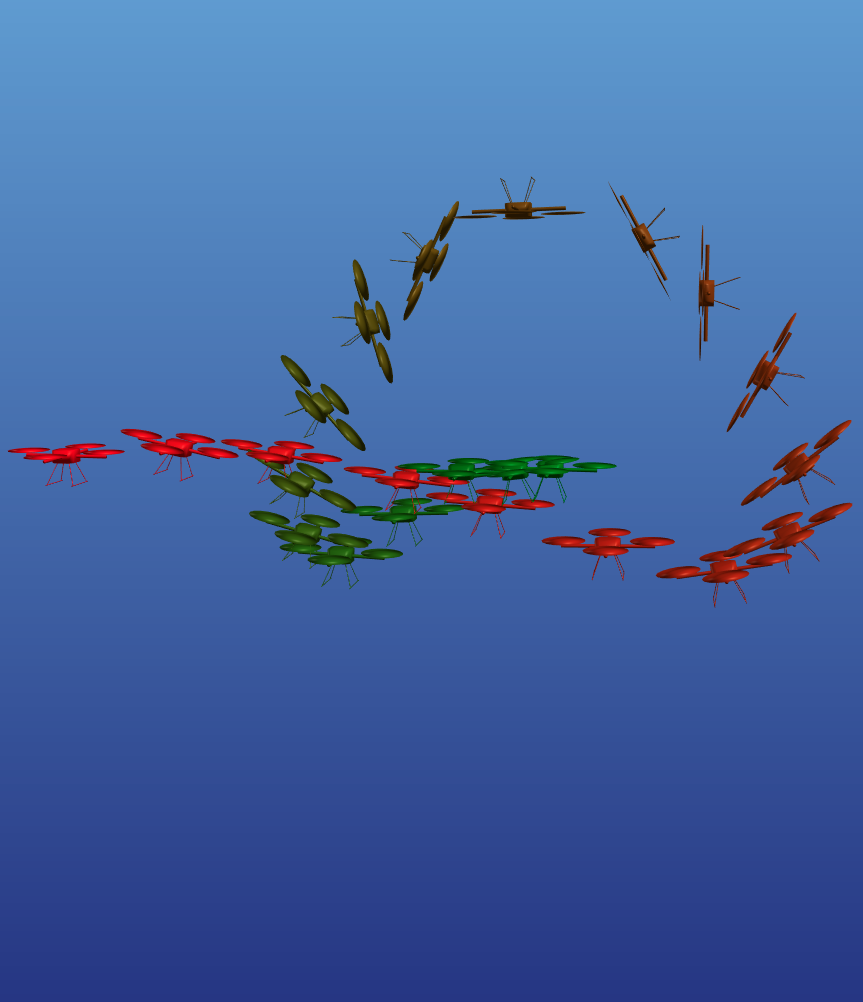
\includegraphics[height=5.2cm,trim={0 3cm 0 0},clip]{figures/quad_flip.png}
                \caption{Snapshots of the quadrotor flip trajectory. The
                    red-colored quadrotors represent the state near t=0 s and the
                    green-colored quadrotors represent the state near t=5.0 s
                }
                \label{fig:quad_flip}
            \end{figure}    

        \subsection{Airplane Barrel Roll}
        An airplane model with aerodynamic coefficients fit from real wind-tunnel data is
        tasked to do a barrel roll by setting a high terminal cost for being upside-down,
        see Fig. \ref{fig:barrellroll}. The solver is initialized with level flight trim
        conditions. For both the quadrotor flip and the airplane barrel roll, iMLQR
        converged faster than the pure quaternion version. Despite the extra matrix
        multiplications and extra Hessian term, it also was faster per iteration than its
        iLQR counterpart. For these highly aerobatic maneuvers, we achieve, as expected,
        better performance by correctly leveraging the structure of the rotation group
        during the optimization routine.
        
        \begin{figure}[h]
            \centering
            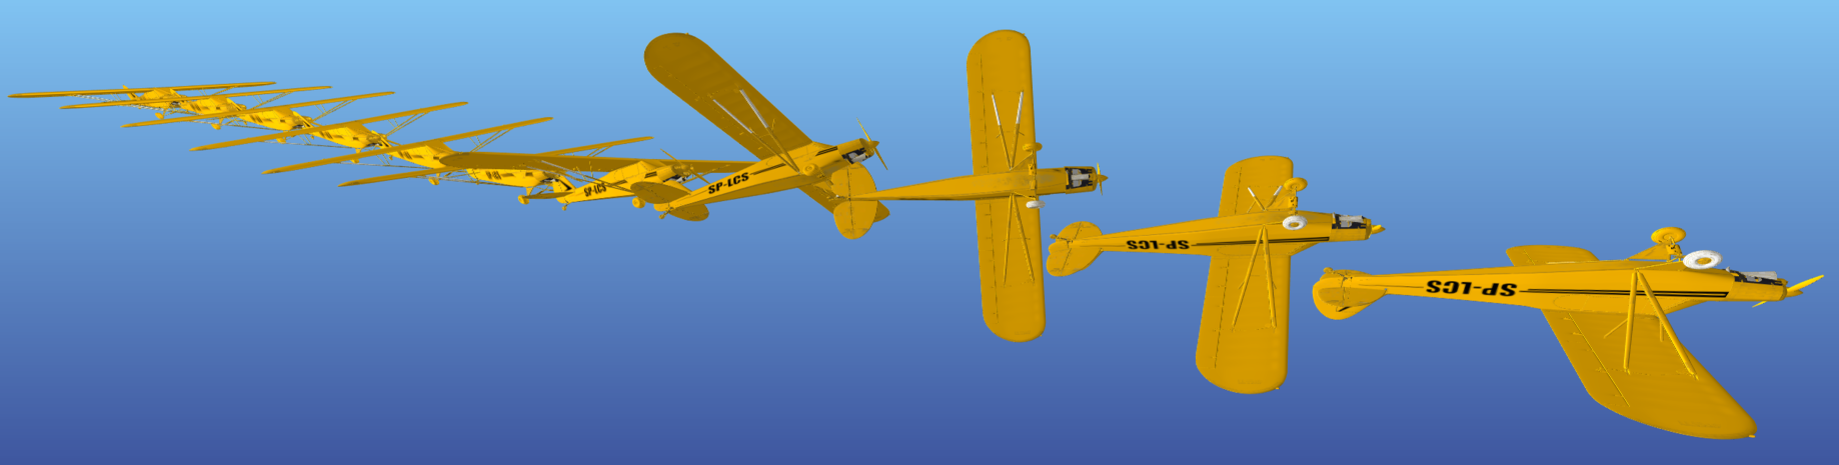
\includegraphics[height=3.5cm]{figures/barrellroll.png}
            \caption{Barrel roll trajectory computed by iterative MLQR using a terminal cost to encourage an upside-down attitude.}
            \label{fig:barrellroll}
        \end{figure}
    

\section{Conclusions} \label{sec:conclusion}
    We have presented a general, unified method for planning and control on rigid-body
    systems with arbitrary attitude using standard linear algebra and vector calculus. By
    applying these methods to LQR to correctly account for the group structure of
    rotations, we have matched or exceeded the performance of a state-of-the-art
    geometric controller designed specifically for quadrotors, while being more general,
    requiring less system-dependent tuning, having less computational overhead, and being
    easier to implement.
    
    We have also demonstrated a straight-forward way to adapt nonlinear trajectory
    optimization techniques to work with quaternion-valued states. For these problems, we
    found the geodesic distance between quaternions \eqref{eq:quat_geodesic} to be
    computationally efficient and provide excellent convergence in practice. We recommend
    the use of unit quaternions within planning and control algorithms for their
    simplicity, computational efficiency, and lack of singularities. We further recommend
    the use of Rodrigues parameters, or the Cayley map, as the quaternion error state.
    
    Future areas of research include the application of these methodologies to more
    complex multi-body floating-base robots, such as humanoids and quadrupeds, as well as
    more in-depth analysis of the convergence behavior of the algorithms proposed in the
    current work.
    
\paragraph{Acknowledgements}
This material is based upon work supported by the National Science Foundation Graduate
Research Fellowship Program under Grant No. DGE-1656518. Any opinions, findings, and
conclusions or recommendations expressed in this material are those of the author(s) and
do not necessarily reflect the views of the National Science Foundation


\printbibliography

\end{document}